% ============================================================
% main.tex - Graduation Project Report
% University of Science and Technology
% Faculty of Engineering - Biomedical Engineering Department
% ============================================================
% Engine: XeLaTeX | Bibliography: biblatex + biber
% ============================================================

\documentclass[12pt, a4paper, oneside]{report}

% ============================================================
% PACKAGES
% ============================================================

% --- Encoding & Fonts ---
\usepackage{fontspec}
\setmainfont{times.ttf}[BoldFont=timesbd.ttf, ItalicFont=timesi.ttf, BoldItalicFont=timesbi.ttf]
\newfontfamily\arabicfont[Script=Arabic, Scale=1.15, BoldFont=artrbdo.ttf, ItalicFont=artro.ttf, ItalicFeatures={AutoFakeSlant=0.18}, BoldItalicFont=artrbdo.ttf, BoldItalicFeatures={AutoFakeSlant=0.18}]{artro.ttf}

% --- Language Support ---
\usepackage{polyglossia}
\setdefaultlanguage{english}
\setotherlanguage[numerals=mashriq]{arabic}

% --- Page Layout (University Requirements) ---
% Binding side: 3.5cm, Other margins: 2.5cm
\usepackage[
  a4paper,
  left=3.5cm,
  right=2.5cm,
  top=2.5cm,
  bottom=2.5cm
]{geometry}

% --- Paragraph & Spacing ---
\usepackage{setspace}
\onehalfspacing
\setlength{\parindent}{1.25cm}
\setlength{\parskip}{0pt}

% --- Headers & Footers ---
\usepackage{fancyhdr}
\pagestyle{fancy}
\fancyhf{}
\fancyhead[R]{\leftmark}
\fancyfoot[C]{\thepage}
\renewcommand{\headrulewidth}{0.4pt}
\renewcommand{\footrulewidth}{0pt}

% Plain style for chapter pages
\fancypagestyle{plain}{
  \fancyhf{}
  \fancyfoot[C]{\thepage}
  \renewcommand{\headrulewidth}{0pt}
}

% --- Colors & Boxes ---
\usepackage[dvipsnames]{xcolor}
\usepackage{tcolorbox}
\definecolor{navyblue}{RGB}{0,51,102}
\definecolor{darkgreen}{RGB}{0,102,51}
\definecolor{darkred}{RGB}{153,0,0}

% --- Section Formatting ---
\usepackage{titlesec}

\usepackage{etoolbox}

% Numbered Chapter Page: Standalone Centered Cover Page
\titleformat{name=\chapter}[display]
  {\thispagestyle{plain}\normalfont\centering\vspace*{4.2cm}}
  {{\color{navyblue}\rule{0.65\textwidth}{1.5pt}}\\[1.5ex]
   \fontsize{18}{22}\selectfont\bfseries\color{navyblue}\MakeUppercase{\chaptertitlename}\ \thechapter}
  {1.2ex}
  {\fontsize{22}{28}\selectfont\bfseries\color{navyblue}\MakeUppercase}
  [\vspace{1.5ex}{\color{navyblue}\rule{0.65\textwidth}{1.5pt}}]

\titlespacing*{name=\chapter}{0pt}{0pt}{0pt}

% Command for elegant chapter overview on the standalone cover page
\newcommand{\chapteroverview}[1]{%
  \vspace{2.0em}%
  \begin{center}%
    \begin{minipage}{0.85\textwidth}%
      \centering\itshape\color{black}%
      \fontsize{11}{16}\selectfont%
      #1%
    \end{minipage}%
  \end{center}%
  \clearpage%
}




% Numberless Chapter Page (TOC, List of Figures/Tables, Abbreviations, References)
\titleformat{name=\chapter,numberless}[display]
  {\normalfont\fontsize{16}{20}\selectfont\bfseries\centering}
  {}{0pt}
  {\fontsize{16}{20}\selectfont\bfseries\MakeUppercase}

\titlespacing*{name=\chapter,numberless}{0pt}{-10pt}{20pt}

% Section title: size 16, bold
\titleformat{\section}
  {\normalfont\fontsize{16}{20}\selectfont\bfseries}
  {\thesection}{1em}{}
\titlespacing*{\section}{0pt}{14pt}{6pt}

% Subsection title: size 12, bold
\titleformat{\subsection}
  {\normalfont\fontsize{12}{16}\selectfont\bfseries}
  {\thesubsection}{1em}{}
\titlespacing*{\subsection}{0pt}{10pt}{4pt}

% Subsubsection title: size 12, bold
\titleformat{\subsubsection}
  {\normalfont\fontsize{12}{16}\selectfont\bfseries}
  {\thesubsubsection}{1em}{}
\titlespacing*{\subsubsection}{0pt}{8pt}{4pt}


% --- Table of Contents, List of Figures/Tables ---
\usepackage{tocloft}
\renewcommand{\cftchapleader}{\cftdotfill{\cftdotsep}}
\renewcommand{\cfttoctitlefont}{\hfill\fontsize{14}{18}\bfseries}
\renewcommand{\cftaftertoctitle}{\hfill}
\renewcommand{\cftloftitlefont}{\hfill\fontsize{14}{18}\bfseries}
\renewcommand{\cftafterloftitle}{\hfill}
\renewcommand{\cftlottitlefont}{\hfill\fontsize{14}{18}\bfseries}
\renewcommand{\cftafterlottitle}{\hfill}
\renewcommand{\cftchappresnum}{Chapter }
\setlength{\cftchapnumwidth}{6.5em}


% --- Graphics ---
\usepackage{graphicx}
\graphicspath{
  {03_Figures/}
  {03_Figures/Ch1/}
  {03_Figures/Ch2/}
  {03_Figures/Ch3/}
  {03_Figures/Ch4/}
  {03_Figures/Ch5/}
  
}

% --- Tables ---
\usepackage{booktabs}
\usepackage{array}
\usepackage{multirow}
\usepackage{longtable}
\usepackage{tabularx}

% --- Captions ---
\usepackage[font={singlespacing,small}, labelfont=bf, labelsep=colon]{caption}
% Table caption on top, figure caption on bottom (university requirement)
\captionsetup[table]{position=above}
\captionsetup[figure]{position=below}

% --- Mathematics ---
\usepackage{amsmath}
\usepackage{amssymb}
\usepackage{amsfonts}
\providecommand{\UseMathForPositioningText}{}

% --- Units ---
\usepackage{siunitx}

% --- TikZ Diagrams ---
\usepackage{tikz}
\usetikzlibrary{shapes.geometric, arrows.meta, positioning, calc, shadows}

% --- Code Listings ---
\usepackage{listings}
\lstset{
  basicstyle=\small\ttfamily,
  breaklines=true,
  frame=single,
  numbers=left,
  numberstyle=\tiny,
  tabsize=4,
  captionpos=b
}

% --- Cross References & Hyperlinks ---
\usepackage[
  colorlinks=true,
  linkcolor=black,
  citecolor=black,
  urlcolor=blue,
  bookmarks=true,
  bookmarksopen=true,
  pdfstartview=FitH
]{hyperref}
\usepackage{bookmark}

% --- Bibliography (IEEE / Numeric Style) ---
\usepackage[
  backend=biber,
  style=numeric,
  sorting=none,
  natbib=true,
  maxcitenames=2,
  maxbibnames=99
]{biblatex}
\addbibresource{references.bib}
% Single-spacing within reference entries and double-spacing between entries
\setlength{\bibitemsep}{2\baselineskip}
\renewcommand{\bibfont}{\normalfont\fontsize{12}{14}\selectfont}



% --- Appendices ---
\usepackage[toc, page]{appendix}

% --- Abbreviations ---
% (Using manual longtable in 07_Abbreviations.tex instead of glossaries package)

% --- List Formatting (University & Academic Standards) ---
\usepackage{enumitem}
\setlist[itemize,1]{label=\textbullet, leftmargin=1.5em, itemsep=3pt, parsep=0pt, topsep=4pt}
\setlist[itemize,2]{label=\textendash, leftmargin=1.5em, itemsep=2pt, parsep=0pt, topsep=2pt}
\setlist[itemize,3]{label=\textcirc, leftmargin=1.5em, itemsep=2pt, parsep=0pt, topsep=2pt}
\setlist[enumerate,1]{label=\textbf{\arabic*.}, leftmargin=1.5em, itemsep=3pt, parsep=0pt, topsep=4pt}
\setlist[enumerate,2]{label=\textbf{(\alph*)}, leftmargin=1.5em, itemsep=2pt, parsep=0pt, topsep=2pt}

% --- Orphan and Widow Control ---
\clubpenalty=10000
\widowpenalty=10000
\displaywidowpenalty=10000

\usepackage{float}
\usepackage{placeins}
\usepackage{subcaption}
\usepackage{pdfpages}

% --- Float Placement Parameters ---
\renewcommand{\topfraction}{0.85}
\renewcommand{\bottomfraction}{0.85}
\renewcommand{\textfraction}{0.15}
\renewcommand{\floatpagefraction}{0.75}


% ============================================================
% CUSTOM COMMANDS
% ============================================================

% Arabic text inline
\newcommand{\ar}[1]{\textarabic{#1}}

% ============================================================
% DOCUMENT METADATA
% ============================================================

\hypersetup{
  pdftitle={Graduation Project Report},
  pdfauthor={Student Name},
  pdfsubject={Biomedical Engineering Graduation Project},
  pdfkeywords={EOG, Wheelchair, Arabic Keyboard, Biomedical Engineering}
}

% ============================================================
% DOCUMENT BEGIN
% ============================================================
\begin{document}

% --- Front Matter (Roman numerals) ---
\pagenumbering{roman}
\pagestyle{plain}

% Title Page
% ============================================================
% Title Page (Official UST Past-Year Matching Standard)
% ============================================================
\begin{titlepage}
\centering

\vspace*{-0.4cm}

% --- Header Information ---
{\fontsize{13}{16}\selectfont\bfseries Republic of Yemen}\\[0.12cm]
{\fontsize{14}{17}\selectfont\bfseries University of Science and Technology}\\[0.12cm]
{\fontsize{13}{16}\selectfont\bfseries Faculty of Engineering and Computing}\\[0.1cm]
{\fontsize{12}{15}\selectfont\bfseries Department of Biomedical Engineering}\\[0.35cm]

% --- Official University Logo ---

\includegraphics[height=2.6cm]{ust_logo.png}\\[0.35cm]

% --- Upper Divider Rule ---
\rule{0.92\textwidth}{1.2pt}\\[0.45cm]

% --- Project Title (Crisp, Proportional Size) ---
{\fontsize{15}{21}\selectfont\bfseries Design and Implementation of an Integrated\\
EOG-Based Human-Computer Interface for\\
Virtual Keyboard and Wheelchair Control}\\[0.45cm]

% --- Lower Divider Rule ---
\rule{0.92\textwidth}{1.2pt}\\[0.5cm]

% --- Research Prepared by Section ---
{\fontsize{12}{15}\selectfont\bfseries Research prepared by:}\\[0.25cm]
{\fontsize{11}{16}\selectfont
1. Abdulaziz Khaled Abdulaziz Hatem\\[0.08cm]
2. Ahmed Mohammed Ahmed Salem Al-Kadhi\\[0.08cm]
3. Mohammed Ayman Ali Qasem\\[0.08cm]
4. Khaled Abdulmajid Mohammed Farhan}\\[0.5cm]

% --- Supervised by Section ---
{\fontsize{12}{15}\selectfont\bfseries Supervised by:}\\[0.2cm]
{\fontsize{11}{15}\selectfont Dr. Nasr Kaid Ali AL-Audi}\\[0.6cm]

% --- Degree Statement (Exact Official Wording) ---
{\fontsize{10.5}{14}\selectfont\itshape (To the Faculty of Engineering and Computing, This Research is a Part of the\\
Requirements for Obtaining a Bachelor's Degree in Biomedical Engineering)}\\[0.4cm]

\vfill

% --- Academic Year ---
{\fontsize{11}{14}\selectfont\bfseries 2025 - 2026}

\end{titlepage}


% Dedication
% ============================================================
% Dedication (الإهداء) - Guaranteed Slanted/Italic Arabic
% ============================================================
\thispagestyle{empty}
\vspace*{\fill}

\begin{center}
\begin{Arabic}
{\fontsize{20}{24}\selectfont\bfseries\itshape الإهداء}
\end{Arabic}
\end{center}
\vspace{1.2cm}

\begin{center}
\begin{Arabic}
\fontsize{13}{24}\selectfont
\setstretch{1.65}
\itshape

الحمد لله الذي وهبنا الإرادة، وذلل لنا سبل العلم، وأعاننا بفضله حتى بلغنا تمام هذا العمل..\\[1.2em]

{\bfseries\itshape نهدي ثمرة جهدنا وسهرنا:}\\[1.2em]

إلى من كانت دعواتهم طوق نجاةٍ لنا في لحظات التعب، وإلى العيون التي سهرت تترقب نجاحنا.. آبائنا وأمهاتنا؛ كنزنا الأغلى، والسند الذي لا يميل.\\[1.2em]

إلى القلوب التي استلهمنا من صمتها الفكرة، ومن صلابة إرادتها العزيمة.. أصحاب الهمم من مرضى التصلب الجانبي الضموري، ومتلازمة المنحبس، والشلل الرباعي. نهديكم هذا الجهد بيقين وحب، عسى أن يكون يداً حانية ترد لكم شيئاً من استقلاليتكم، ونافذة أملٍ تكسر حاجز الصمت وتصلكم بالعالم.\\[1.2em]

إلى إخوتنا، دفء الأيام وملاذنا الآمن.. وإلى أصدقاء المسيرة ورفاق الدرب، الذين تقاسمنا معهم ثقل البدايات ولذة النهايات، وكانوا لنا خير سندٍ ورفقة.\\[1.2em]

وإلى كل قلبٍ آمن بنا، وساندنا ولو بكلمة تشجيع صادقة..\\[1.2em]

إليكم جميعاً نهدي هذا العمل المتواضع.

\end{Arabic}
\end{center}

\vspace*{\fill}
\clearpage


% Acknowledgments
% ============================================================
% Acknowledgments (الشكر والعرفان) - Arabic Format
% ============================================================
\thispagestyle{plain}
\vspace*{0.5cm}

\begin{center}
\begin{Arabic}
{\fontsize{18}{22}\selectfont\bfseries الشكر والعرفان}
\end{Arabic}
\end{center}
\vspace{0.6cm}

\begin{Arabic}
\fontsize{12}{22}\selectfont
\setstretch{1.6}

الحمد لله رب العالمين، حمداً يليق بجلال وجهه وعظيم سلطانه، على ما أنعم به علينا من توفيق وهداية، وما وهبنا من قدرة وصبر حتى وصلنا إلى إتمام هذا البحث وتكليل مسيرتنا العلمية بهذا الإنجاز.

وعملاً بالهدي النبوي الشريف: «مَنْ لا يَشْكُرُ النَّاسَ لا يَشْكُرُ اللَّهَ»، يُسعدنا ويشرّفنا أن نتقدم ببالغ الشكر وعظيم الامتنان إلى مشرف مشروعنا الفاضل \textbf{الدكتور نصر قايد علي العودي}، الذي كان لنصائحه القيمة وتوجيهاته الأكاديمية السديدة ومتابعته الدؤوبة أبلغ الأثر في تذليل الصعاب وتوجيه مسار هذا العمل الهندسي نحو أهدافه المرجوة.

كما نتقدم بخالص الشكر والتقدير إلى جميع أساتذتنا الأفاضل في \textbf{قسم الهندسة الحيوية الطبية} و\textbf{كلية الهندسة} في جامعة العلوم والتكنولوجيا، الذين لم يدخروا جهداً في تزويدنا بالعلوم والمعارف وإرساء القواعد العلمية والهندسية المتينة طوال سنوات دراستنا الجامعية.

ونتوجه بالشكر إلى كل من قدم لنا يد العون والمساعدة، أو أسدى إلينا نصيحة تقنية، أو دعمنا بكلمة مشجعة كان لها أثر طيب في إنجاح هذا العمل.

نسأل الله العلي القدير أن يبارك في هذا الجهد، وأن يجعله نافعاً وخالصاً لوجهه الكريم، وأن يجزيهم جميعاً عنا خير الجزاء.

\end{Arabic}

\normalsize
\clearpage


% Abstract
% ============================================================
% Abstract (English & Arabic) - Standard UST Spacing Layout
% ============================================================
\thispagestyle{plain}
\vspace*{0.2cm}

% --- English Abstract Header ---
\begin{center}
{\fontsize{15}{18}\selectfont\bfseries ABSTRACT}
\end{center}
\vspace{0.2cm}

\fontsize{11}{16.5}\selectfont
\setstretch{1.45}
This project presents an integrated assistive platform designed for individuals with severe motor disabilities, such as quadriplegia, locked-in syndrome, ALS, and muscular dystrophy, who retain voluntary eye movement. The platform integrates motorized wheelchair navigation and virtual keyboard communication into a unified assistive system controlled via Electrooculography (EOG) signals. The technical architecture comprises a discrete EOG analog front-end with an AD620 instrumentation amplifier, digital filtering in MATLAB (250~Hz sampling rate, moving-average smoothing, and 50~Hz notch filtering), and an Arduino microcontroller with ultrasonic obstacle detection. Preliminary evaluation across five healthy subjects yielded an overall command execution accuracy of 92\% and a mean text entry rate of 16 characters per minute (CPM), demonstrating the operational feasibility of the low-cost prototype.

\vspace{0.8cm}

% --- Arabic Abstract Header ---
\begin{center}
\begin{Arabic}
{\fontsize{15}{18}\selectfont\bfseries المستخلص}
\end{Arabic}
\end{center}
\vspace{0.2cm}

\begin{Arabic}
\fontsize{11.5}{18}\selectfont
\setstretch{1.65}
يُقدم هذا المشروع تصميماً هندسياً لمنصة مساعدة مدمجة تلبي احتياجات الأفراد الذين يعانون من إعاقات حركية شديدة (مثل الشلل الرباعي، متلازمة الانحباس، التصلب الجانبي الضموري ALS، وضمور العضلات) مع احتفاظهم بحركة العين الإرادية. يدمج النظام وظيفتين أساسيتين؛ وهما التحكم في كرسي متحرك بمحركات كهربائية، والتواصل عبر لوحة مفاتيح افتراضية، داخل نظام موحد يعتمد على إشارات حركة العين (Electrooculography - EOG). تعتمد المعمارية التقنية على دائرة تماثلية مخصصة لاكتساب الإشارة وتكبيرها باستخدام مكبر الأجهزة (AD620)، متبوعة بترشيح رقمي عبر بيئة MATLAB بمعدل أخذ عينات 250~Hz ومرشح إيقاف حزمة 50~Hz. أظهرت الاختبارات المعملية الأولية على خمسة متطوعين أصحاء دقة تنفيذ أوامر بلغت 92\% ومتوسط سرعة كتابة 16 حرفاً في الدقيقة، مدعوماً بنظام أمان لتفادي العوائق عبر حساسات الموجات فوق الصوتية، مما يؤكد الجدوى التشغيلية لهذا النموذج الأولي منخفض التكلفة.
\end{Arabic}

\normalsize
\clearpage


% Table of Contents
\input{00_Frontmatter/05_Table_of_Contents}

% List of Tables
% ============================================================
% List of Tables
% ============================================================
\listoftables
\addcontentsline{toc}{chapter}{List of Tables}
\clearpage


% List of Figures
% ============================================================
% List of Figures
% ============================================================
\listoffigures
\addcontentsline{toc}{chapter}{List of Figures}
\clearpage


% Abbreviations
% ============================================================
% List of Abbreviations
% ============================================================
\chapter*{List of Abbreviations}
\addcontentsline{toc}{chapter}{List of Abbreviations}

\begin{longtable}{@{}p{3cm}p{10cm}@{}}
\toprule
\textbf{Abbreviation} & \textbf{Description} \\
\midrule
\endhead
ADC   & Analog-to-Digital Converter \\
BMS   & Battery Management System \\
CMRR  & Common-Mode Rejection Ratio \\
EEG   & Electroencephalography \\
EMG   & Electromyography \\
EOG   & Electrooculography \\
FSM   & Finite State Machine \\
GUI   & Graphical User Interface \\
HPF   & High-Pass Filter \\
LIS   & Locked-in Syndrome \\
LPF   & Low-Pass Filter \\
MCU   & Microcontroller Unit \\
PCB   & Printed Circuit Board \\
PWM   & Pulse-Width Modulation \\
\bottomrule
\end{longtable}


% --- Main Matter (Arabic numerals) ---
\pagenumbering{arabic}
\pagestyle{fancy}

% Chapter 1: Introduction
% ============================================================
% Chapter 1: Introduction
% ============================================================
\chapter{Introduction}
\label{ch:introduction}

\chapteroverview{This chapter introduces the fundamental clinical background, problem statement, and engineering objectives of the proposed EOG-based assistive technology system. It contextualizes non-invasive Human-Machine Interfaces (HMIs) for patients with Locked-in Syndrome (LIS), outlines the specific project goals, presents the structure of the thesis report, and details the two-year engineering milestone execution timeline.}


% ============================================================
% Section 1.1: General Overview and Clinical Background
% ============================================================
\section{General Overview and Clinical Background}
\label{sec:general_overview_clinical_background}

Severe neurodegenerative disorders and traumatic injuries---such as advanced Amyotrophic Lateral Sclerosis (ALS), Muscular Dystrophy, brainstem stroke, and high-level spinal cord injuries---frequently result in profound motor paralysis, often presenting as Locked-in Syndrome (LIS) or Quadriplegia. Patients in these clinical conditions suffer from a complete loss of voluntary muscle control throughout the body, depriving them of conventional speech and physical interaction with their environment. However, the cranial nerves controlling extraocular muscle motility remain physiologically intact and functionally operational in most affected individuals.

To address these severe functional deficits, non-invasive Human-Machine Interfaces (HMIs) based on electrooculography (EOG) have emerged as an effective assistive solution. EOG exploits the standing electrostatic potential maintained between the cornea and the retina to track eye displacement and voluntary eyelid blinks.


% ============================================================
% Section 1.2: Problem Statement
% ============================================================
\section{Problem Statement}
\label{sec:problem_statement}

Individuals with severe motor paralysis face extreme social isolation and total reliance on caregivers due to the lack of functional communication and mobility tools. Although various assistive technologies currently exist, they present major technical and practical limitations. First, invasive Brain-Computer Interfaces (BCIs) provide direct neural control but carry significant surgical risks, tissue infection hazards, and high financial costs. Second, Video-Oculography (VOG) camera-based eye-tracking alternatives are highly sensitive to ambient lighting variations, require continuous spatial calibration, and demand high computational processing power. Third, system fragmentation remains a major barrier, as most commercially available devices treat communication and physical locomotion as separate challenges, requiring independent and expensive standalone platforms for each function.


Consequently, an engineering need exists for a non-invasive, low-cost HMI with reliable threshold detection. Such a system must utilize simplified biopotential acquisition hardware to deliver real-time control over both digital text communication and motorized mobility platforms within a single interface.

This project presents the design and implementation of an assistive technology system that integrates a virtual keyboard for text-based communication and a prototype motorized wheelchair controlled via real-time EOG thresholding. This framework addresses mobility and communication requirements within a single, unified platform.


% ============================================================
% Section 1.3: Project Engineering Objectives
% ============================================================
\section{Project Engineering Objectives}
\label{sec:project_engineering_objectives}

The primary objective of this project is to develop an integrated, cost-effective, non-invasive HMI that provides individuals with locked-in syndrome (LIS) an assistive interface for communication and navigation. To attain this overall goal, the following specific engineering objectives were established:

\begin{enumerate}[label=\textbf{\arabic*.}]
    \item \textbf{Bio-Potential Acquisition Hardware Design:} To design and assemble a high-gain, low-noise analog front-end circuit capable of reliably capturing microvolt-level corneo-retinal potentials while rejecting power-line interference and environmental electromagnetic noise.
    \item \textbf{Real-Time Signal Processing Framework:} To implement real-time digital filtering and thresholding algorithms within a hybrid MATLAB-Arduino processing architecture to extract and classify the temporal characteristics of voluntary eye blinks.
    \item \textbf{Finite State Machine Control Integration:} To engineer a deterministic Finite State Machine (FSM) that translates multi-blink sequences into operational commands, allowing a single biopotential channel to manage two distinct subsystems while enforcing safety protocols.
    \item \textbf{Virtual Optical Speller Development:} To construct an auto-scanning virtual keyboard featuring a Graphical User Interface (GUI) configured to reduce cognitive load, enabling users to compose, edit, and clear text.
    \item \textbf{3D-Printed Prototype Wheelchair Implementation:} To construct a functional 3D-printed motorized wheelchair prototype that receives wireless directional commands, serving as a scaled experimental model to validate wheelchair navigation and obstacle-avoidance logic.
\end{enumerate}

% ============================================================
% Section 1.4: Report Organization
% ============================================================
\section{Report Organization}
\label{sec:report_organization}

This thesis is organized into six main chapters structured logically to document the complete engineering lifecycle of the EOG-based assistive system:

\begin{itemize}
    \item \textbf{Chapter 1 (Introduction):} Outlines the clinical background, problem statement, engineering objectives, thesis structure, and execution timeline.
    \item \textbf{Chapter 2 (Literature Review and Theoretical Background):} Reviews existing literature on biopotential acquisition, HMIs, virtual spellers, and eye-tracking systems while identifying current technical gaps.
    \item \textbf{Chapter 3 (System Architecture and Block Diagram):} Details the high-level architecture, functional block diagrams, operational mode-switching logic, and overall system flowcharts.
    \item \textbf{Chapter 4 (Circuit Simulation and Hardware Implementation):} Presents circuit simulations, mathematical design calculations, component selection (AD620, L298N), and software architecture.
    \item \textbf{Chapter 5 (Results and Discussion):} Evaluates experimental biopotential waveforms, obstacle avoidance response times, virtual speller accuracy, and statistical performance metrics.
    \item \textbf{Chapter 6 (Conclusion and Recommendations):} Synthesizes the core engineering findings, clinical applications, and provides strategic recommendations for future technical developments.
\end{itemize}

% ============================================================
% Section 1.5: Project Execution Timeline
% ============================================================
\section{Project Execution Timeline}
\label{sec:project_execution_timeline}

The development lifecycle of this project was systematically organized across two academic years (within the four-year Biomedical Engineering curriculum).

During Year 3, efforts focused on EOG signal acquisition, continuous hardware design, noise suppression, and circuit optimization until a stable signal output was achieved. Building upon this hardware foundation, Year 4 focused on software development, virtual keyboard GUI programming, finite state machine integration, 3D printing of the prototype vehicle, and wireless control integration. Table \ref{tab:project_timeline} summarizes the engineering milestones achieved across this timeline.

\begin{table}[H]
  \centering
  \caption{Two-Year Project Execution Timeline (Year 3 -- Year 4)}
  \label{tab:project_timeline}
  \begin{tabularx}{\textwidth}{l X c}
    \toprule
    \textbf{Stage} & \textbf{Engineering Task \& Technical Focus} & \textbf{Academic Period} \\
    \midrule
    Phase 1 & Clinical background research, initial EOG signal acquisition, and preliminary analog circuit prototyping & Year 3 -- Semester 1 \\
    Phase 2 & Hardware optimization, active filter tuning, and achieving stable signal acquisition & Year 3 -- Semester 2 \\
    Phase 3 & Virtual keyboard programming (GUI), FSM control logic implementation, and signal algorithm refinement & Year 4 -- Semester 1 \\
    Phase 4 & 3D-printed vehicle construction, wireless control integration, system validation testing, and final documentation & Year 4 -- Semester 2 \\
    \bottomrule
  \end{tabularx}
\end{table}


% --- Chapter Conclusion & Transition ---
\vspace{1em}
In summary, this introductory chapter established the clinical motivation, engineering scope, and milestone timeline of the proposed EOG-guided assistive system. Having outlined the foundational objectives for vehicle mobility and virtual speller communication, Chapter 2 reviews relevant literature, the electrophysiology of the corneo-retinal dipole, and biopotential conditioning principles.


% Chapter 2: Medical & Engineering Background and Literature Review
% ============================================================
% Chapter 2: Literature Review and Theoretical Background
% ============================================================
\chapter{Literature Review and Theoretical Background}
\label{ch:background}

\chapteroverview{This chapter provides the theoretical and scientific foundation supporting the proposed integrated assistive system. It begins with the medical background necessary to understand the biophysical nature and origin of electrooculography (EOG) signals. It then discusses the fundamental engineering principles related to biomedical signal acquisition, digital signal processing, and physical control systems. Furthermore, the chapter presents a literature review of previous studies in the field of eye-tracking and biomedical assistive technologies. Finally, it concludes by highlighting the advantages of the adopted technical approach and demonstrating the technical feasibility of this integrated design.}


% ============================================================
% Section 2.1: Medical Background
% ============================================================
\section{Medical Background}
\label{sec:medical_background}

\subsection{Anatomy and Physiology of the Human Eye (Corneo-Retinal Dipole)}
\label{subsec:anatomy_eye_dipole}

From an electrical perspective, the human eye functions as a biological dipole or bio-battery. This electrostatic property arises from the resting potential difference maintained between the cornea and the retina. The anterior segment (cornea) carries a positive electrical charge, whereas the posterior segment (retina) carries a negative charge. This charge distribution generates an internal standing potential ranging from $10\,\text{mV}$ to $30\,\text{mV}$ \cite{webster2009medical}. However, when measured at the skin surface, this potential experiences significant attenuation due to the impedance of surrounding biological tissues. As the eyeball rotates, the orientation and magnitude of this electrostatic field shift relative to fixed electrode placement sites on the face. Figure \ref{fig:corneo_retinal_dipole} illustrates this corneo-retinal dipole mechanism and the resulting voltage variation observed at the skin surface during horizontal eye movements.

\begin{figure}[H]
  \centering
  \includegraphics[width=0.75\textwidth]{Graphical-illustration-of-the-corneo-retinal-standing-potential-of-the-eyeball.png}
  \caption{Corneo-retinal dipole potential and signal variations during eye movements \cite{dietrich2017towards}.}
  \label{fig:corneo_retinal_dipole}
\end{figure}

\FloatBarrier
\subsection{Biomechanics of Eye Movements and Blinks}
\label{subsec:biomechanics_eye_movements}

Human ocular dynamics consist primarily of rapid ballistic movements known as saccades and stationary resting intervals referred to as fixations. In addition, eyelid activity (blinking) can be physiologically categorized into involuntary and voluntary blinks. Involuntary blinks occur spontaneously to lubricate the corneal surface, whereas voluntary blinks are intentional, displaying significantly higher signal amplitudes and longer durations \cite{hall2016guyton}. Distinguishing between these two physiological behaviors is essential for the system's control logic. The software algorithm relies on detecting intentional, strong blinks and sustained fixations to generate mode-switching and selection commands while filtering out random involuntary blinks to prevent false system activation.

To distinguish between spontaneous eyelid activity and intentional control commands, the temporal and amplitude characteristics of the biopotential waveforms were analyzed. As illustrated in Figure \ref{fig:eog_blink_thresholding}(A), an involuntary blink produces a narrow, lower-amplitude biphasic spike with a short temporal footprint ($\approx 150\,\text{ms}$) resulting from spontaneous corneal lubrication. Conversely, as depicted in Figure \ref{fig:eog_blink_thresholding}(B), an intentional voluntary blink yields a significantly wider peak with a higher voltage amplitude and an extended temporal duration ($>400\,\text{ms}$) caused by conscious eyelid muscle contraction. These amplitude and temporal width disparities form the physiological basis for real-time command classification.

\begin{figure}[H]
  \centering
  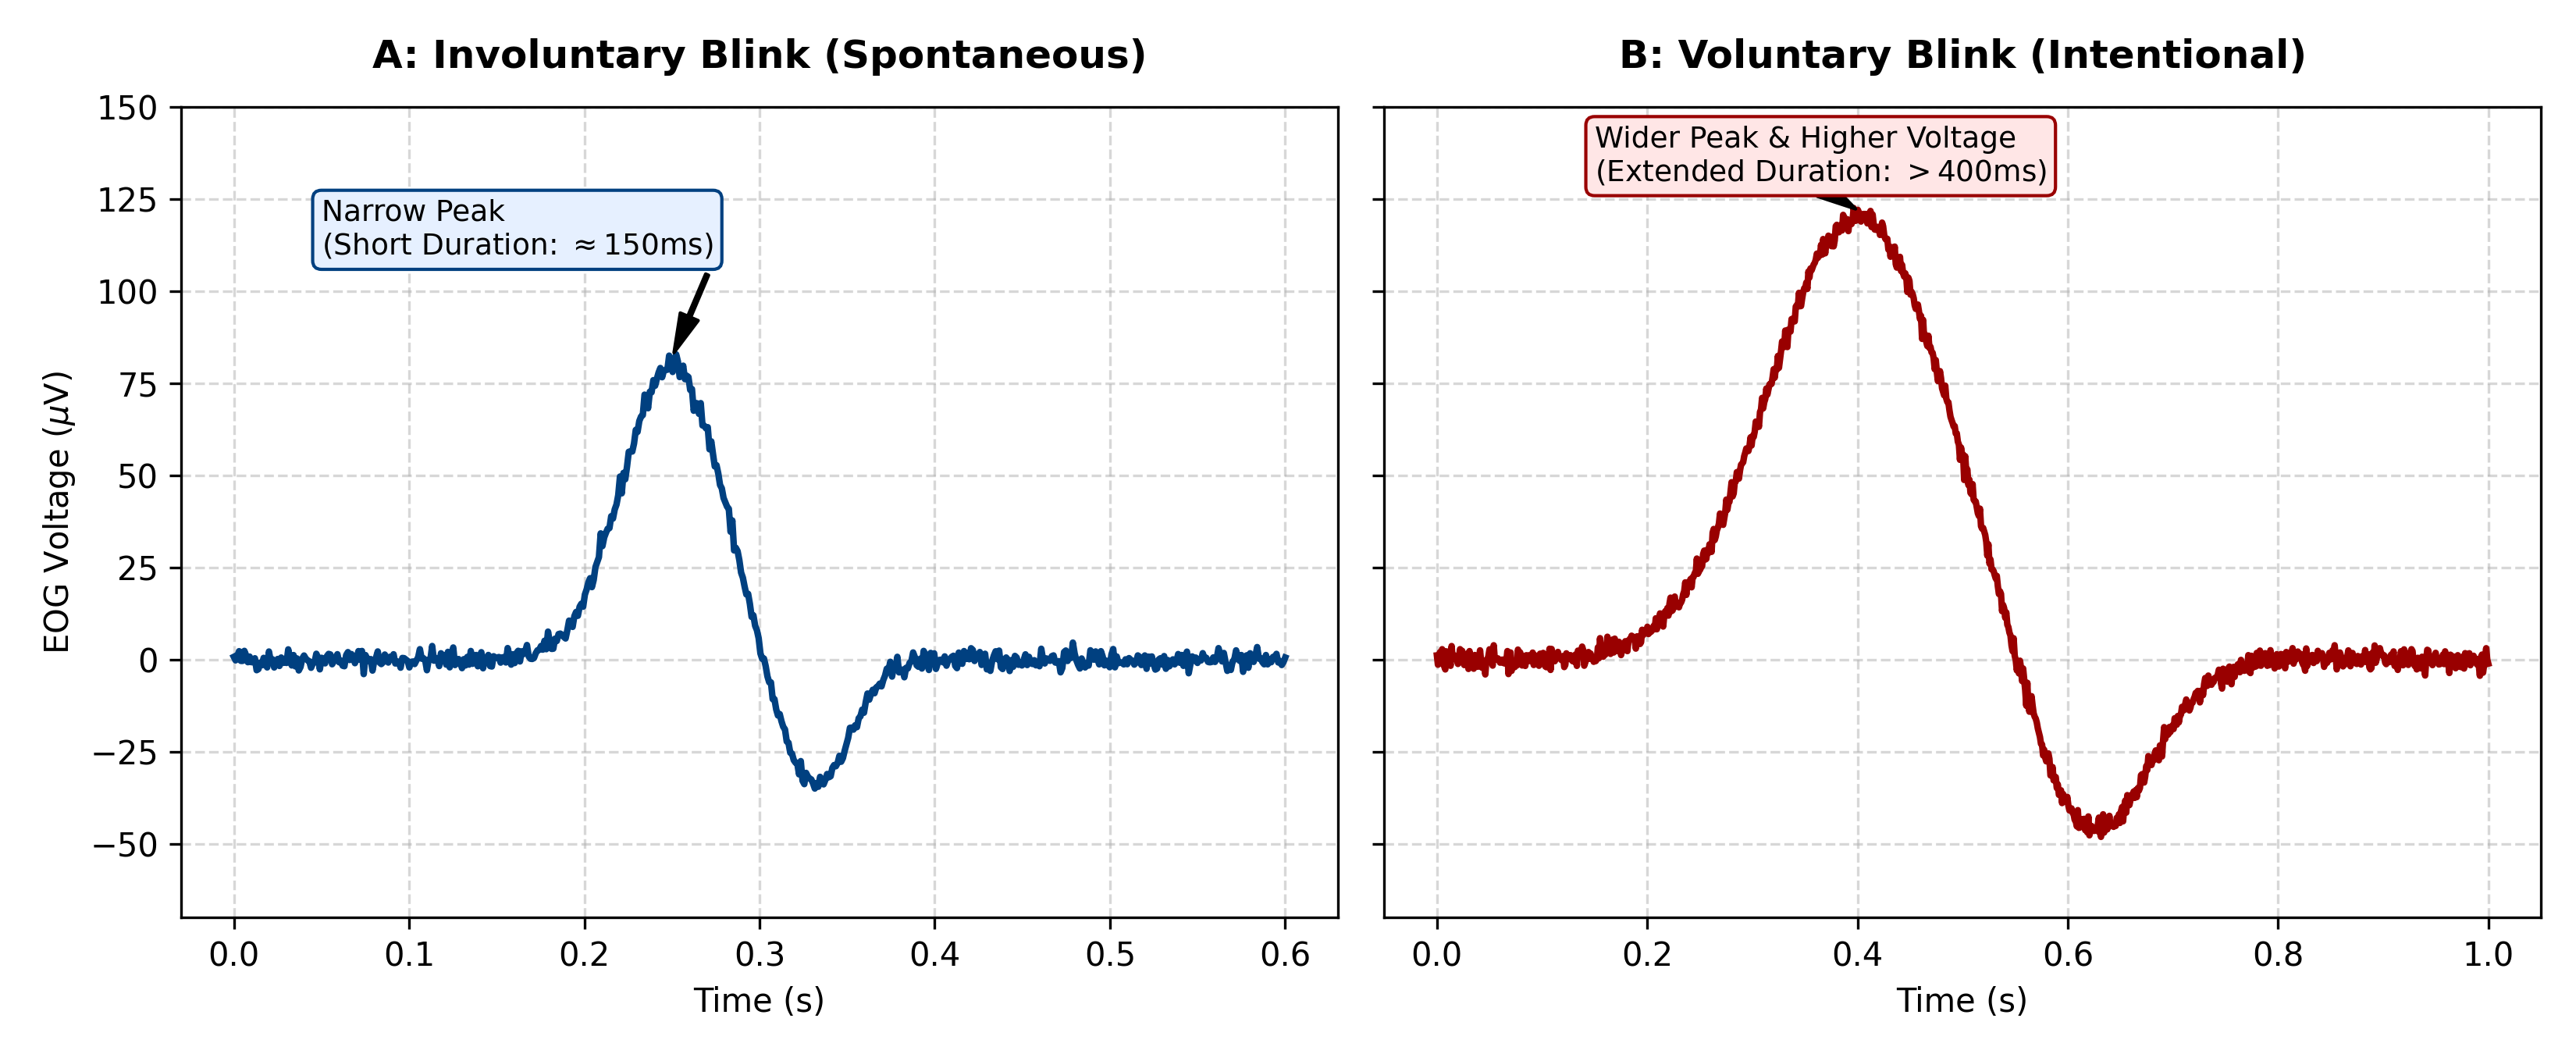
\includegraphics[width=0.95\textwidth]{eog_blink_thresholding.png}
  \caption{Comparison of EOG signal waveforms: (A) Spontaneous involuntary blink displaying a narrow peak and short duration ($\approx 150\,\text{ms}$); (B) Intentional voluntary blink exhibiting a wider peak, higher voltage amplitude, and extended duration ($>400\,\text{ms}$).}
  \label{fig:eog_blink_thresholding}
\end{figure}

\FloatBarrier
\subsection{Characteristics of the Electrooculography (EOG) Signal}
\label{subsec:eog_characteristics_detail}

The electrooculography (EOG) signal possesses specific biophysical characteristics that dictate the design requirements of the signal conditioning hardware. The amplitude of raw surface-measured EOG signals typically ranges from $10\,\mu\text{V}$ to $5\,\text{mV}$, necessitating high-precision differential instrumentation amplifiers. In terms of frequency distribution, the fundamental power spectrum of interest for ocular movement spans from $0.1\,\text{Hz}$ to $30\,\text{Hz}$ \cite{webster2009medical}. Based on these biophysical properties, a hardware low-pass filter with a cut-off frequency of $30\,\text{Hz}$ was implemented to eliminate unwanted high-frequency noise. Furthermore, to isolate the DC offset component and shape the signal into sharp, well-defined pulses (spikes) corresponding to voluntary blinks, the cut-off frequency of the high-pass filter was set to $0.8\,\text{Hz}$.

\FloatBarrier
\subsection{Physiological Principles of Electrode Placement}
\label{subsec:electrode_placement}

Acquiring high-quality EOG signals requires proper anatomical positioning of surface electrodes. To capture the vertical channel (corresponding to vertical eye movements and eyelid blinks), electrodes are attached directly above and below one eye. For the horizontal channel, electrodes are placed at the lateral margins of both eyes, near the outer canthi. This configuration measures differential potential changes as the corneo-retinal dipole rotates toward or away from a given electrode, while a reference electrode positioned on the forehead provides a ground potential to cancel common-mode interference \cite{webster2009medical}. To illustrate the vertical channel electrode configuration described above, Figure \ref{fig:vertical_eog_placement} depicts the anatomical positioning of the supra-orbital and infra-orbital electrodes used in this project.

\begin{figure}[H]
  \centering
  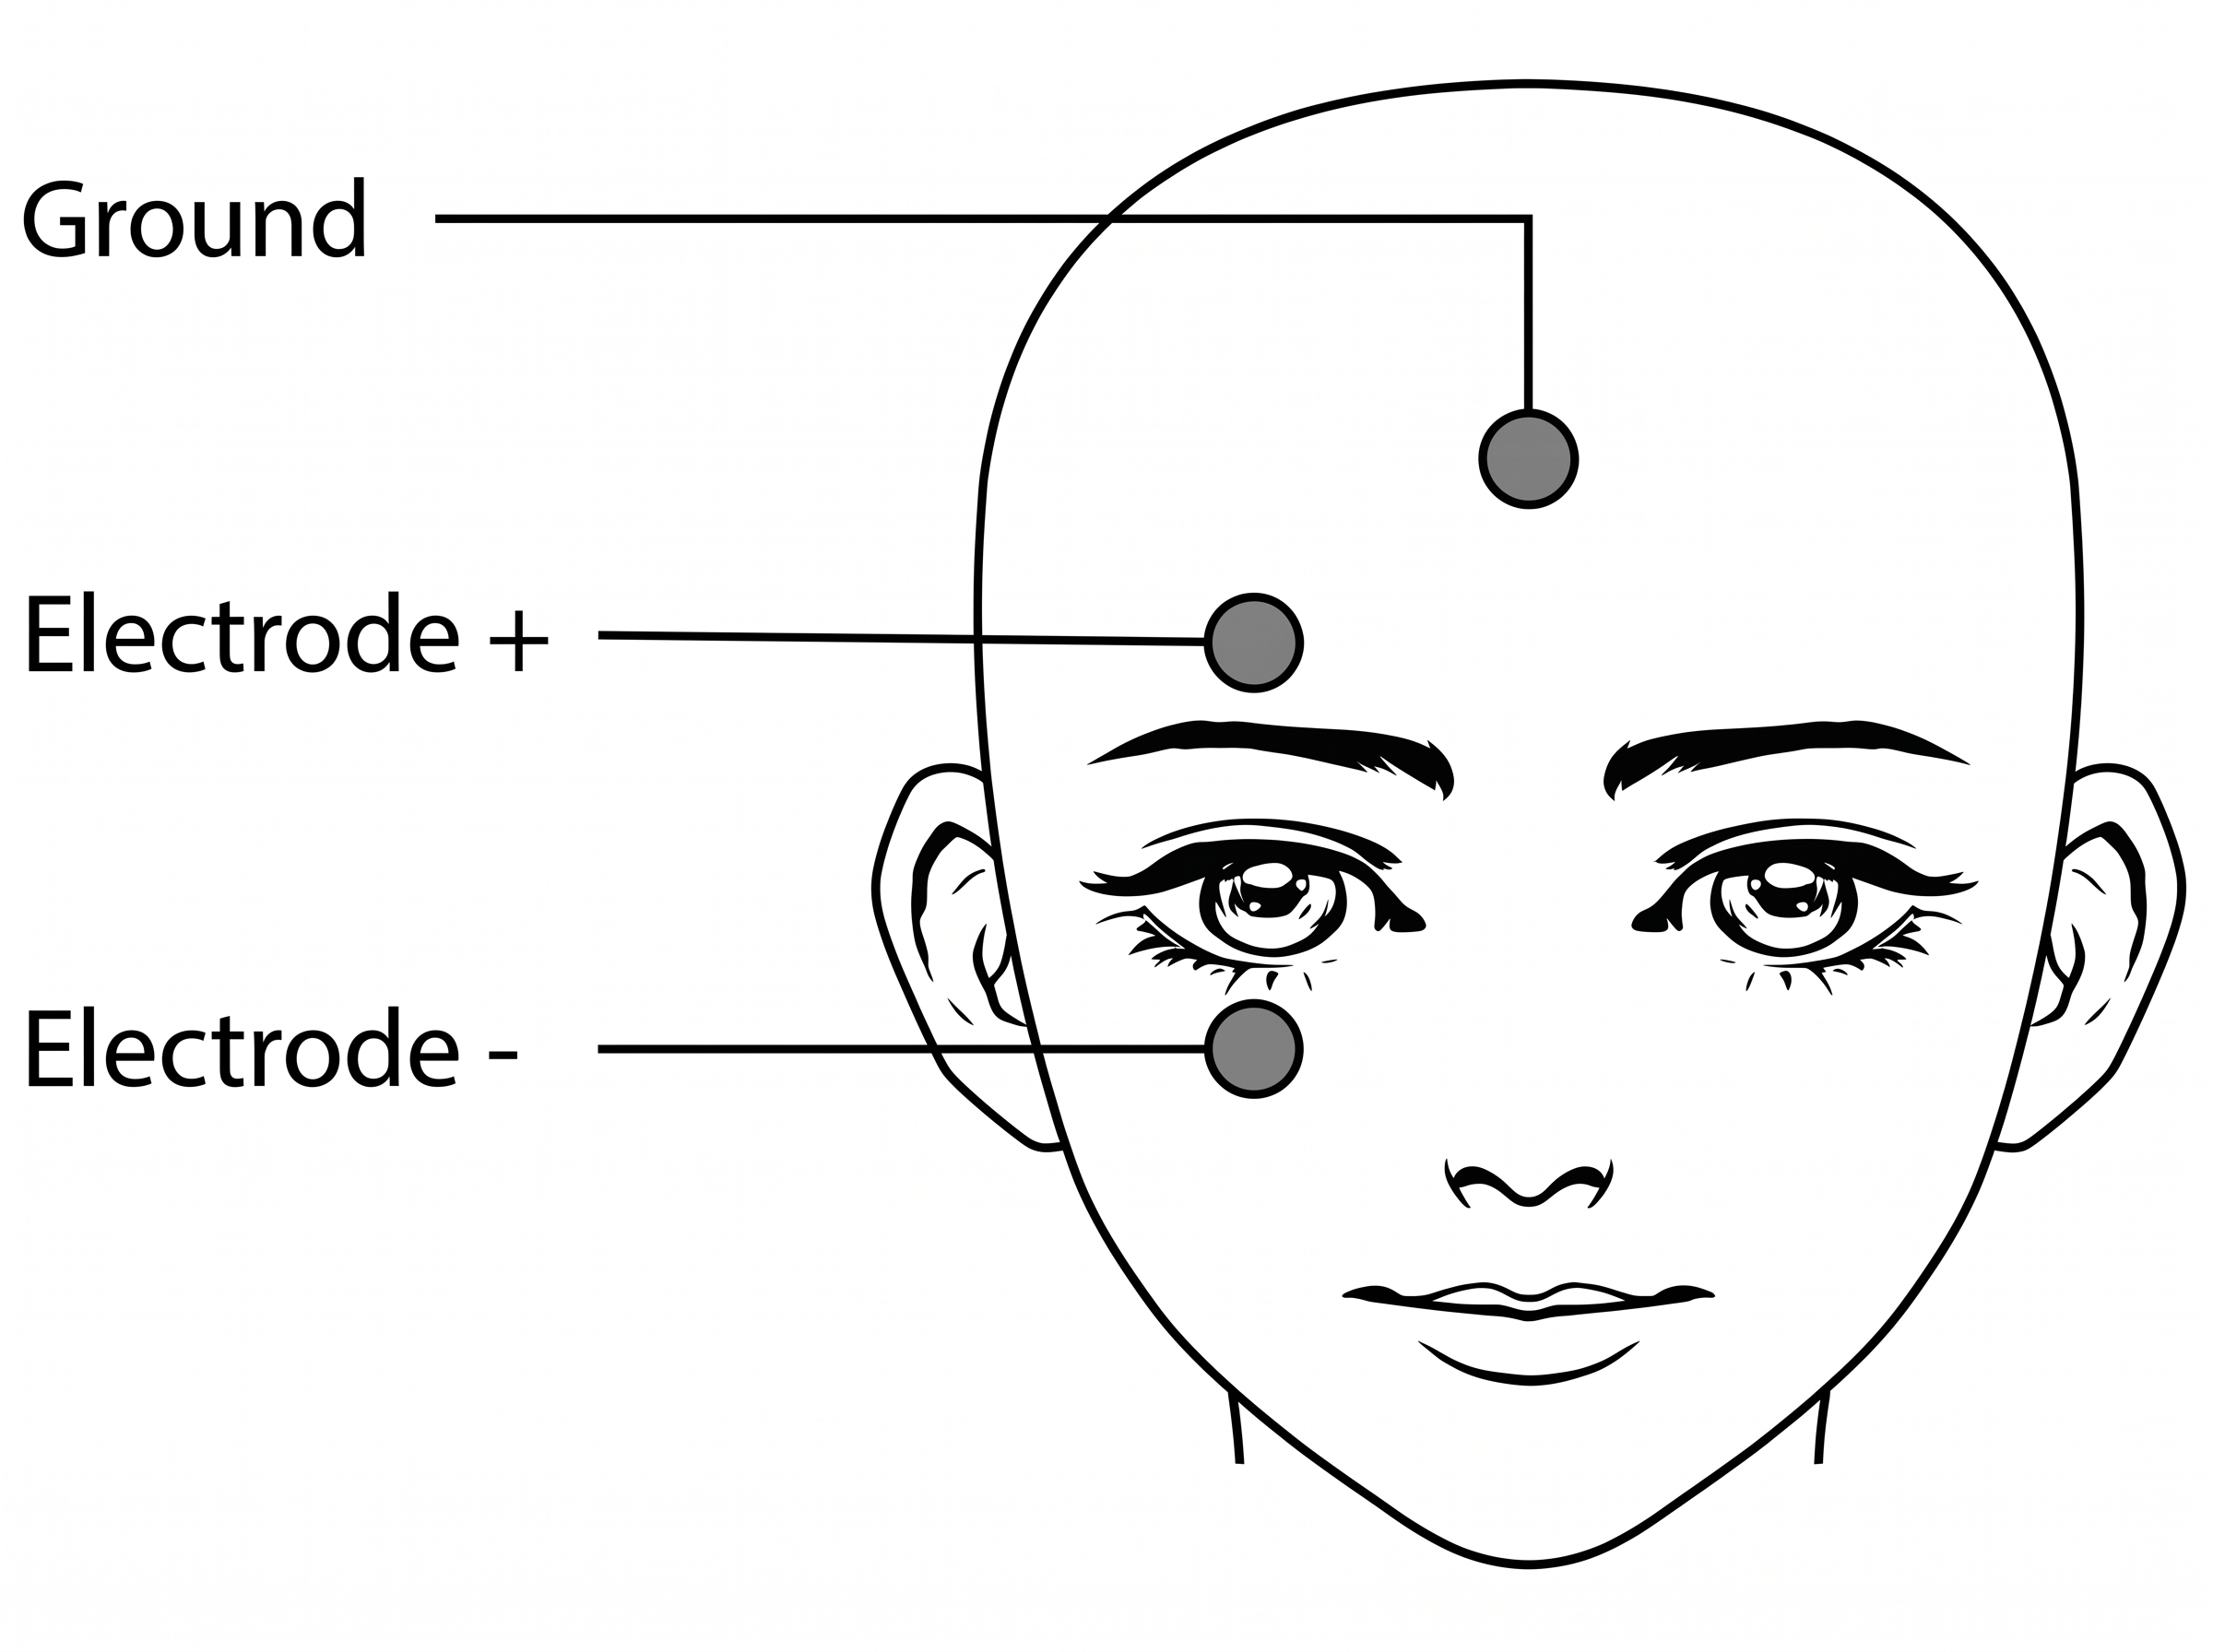
\includegraphics[width=0.6\textwidth]{vertical_eog_electrode_placement.jpeg}
  \caption{Vertical EOG electrode placement \cite{li2021evaluation}.}
  \label{fig:vertical_eog_placement}
\end{figure}

\FloatBarrier
\subsection{Pathophysiology of Target Neuromuscular Disorders}
\label{subsec:target_disorders}

The developed assistive platform is designed for individuals suffering from severe neuromuscular impairment and loss of voluntary motor control. Key target pathologies include Amyotrophic Lateral Sclerosis (ALS), a progressive neurodegenerative disease; Quadriplegia, resulting in total limb paralysis; and Locked-in Syndrome (LIS), where cognitive awareness remains intact despite voluntary muscle loss. Furthermore, the system targets patients with Muscular Dystrophy (MD), a group of diseases causing progressive muscular weakness. In many stages of MD, the extraocular muscle control remains relatively preserved, making EOG an optimal, non-fatiguing physiological pathway for human-machine interaction \cite{hall2016guyton}.

\FloatBarrier
\subsection{Clinical Justification for EOG-Based Human-Machine Interfaces}
\label{subsec:clinical_justification}

The medical justification for selecting EOG signals as a control medium for these patient populations relies on an important anatomical and neurological principle: the cranial nerves responsible for extraocular muscle control—specifically the oculomotor nerve (CN III), trochlear nerve (CN IV), and abducens nerve (CN VI)—are typically spared during the progression of neurodegenerative conditions like ALS and severe paralysis \cite{hall2016guyton}. Because ocular motility remains functionally preserved, voluntary eye movements represent a reliable, non-fatiguing physiological pathway through which severely impaired patients can interact with human-machine interfaces (HMIs) to regain independence in mobility and communication.

% ============================================================
% Section 2.2: Engineering Background
% ============================================================
\section{Engineering Background}
\label{sec:engineering_background}

Designing an EOG-guided 3D-printed prototype wheelchair and virtual speller system requires integrating bio-instrumentation, analog electronics, digital signal processing, embedded control, and distance sensing.

\FloatBarrier
\subsection{Principles of Bio-Signal Acquisition and Ambient Noise}
\label{subsec:biopotential_acquisition}

Acquiring electrooculography (EOG) signals from the skin surface requires overcoming several physical and electrical challenges. First, high skin-electrode interface impedance significantly attenuates the microvolt-level biological signal. Second, the bio-potential is highly susceptible to ambient electromagnetic interference, primarily $50\,\text{Hz}$ power line noise, which the human body picks up like an antenna and presents as a common-mode voltage across the measurement electrodes. Additionally, motion artifacts resulting from lead wire movement or adjacent electromyographic (EMG) muscle contractions contaminate the raw signal \cite{webster2009medical}. Overcoming these acquisition challenges requires designing a front-end amplifier with high input impedance ($>10^9\,\Omega$) and high common-mode rejection ratio ($\text{CMRR} > 100\,\text{dB}$) prior to any digital processing stage. To visualize the severity of these noise contamination sources, Figure \ref{fig:eog_noise_comparison} presents a conceptual comparison between a raw EOG signal corrupted by 50 Hz interference and baseline drift versus the ideal clean blink waveform that the signal conditioning chain aims to recover.

\begin{figure}[H]
  \centering
  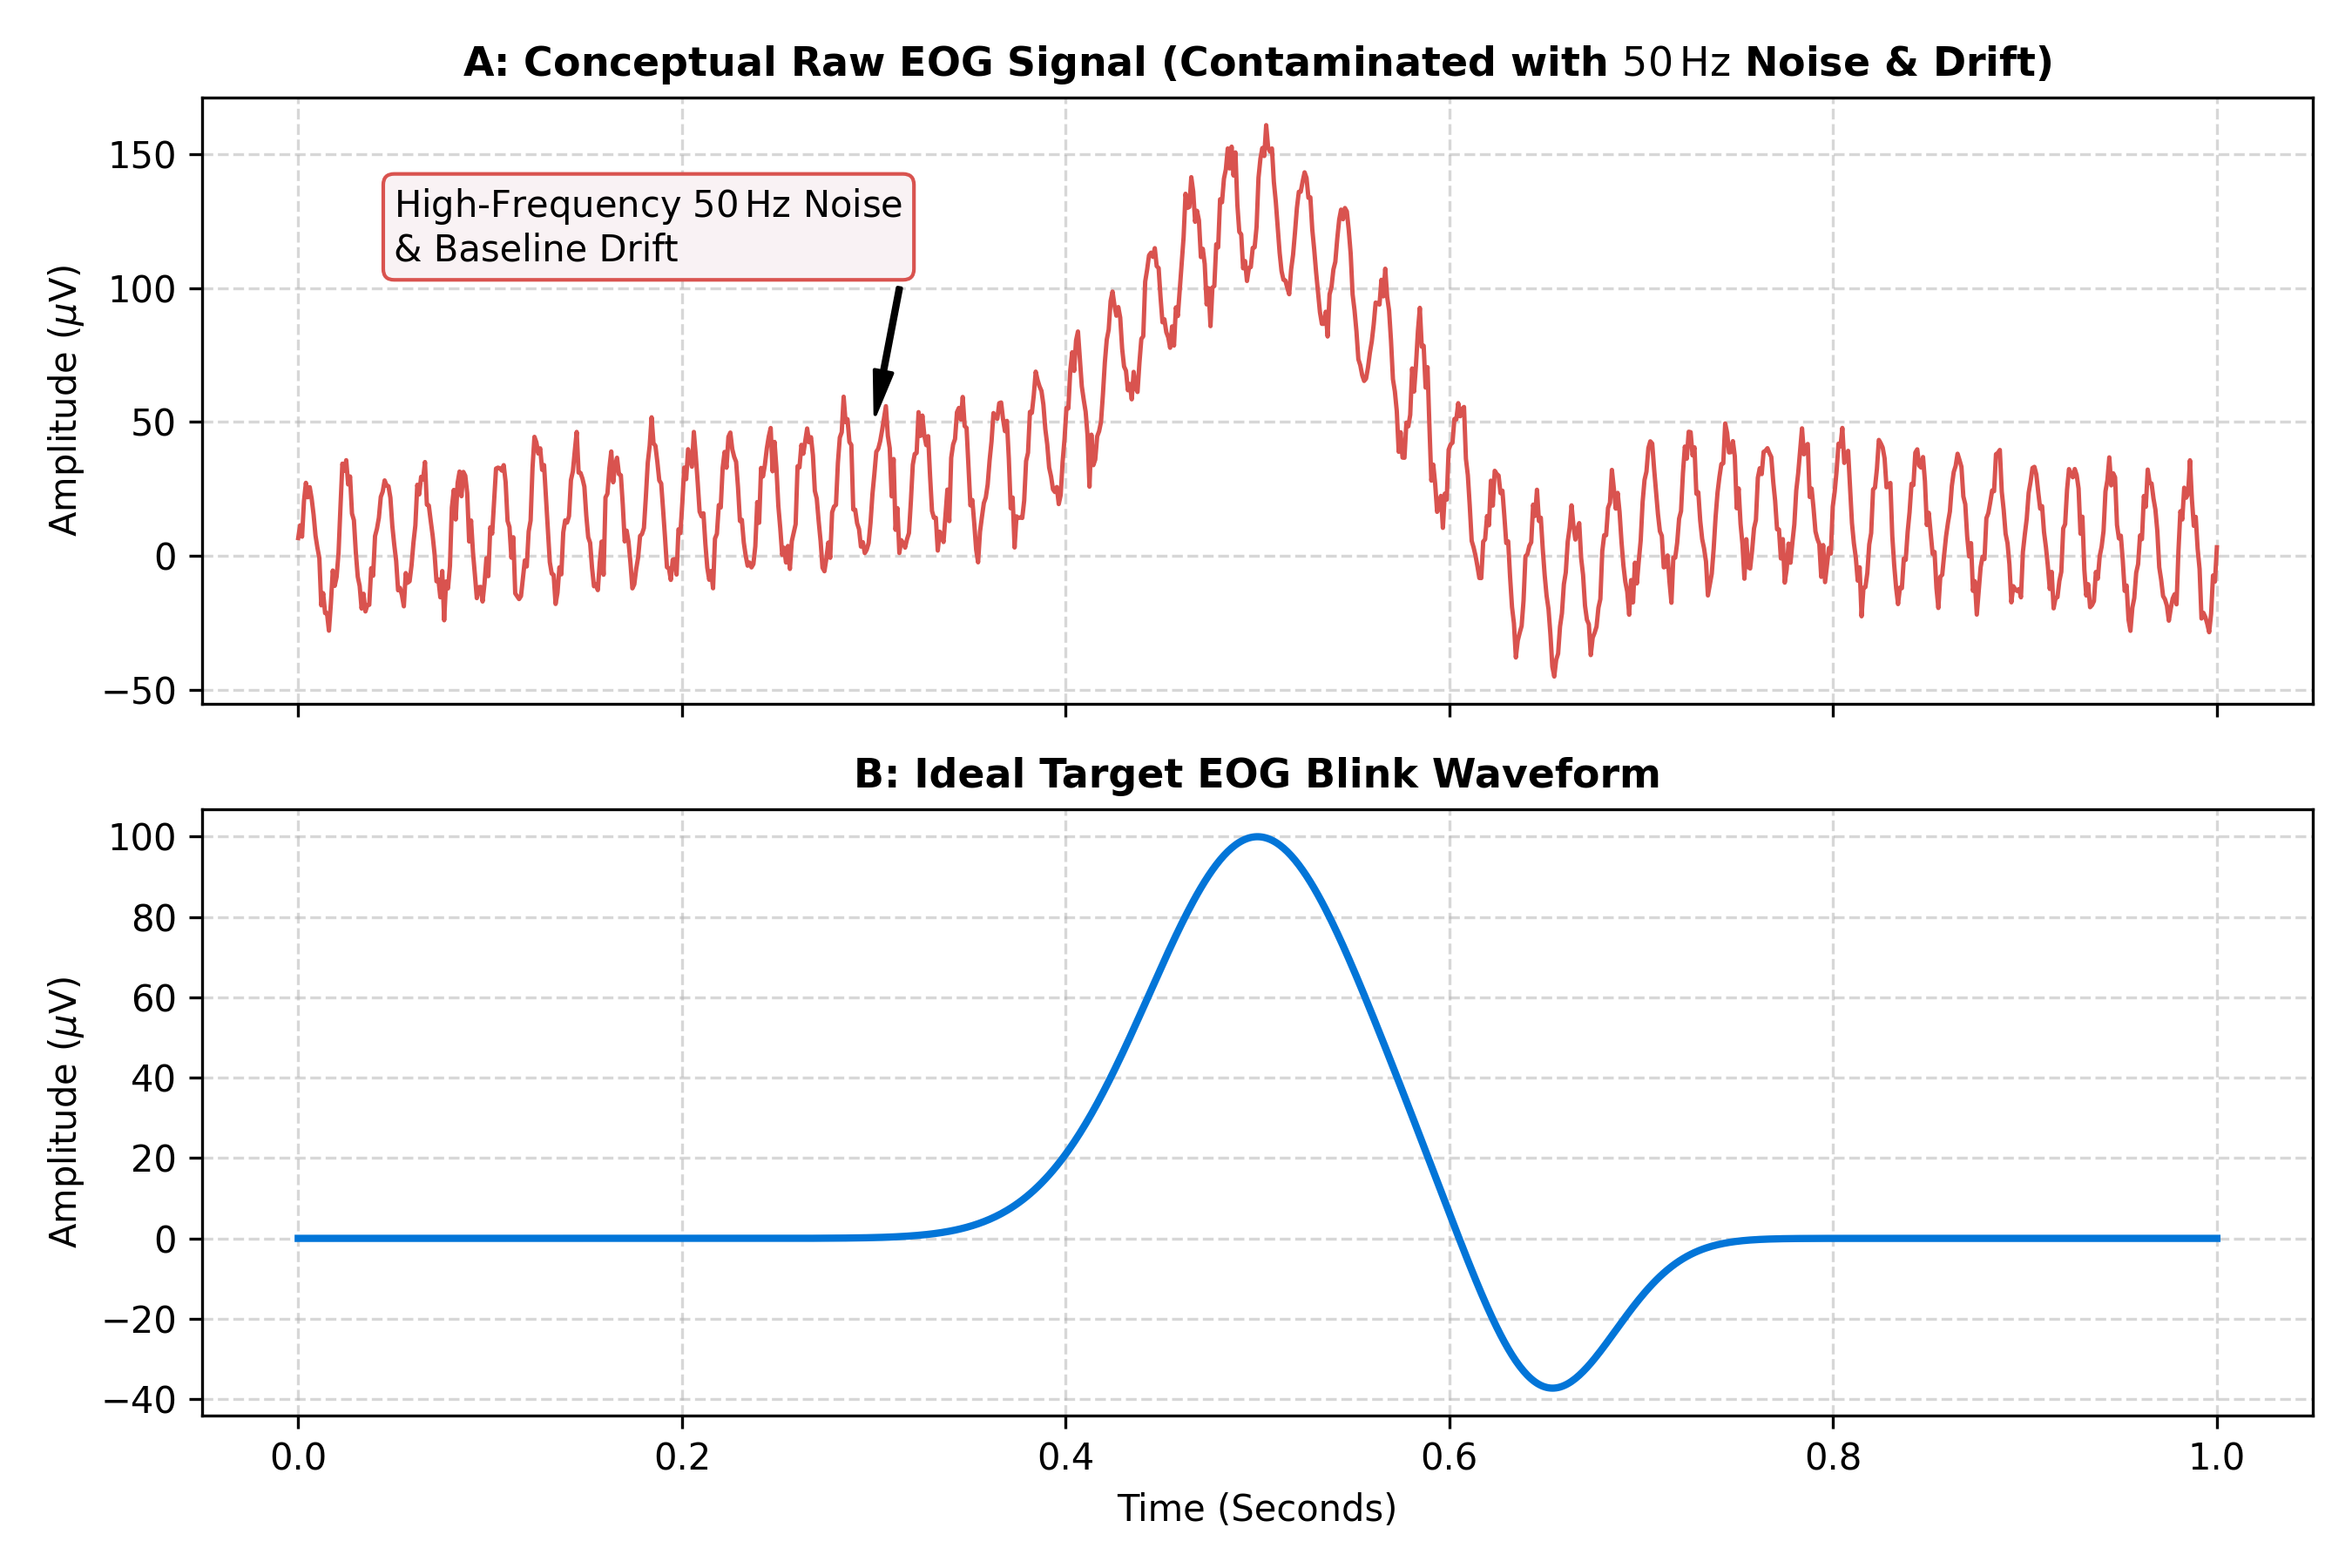
\includegraphics[width=0.9\textwidth]{eog_noise_comparison.png}
  \caption{Conceptual comparison between an ideal clean EOG blink transient and a raw bio-signal contaminated with 50 Hz power-line interference and baseline drift.}
  \label{fig:eog_noise_comparison}
\end{figure}

\FloatBarrier
\subsection{Instrumentation Amplifiers and the Significance of CMRR}
\label{subsec:instrumentation_amp_cmrr}

To isolate weak bio-potentials from severe ambient interference, an instrumentation amplifier (InAmp) is utilized in the primary acquisition stage rather than standard operational amplifiers (Op-Amps). An instrumentation amplifier operates on differential amplification principles; it amplifies the minute differential voltage existing between two measurement electrodes (representing ocular displacement) while virtually rejecting the common-mode potential present identically at both electrodes (such as $50\,\text{Hz}$ power line noise) \cite{webster2009medical}.

The efficiency of an amplifier in suppressing common-mode noise is mathematically defined by the Common-Mode Rejection Ratio ($\text{CMRR}$), expressed in decibels ($\text{dB}$) as:
\begin{equation}
\text{CMRR (dB)} = 20 \log_{10} \left( \frac{A_d}{A_{cm}} \right)
\label{eq:cmrr_formula}
\end{equation}
where $A_d$ represents the differential voltage gain and $A_{cm}$ represents the common-mode voltage gain.

In precision biomedical applications such as EOG acquisition, maintaining a high $\text{CMRR}$ is essential to ensure signal integrity. This engineering requirement justifies selecting the AD620 integrated circuit (IC) for the primary pre-amplification stage in this project's hardware design. The AD620 provides an exceptionally high input impedance and a minimum $\text{CMRR}$ of $100\,\text{dB}$ \cite{ad620datasheet}.

In addition to noise rejection capabilities, the AD620 instrumentation amplifier allows precise control over the differential voltage gain ($G$) using a single external resistor ($R_G$), governed by the manufacturer's characteristic transfer equation \cite{ad620datasheet}:
\begin{equation}
G = 1 + \frac{49.4\,\text{k}\Omega}{R_G}
\label{eq:ad620_transfer}
\end{equation}
This adjustable feature offers necessary engineering flexibility to achieve the target preliminary amplification for weak blink transients prior to passing the signal through subsequent active filtering stages. To illustrate this integrated architecture, Figure \ref{fig:ad620_functional_schematic} depicts the internal functional schematic of the AD620 instrumentation amplifier and the external connection of the gain-setting resistor ($R_G$) across Pins 1 and 8 \cite{ad620datasheet}.

\begin{figure}[H]
  \centering
  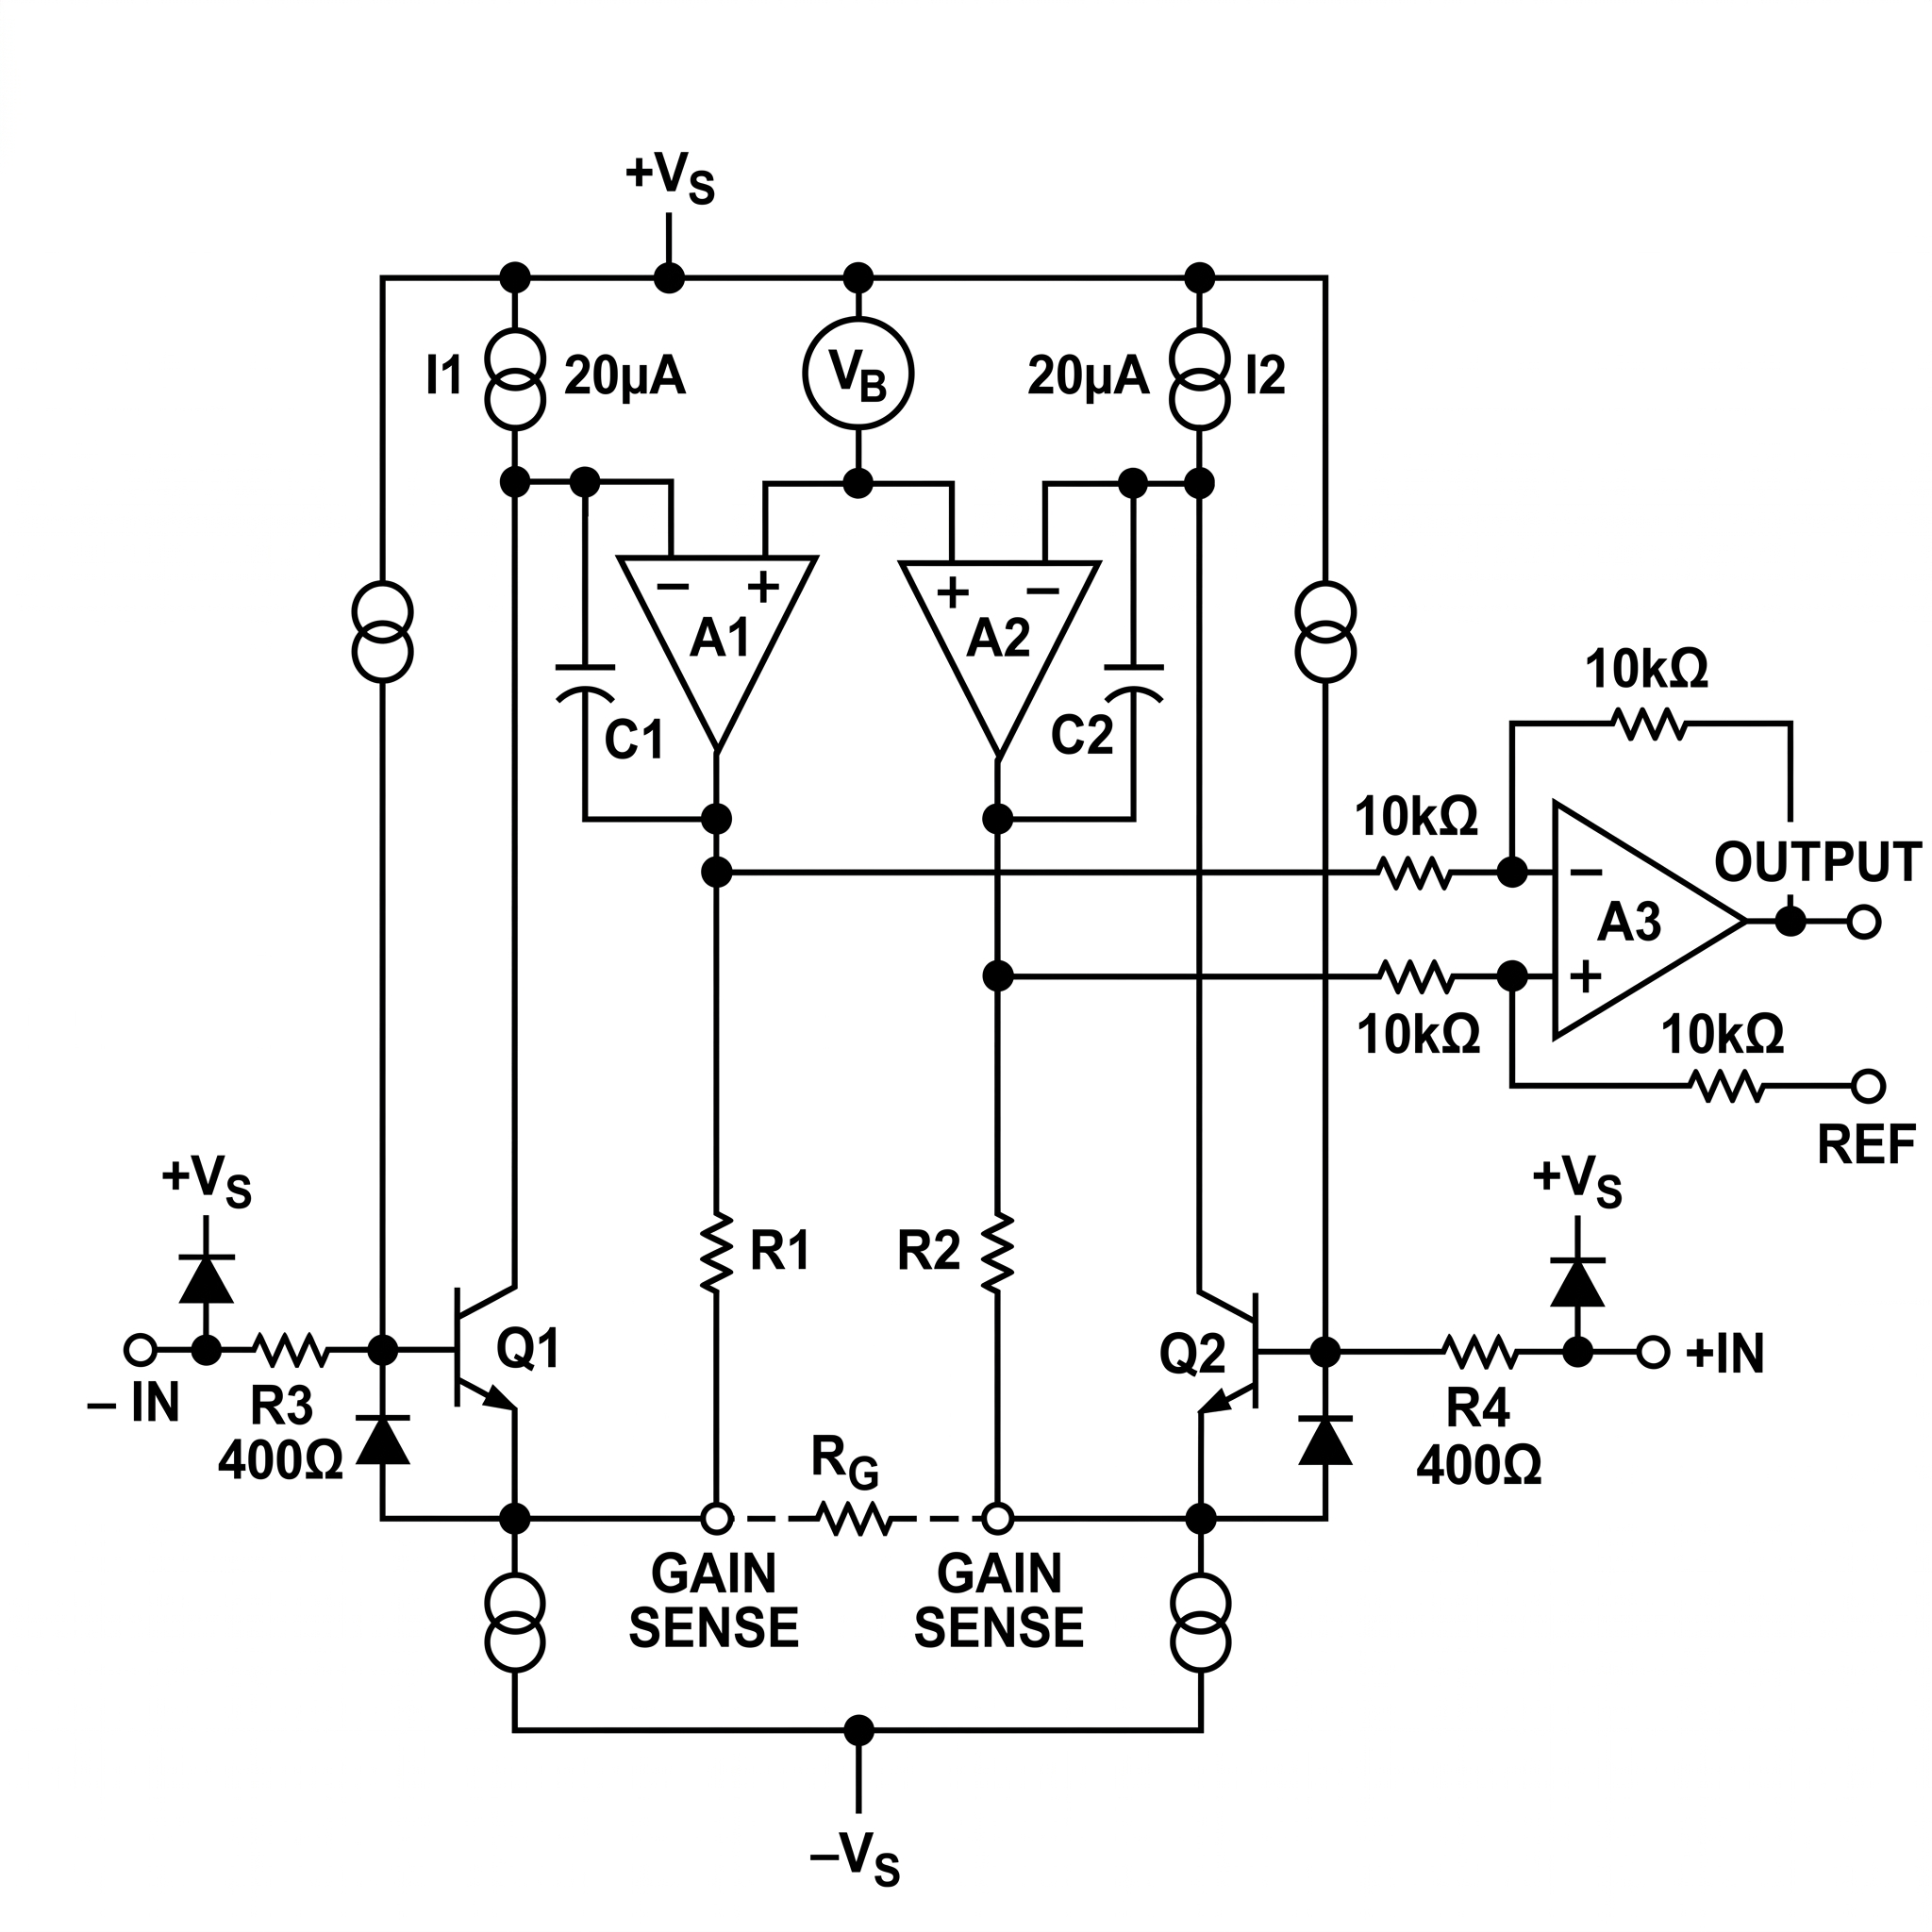
\includegraphics[width=0.65\textwidth]{ad620.jpeg}
  \caption{Functional architecture and $R_G$ gain-setting connection of the AD620 InAmp \cite{ad620datasheet}.}
  \label{fig:ad620_functional_schematic}
\end{figure}

\FloatBarrier
\subsection{Active Analog Filters (Active Sallen-Key and Notch Filters)}
\label{subsec:active_analog_filters}

Active analog filters are critical for conditioning acquired bio-potentials prior to analog-to-digital conversion. Active topologies incorporating operational amplifiers are preferred in low-frequency biomedical applications because they eliminate the need for bulky inductors and offer low output impedance, which prevents inter-stage loading effects \cite{webster2009medical}.

The Sallen-Key architecture is one of the most widely implemented topologies for designing second-order low-pass and high-pass filters. Assuming equal component values ($R_1 = R_2 = R$ and $C_1 = C_2 = C$), the cut-off frequency ($f_c$) is governed by:
\begin{equation}
f_c = \frac{1}{2 \pi R C}
\label{eq:sallen_key_fc_bg}
\end{equation}

In biomedical signal processing, a high-pass filter (HPF) removes the DC offset caused by half-cell potentials at the skin-electrode interface, whereas a low-pass filter (LPF) restricts the signal bandwidth to satisfy sampling requirements and prevent aliasing. Furthermore, to eliminate $50\,\text{Hz}$ or $60\,\text{Hz}$ power-line interference, a notch filter (band-stop filter) is incorporated to sharply attenuate the specific power line frequency without distorting the primary biophysical spectrum. To visualize the spectral selectivity of these conditioning stages, Figure \ref{fig:active_filters_bode} illustrates the frequency response characteristics (Bode plots) of the high-pass ($f_c = 0.8\,\text{Hz}$), low-pass ($f_c = 30\,\text{Hz}$), and 50 Hz notch filters \cite{webster2009medical}.

\begin{figure}[H]
    \centering
    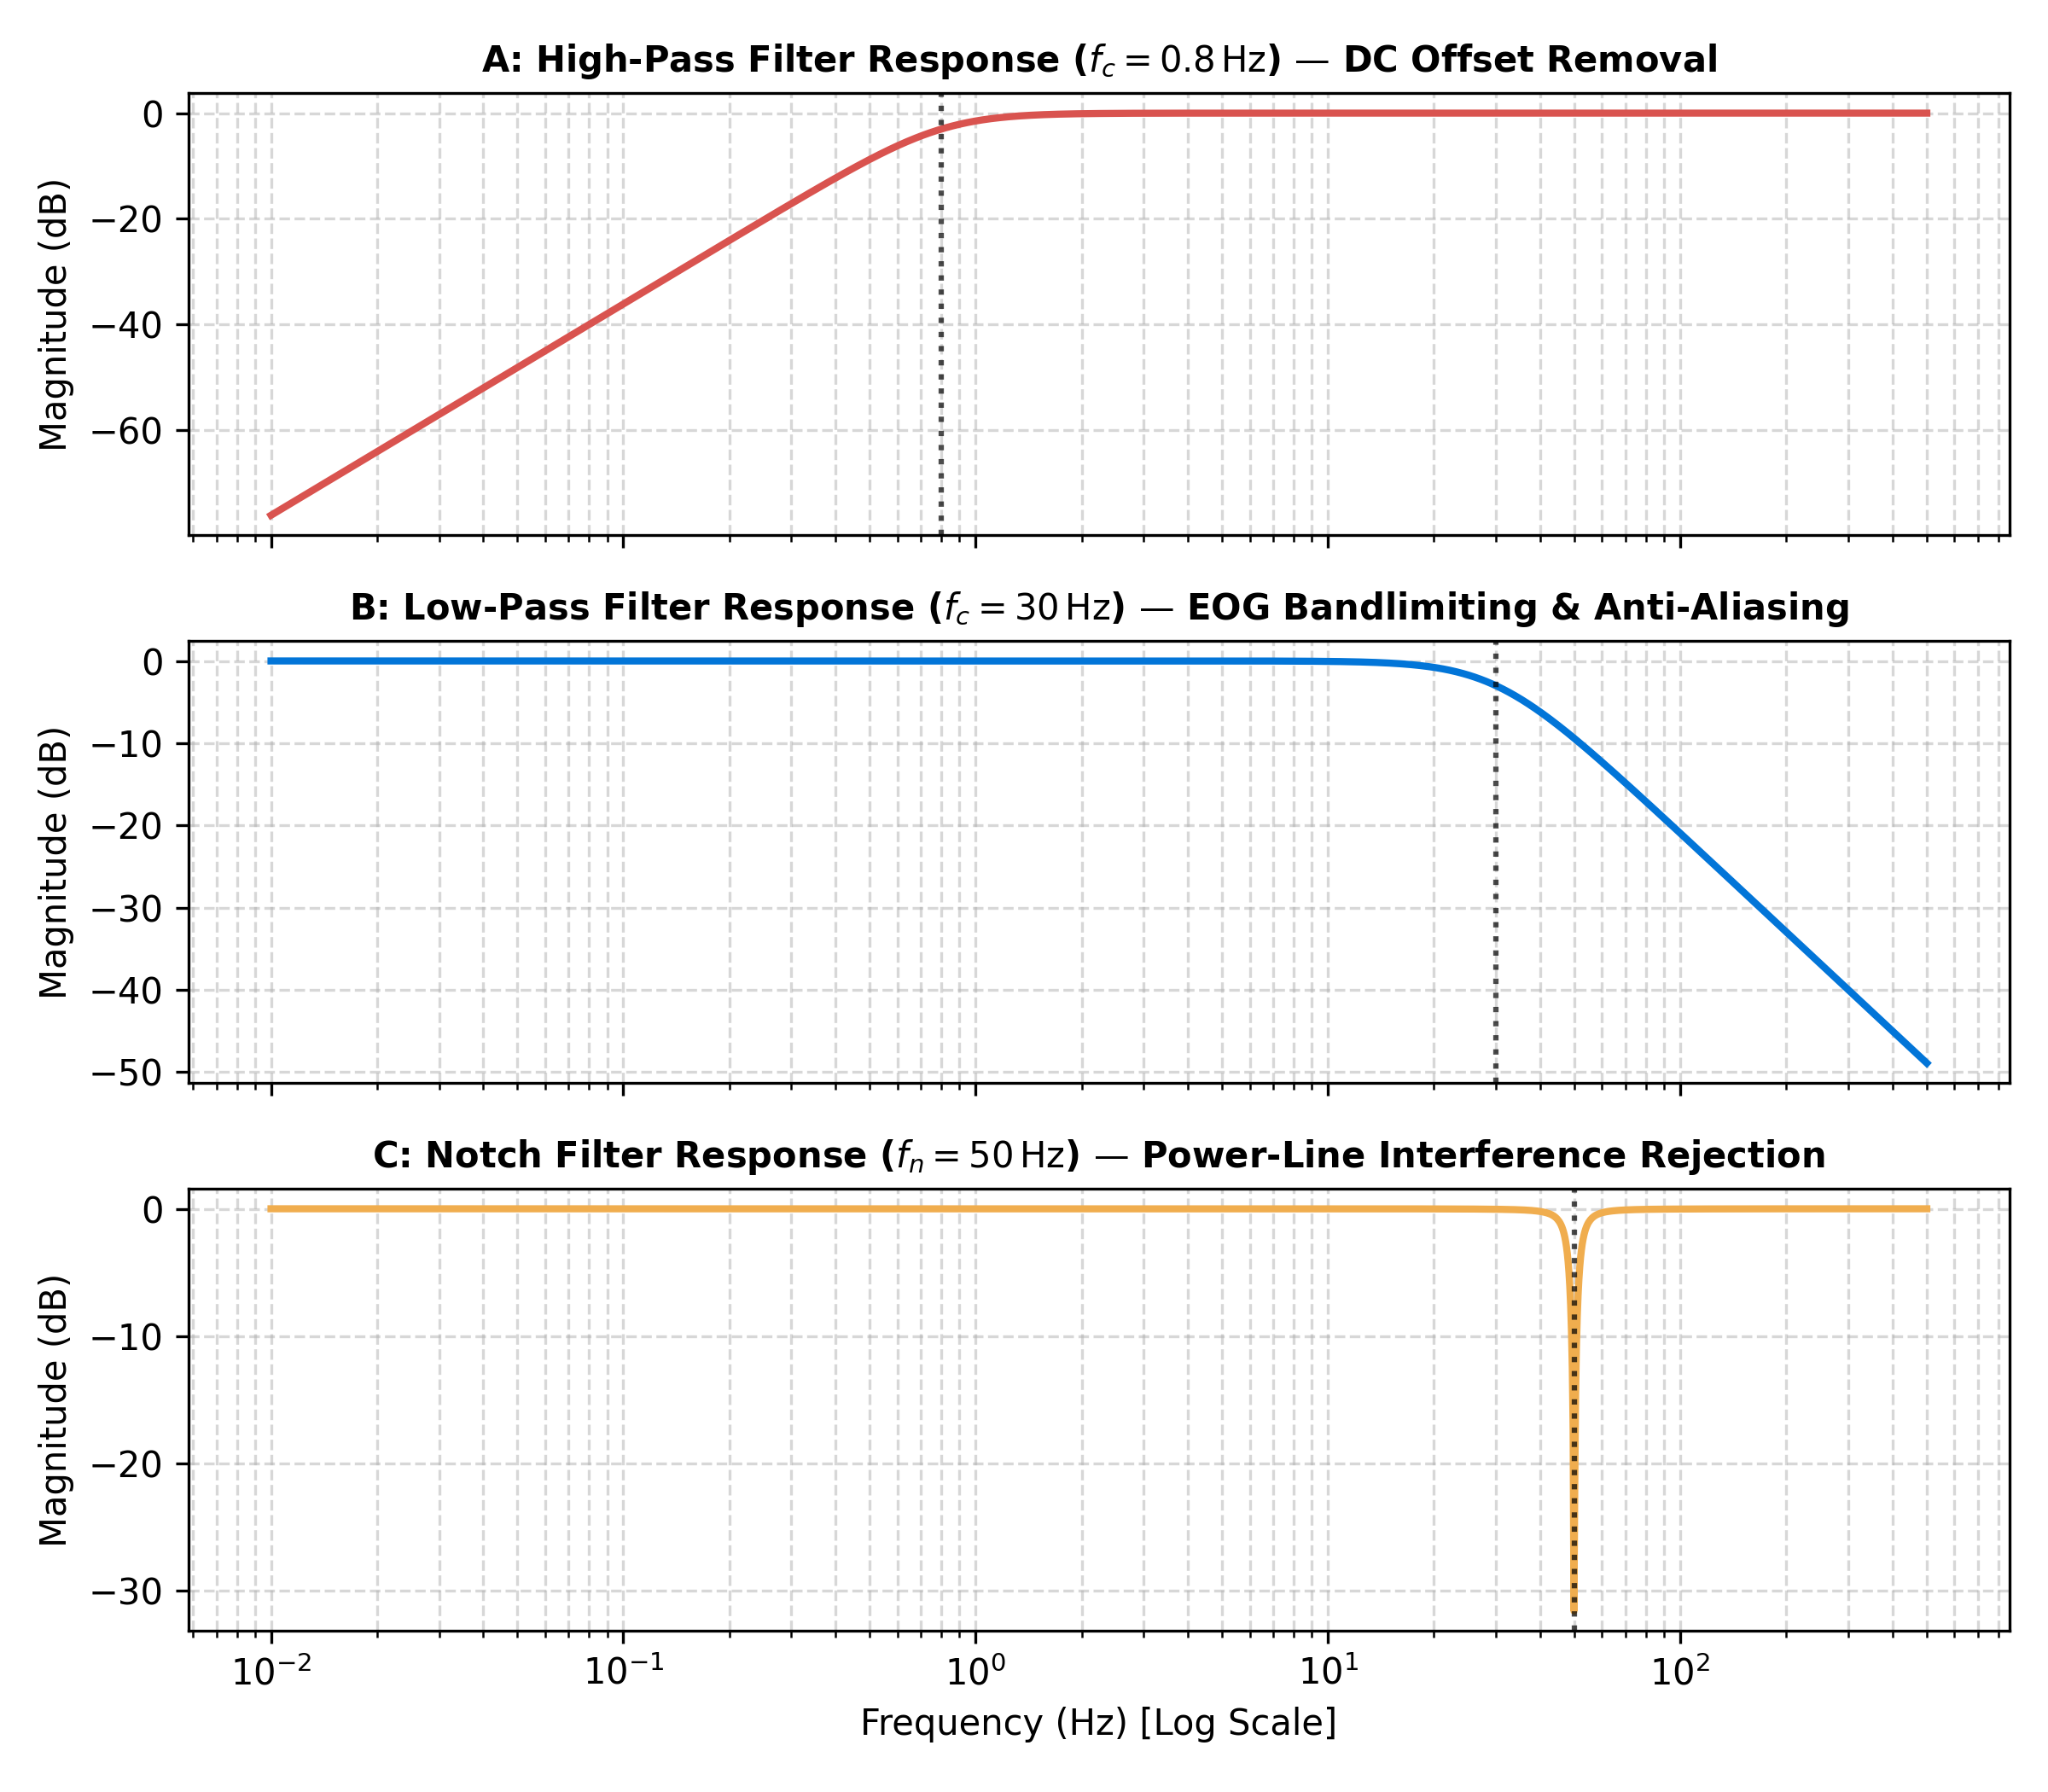
\includegraphics[width=0.65\textwidth]{Active_Filters_EOG_30Hz.png}
    \caption{Ideal frequency response curves (Bode plots) for High-Pass ($f_c = 0.8\,\text{Hz}$), Low-Pass ($f_c = 30\,\text{Hz}$), and 50 Hz Notch active filters in EOG signal conditioning \cite{webster2009medical}.}
    \label{fig:active_filters_bode}
\end{figure}

\FloatBarrier
\subsection{Digital Signal Processing and Pattern Extraction}
\label{subsec:dsp_moving_average}

Once digitized by an Analog-to-Digital Converter (ADC) at a sampling rate adhering to the Nyquist-Shannon sampling theorem, raw bio-signals undergo digital processing to enhance signal quality and extract feature metrics. Processing typically begins with digital smoothing techniques, such as moving average filtering, to suppress high-frequency ripple components and highlight primary signal morphology.

Pattern extraction primarily relies on threshold detection algorithms. Mathematically, the instantaneous discrete signal sample $x(n)$ is compared against a predefined threshold value $Th$. When $x(n) > Th$, the event onset is logged. To differentiate between distinct physiological patterns (such as involuntary vs. intentional blinks), the algorithm measures the elapsed pulse width ($T_{\text{width}}$) during which the signal remains above the threshold. Based on this temporal width and event frequency, the signal is classified to generate real-time control commands for external hardware. To demonstrate this temporal feature extraction logic, Figure \ref{fig:eog_threshold_twidth} depicts the threshold crossing criterion $x(n) > Th$ and the measurement of pulse width ($T_{\text{width}}$) used for pattern classification.

\begin{figure}[H]
    \centering
    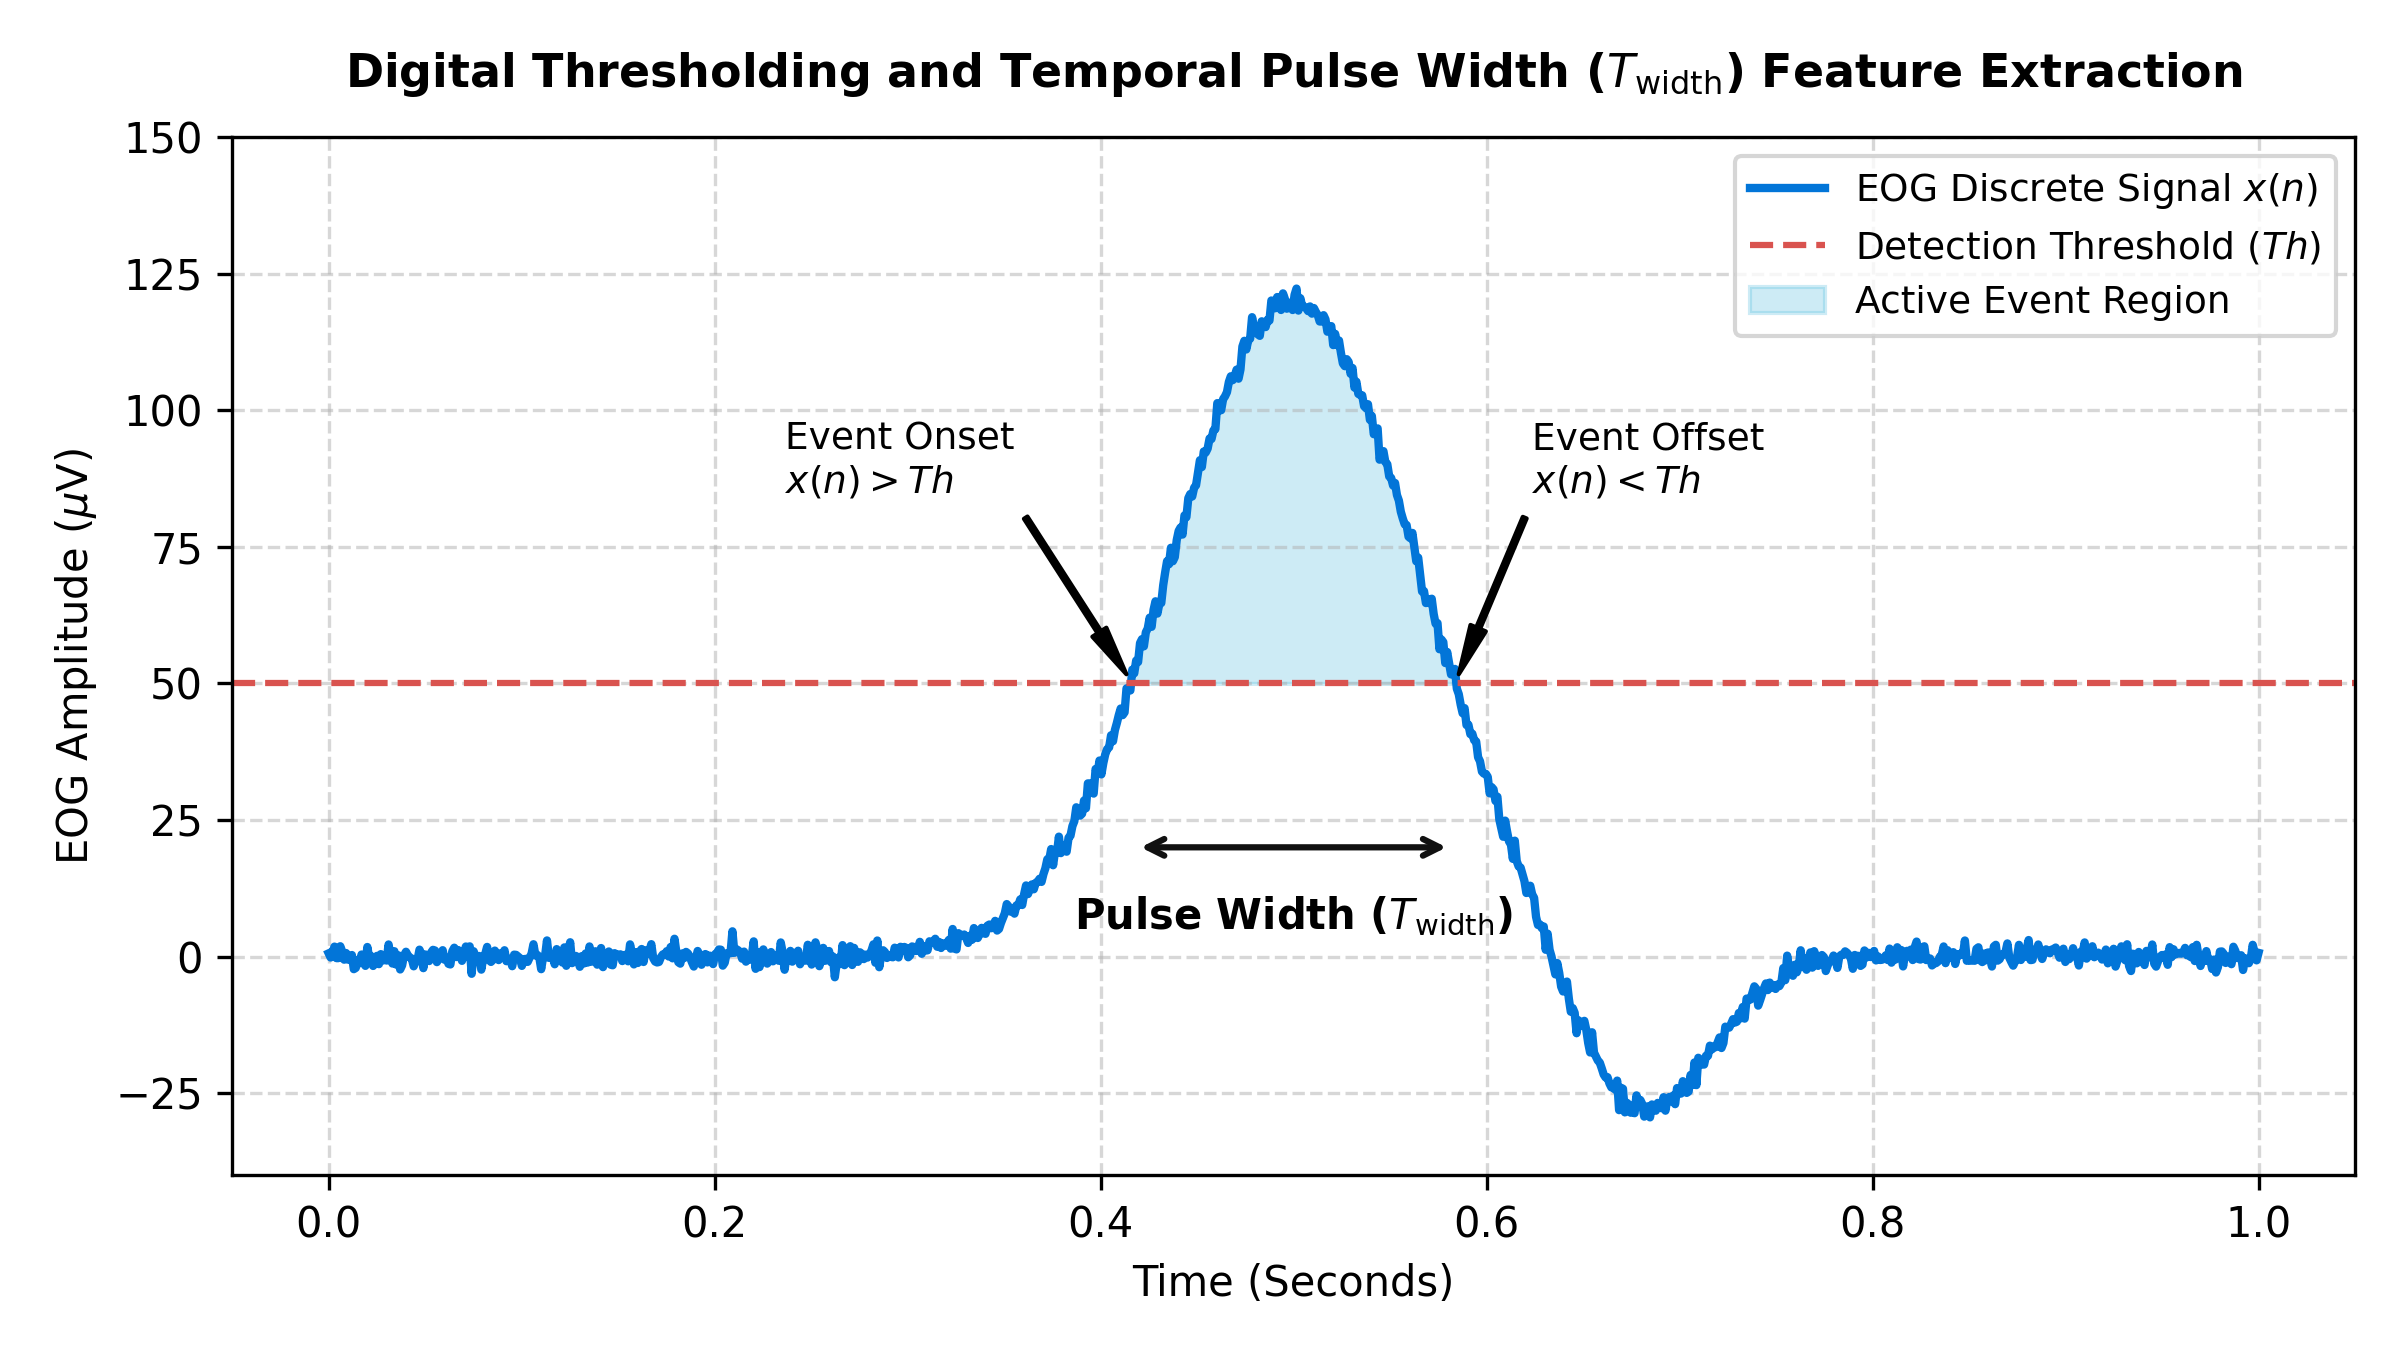
\includegraphics[width=0.65\textwidth]{EOG_Threshold_Twidth.png}
    \caption{Conceptual digital thresholding scheme and temporal pulse width ($T_{\text{width}}$) feature extraction for EOG event classification.}
    \label{fig:eog_threshold_twidth}
\end{figure}

\FloatBarrier
\subsection{Motor Control and Pulse-Width Modulation (PWM)}
\label{subsec:dc_motor_pwm}

Guiding robotic and mobility systems requires precise control over both the rotational speed and direction of direct current (DC) motors. Because microcontrollers cannot directly deliver the high currents required by DC motors, motor driver circuits act as high-current electronic switches interfacing the controller to the motor power supply.

To regulate motor speed efficiently, Pulse-Width Modulation (PWM) is employed. PWM rapidly switches the applied voltage between ON and OFF states at a fixed switching frequency. The ratio of the ON duration to the total period, known as the duty cycle ($D$), determines the effective average output voltage ($V_{\text{out}}$) applied to the motor:
\begin{equation}
V_{\text{out}} = D \times V_{\text{in}}
\label{eq:pwm_vout}
\end{equation}
where $V_{\text{in}}$ represents the supply voltage. The duty cycle $D$ is calculated as a percentage:
\begin{equation}
D = \frac{T_{\text{on}}}{T_{\text{total}}} \times 100\%
\label{eq:pwm_duty_cycle}
\end{equation}
where $T_{\text{on}}$ is the active pulse duration and $T_{\text{total}}$ is the total period ($T_{\text{on}} + T_{\text{off}}$). This technique delivers linear speed control while minimizing thermal power dissipation. To illustrate the relationship between pulse active time and effective voltage, Figure \ref{fig:pwm_duty_cycles} compares PWM pulse trains at different duty cycles and their resulting average output voltages.

\begin{figure}[H]
    \centering
    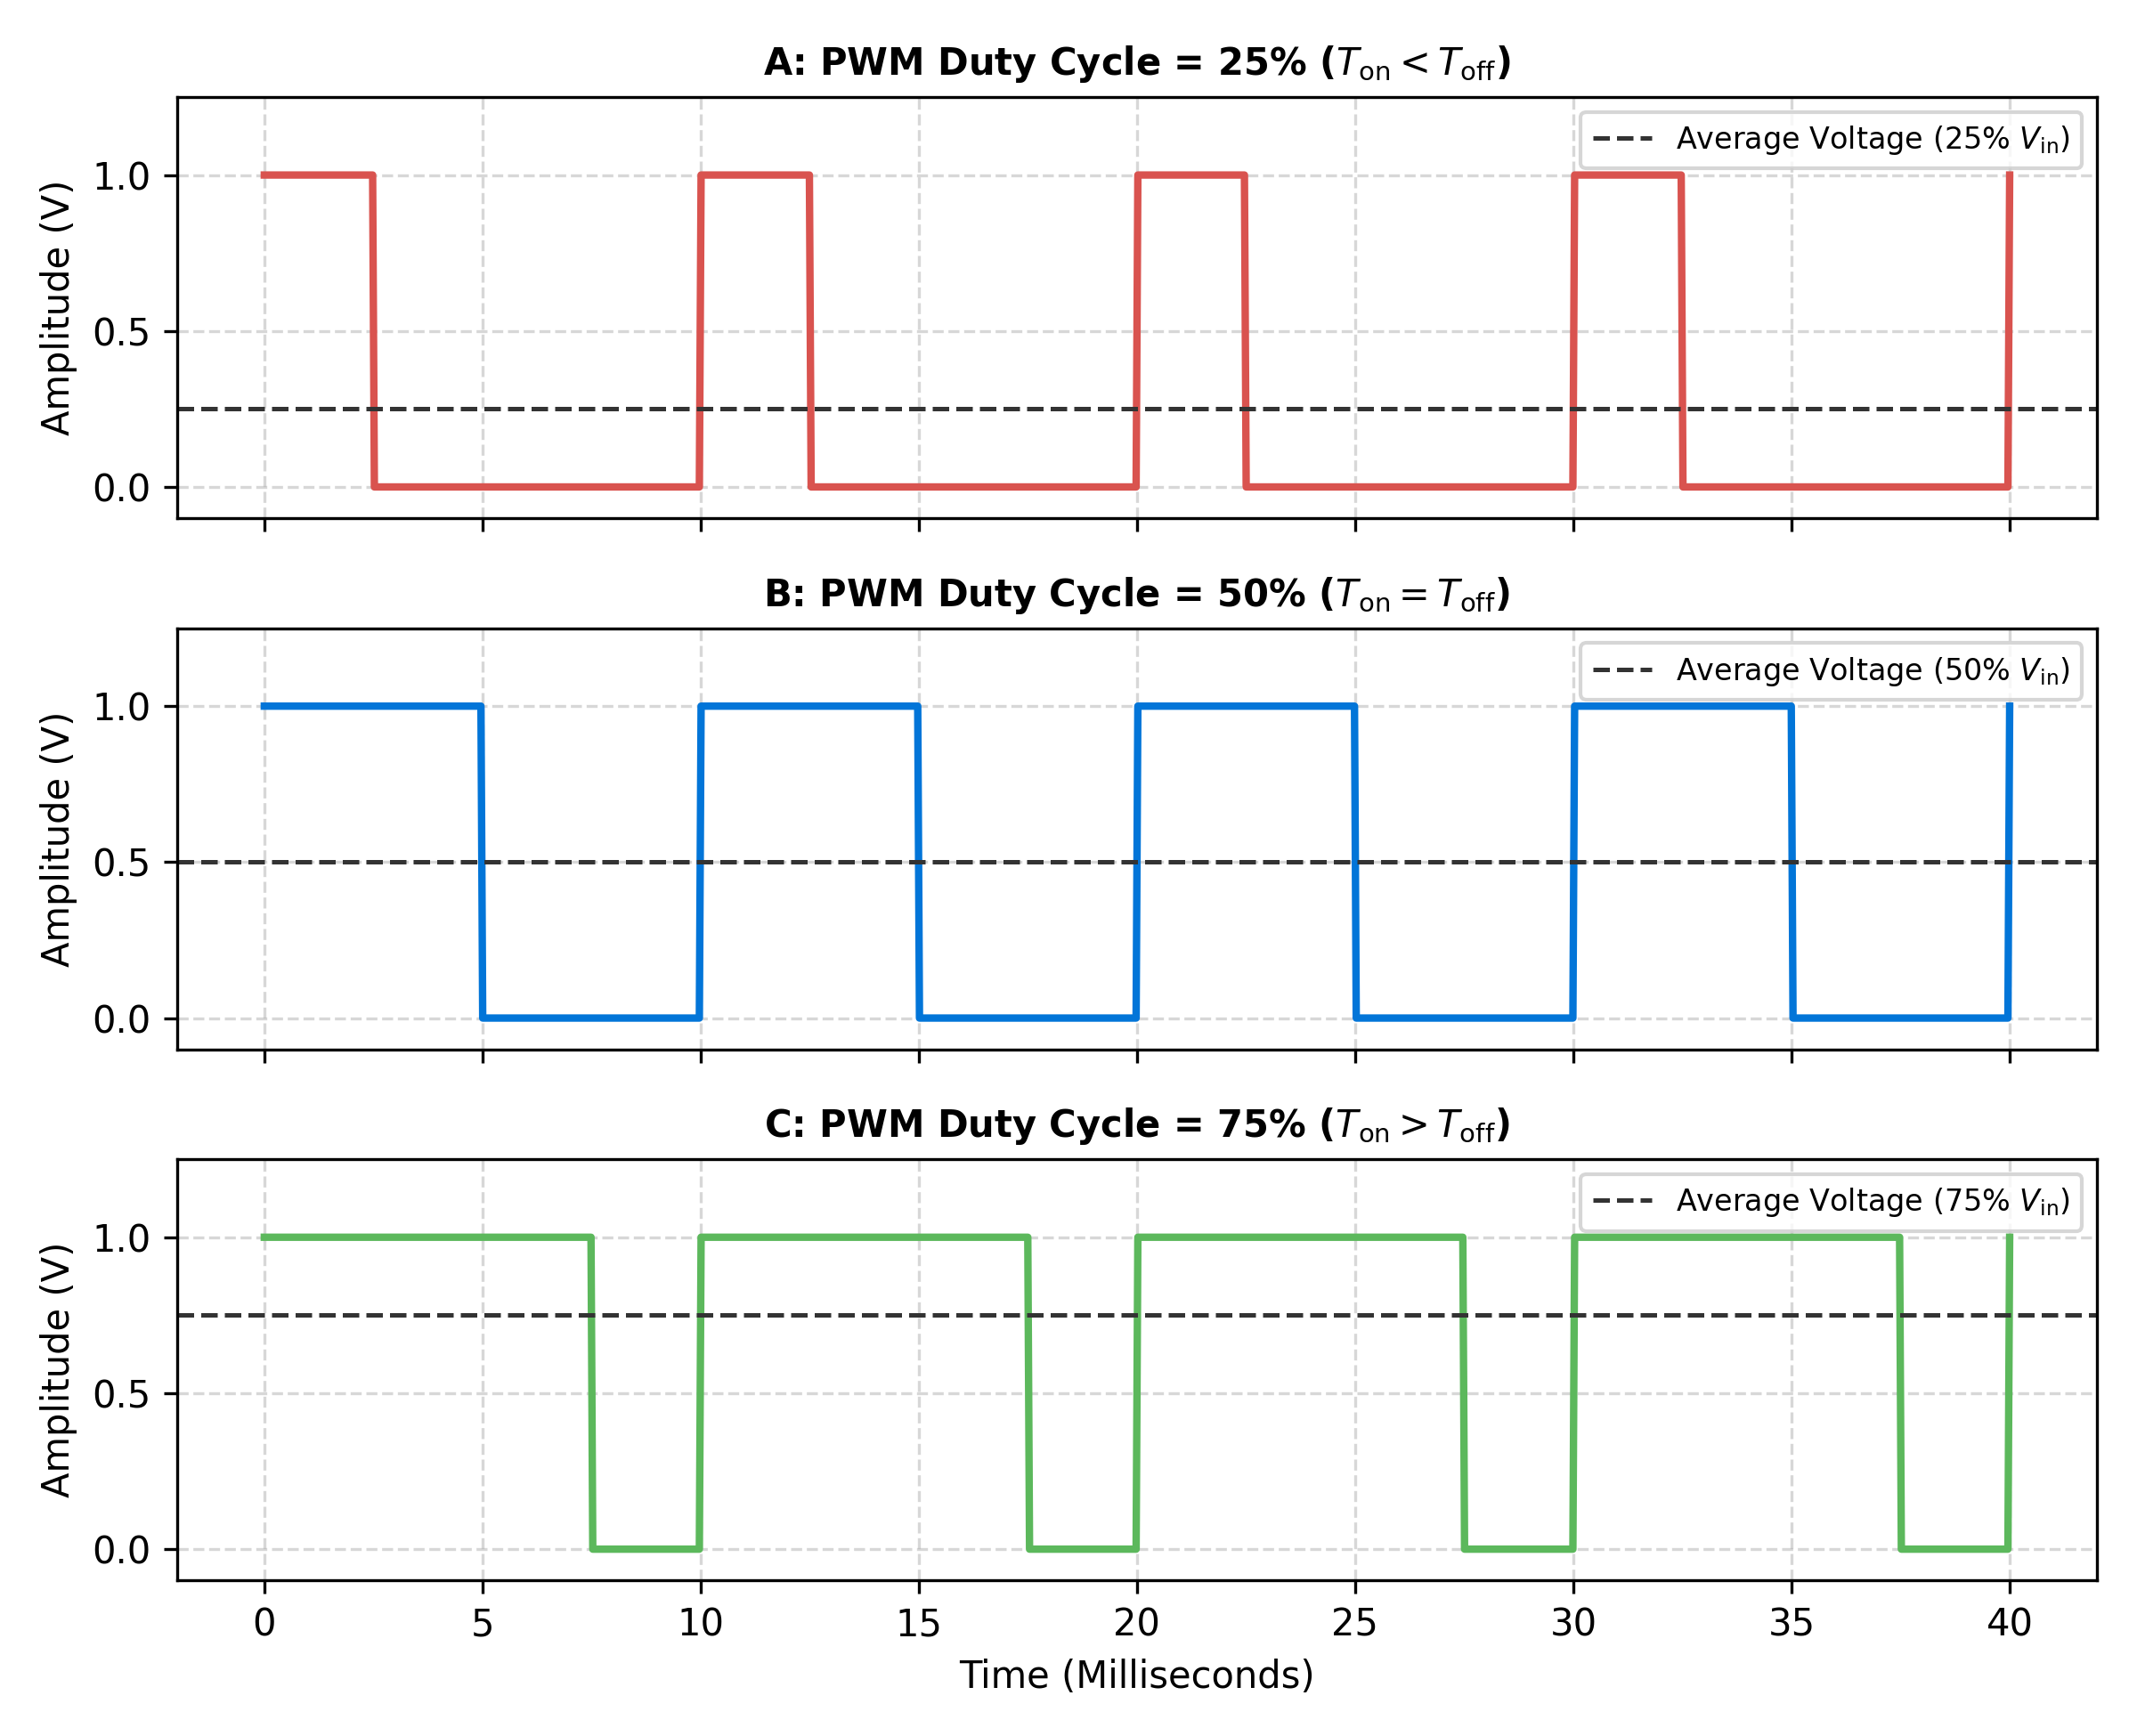
\includegraphics[width=0.65\textwidth]{PWM_Duty_Cycles_Comparison.png}
    \caption{Pulse-Width Modulation (PWM) pulse trains at various duty cycles ($25\%$, $50\%$, and $75\%$) and their corresponding average output voltages.}
    \label{fig:pwm_duty_cycles}
\end{figure}

\FloatBarrier
\subsection{Principle of Ultrasonic Distance Measurement}
\label{subsec:ultrasonic_tof}

To maintain navigation safety and prevent collisions in mobile platforms, ultrasonic sensors are implemented based on the Time-of-Flight (ToF) principle. The transmitter transducer emits ultrasonic acoustic pulses beyond human audible range, while the receiver transducer detects the echo reflected back from an obstacle.

The physical distance ($d$) between the sensor and the detected obstacle is calculated from the elapsed round-trip time ($t$) and the speed of sound in air ($v \approx 343\,\text{m/s}$) using:
\begin{equation}
d = \frac{v \times t}{2}
\label{eq:tof_distance}
\end{equation}
The factor of 2 accounts for the two-way acoustic path (propagation to the obstacle and back). The computed distance feeds directly into safety control logic, executing immediate automated intervention such as emergency stopping to prevent physical collision. To visualize this two-way acoustic path, Figure \ref{fig:ultrasonic_tof_principle} illustrates the Time-of-Flight (ToF) measurement principle between the ultrasonic transducer and an obstacle.

\begin{figure}[H]
    \centering
    \includegraphics[width=0.65\textwidth]{Ultrasonic_ToF_Principle.png}
    \caption{Operating principle of ultrasonic Time-of-Flight (ToF) distance measurement showing acoustic pulse emission, obstacle reflection, and two-way travel path ($2d$).}
    \label{fig:ultrasonic_tof_principle}
\end{figure}

% ============================================================
% Section 2.3: Literature Review
% ============================================================
\section{Literature Review}
\label{sec:literature_review}

This section reviews existing literature on Human-Machine Interfaces (HMIs), smart wheelchairs, and assistive communication platforms. The goal is to analyze technical strengths and limitations, ultimately establishing the research gap addressed by the proposed integrated system.

% ------------------------------------------------------------
\subsection[Scientific Comparison: BCI (EEG) vs. EOG]{Scientific Comparison: Brain-Computer Interfaces (EEG) vs. Electrooculography (EOG)}
\label{subsec:eeg_vs_eog_comparison}

Electroencephalography (EEG) and electrooculography (EOG) represent two prominent bio-potentials utilized for assistive control interfaces \cite{onesensor2014proposals}. Comparing both modalities based on prior literature reveals critical operational differences affecting their real-time feasibility:

\begin{itemize}
    \item \textbf{Signal-to-Noise Ratio (SNR):} EOG signals exhibit a significantly higher SNR compared to EEG signals. Brain potentials are inherently microvolt-level, highly complex, and prone to severe interference from ambient noise and muscular activity \cite{onesensor2014proposals}.
    \item \textbf{Latency:} EEG-based systems typically suffer from relatively high latency due to the intensive signal processing required for pattern classification (e.g., P300 or Motor Imagery) \cite{wolpaw2002bci}. Conversely, EOG signals provide faster response times and well-defined, consistent waveforms that are easily detected in real time.
    \item \textbf{Electrode Count:} EEG interfaces require high-density electrode caps covering the scalp, increasing hardware setup complexity and overall cost. In contrast, EOG systems require only a minimal number of facial surface electrodes placed around the eyes, offering superior user comfort \cite{barea2002eog}.
    \item \textbf{Computational Complexity:} Decoding EEG signals demands advanced digital signal processing algorithms, imposing high computational loads. EOG signals possess distinct feature metrics (e.g., voluntary blink spikes) that can be processed on low-cost embedded microcontrollers \cite{kumar2016eog}.
    \item \textbf{Calibration Requirements:} Both modalities face operational calibration challenges. EOG signals are susceptible to baseline DC drift and ocular fatigue, requiring periodic baseline adjustments. Similarly, EEG systems demand extensive user training due to intra-subject signal non-stationarity.
    \item \textbf{Real-Time Performance and Clinical Comfort:} Voluntary eye movement provides an intuitive control modality that remains functional even in patients with severe paralysis. Although EOG control may sometimes be restricted to discrete command sets, it avoids the continuous cognitive strain associated with operating EEG-based interfaces \cite{hosni2018eeg}.
\end{itemize}

\textbf{Summary:} Literature indicates that EOG is more suitable for real-time control of assistive wheelchairs and communication platforms due to its acquisition simplicity, cost-effectiveness, rapid response, and ability to deliver reliable control with minimal computational and physiological overhead \cite{onesensor2014proposals, hosni2018eeg}.

% ------------------------------------------------------------
\FloatBarrier
\subsection{Biosignal-Based Smart Wheelchairs}
\label{subsec:biosignal_smart_wheelchairs}

Smart wheelchairs have evolved to enhance patient autonomy and reduce caregiver reliance. Prior studies have explored several bio-signal interaction modalities:

\begin{itemize}
    \item \textbf{EEG-Based Systems:} Offered autonomous manual control based on Motor Imagery (MI) \cite{liu2024multimodal}. However, these systems exhibit degraded performance in dynamic environments due to user mental fatigue, command latency, and reliance on expensive instrumentation.
    \item \textbf{EOG-Based Systems:} Utilized ocular movements for direct directional control \cite{barea2002eog}. Prior studies demonstrate that EOG-based systems reduce setup time and deliver precise navigation commands \cite{alzahrani2026design}.
    \item \textbf{Hybrid Systems (EEG/EOG):} Integrated EEG and EOG to overcome single-modality constraints; EOG artifacts (such as double blinks) were repurposed as rapid emergency stop commands, while EEG managed continuous directional steering \cite{hosni2018eeg, hybrid2019wheelchair}.
\end{itemize}

\textbf{Engineering Limitations:} Despite these advancements, many existing smart wheelchairs lack integrated autonomous obstacle avoidance mechanisms, exposing patients to collision risks and necessitating continuous caregiver supervision \cite{smartwheelchair2019obstacle, aiiot2024wheelchair}. Furthermore, high computational complexity hinders deployment on low-cost microcontrollers, while reliance on continuous mental focus imposes a heavy cognitive load on the user.

% ------------------------------------------------------------
\FloatBarrier
\subsection{Virtual Keyboards and Spellers}
\label{subsec:virtual_keyboards_spellers}

To enable communication for severely motor-impaired individuals (e.g., LIS patients), various assistive interface modalities have been developed:

\begin{itemize}
    \item \textbf{P300-Based Systems (EEG):} Rely on matrix spellers with flashing rows and columns, requiring intense visual attention from the user \cite{kabbara2015efficient}. Although widely researched, P300 spellers exhibit low typing speeds, high visual fatigue, and low Information Transfer Rates (ITR).
    \item \textbf{Vision-Based / Eye-Tracking Systems:} Utilize camera-based video-oculography to track gaze direction \cite{eyedriven2026review}. While offering high spatial accuracy, these systems are highly sensitive to ambient lighting variations and require head-pose stability, limiting their operational effectiveness in dynamic outdoor environments.
    \item \textbf{EOG-Based Keyboards:} Operate reliably across variable lighting conditions without optical camera hardware \cite{kumar2016eog, preetha2025realtime}. Character selection is achieved through directional eye movements and confirmed via voluntary blinks, achieving practical communication rates.
\end{itemize}

\textbf{Arabic Support and Usability Limitations:} The vast majority of existing EOG- and EEG-based communication platforms are configured exclusively for Latin or Asian character sets, leaving Arabic language support severely lacking \cite{kabbara2015efficient, alzahrani2026design}. The Arabic language possesses distinct structural and grammatical characteristics that necessitate customized interaction interfaces. Recently, integrating Morse code logic with EOG signals has proven effective for Arabic character generation as a low-cost alternative \cite{alzahrani2026design}. Additionally, many EOG interfaces suffer from the ``Midas Touch'' problem---the inability to differentiate between spontaneous eye movements and intentional control commands---leading to frequent false triggers.

% ------------------------------------------------------------
\FloatBarrier
\subsection{Research Gap}
\label{subsec:research_gap}

Critical analysis of existing literature reveals that current assistive technologies typically provide fragmented solutions: they either focus exclusively on mobility via smart wheelchairs or independently address virtual communication interfaces. Unification of both essential functionalities into a single platform is rarely addressed.

Furthermore, prior studies exhibit common technical limitations:

\begin{enumerate}[label=\textbf{\arabic*.}]
    \item Absence of unified platforms providing dual-mode switching between mobility and communication.
    \item High implementation costs and computational complexity that prevent deployment on low-cost embedded systems.
    \item A severe shortage of Arabic language support in bio-signal-based communication interfaces.
    \item Lack of embedded autonomous navigation safety mechanisms (such as automatic obstacle avoidance) fully integrated with a single EOG control interface.
\end{enumerate}

Based on this review, the primary research gap addressed by this project is formulated as follows:

\begin{tcolorbox}[colback=blue!5!white,colframe=blue!75!black,title=\textbf{Formulated Research Gap}]
\textbf{Research Gap:} The lack of a low-cost, unified assistive platform that effectively integrates motorized wheelchair navigation (featuring automated obstacle avoidance) with Arabic virtual speller communication through a single, non-invasive EOG interaction interface.
\end{tcolorbox}

To provide a structured synthesis of the literature, Table \ref{tab:literature_review_summary} presents a comparative scientific summary comparing prior assistive technologies against the proposed integrated system.

\begin{table}[H]
  \centering
  \caption{Comparative Scientific Summary of Prior Literature vs. Proposed Integrated System}
  \label{tab:literature_review_summary}
  \small
  \begin{tabularx}{\textwidth}{@{} p{2.2cm} X X p{2.0cm} p{2.4cm} @{}}
    \toprule
    \textbf{Modality} & \textbf{Key Advantages} & \textbf{Major Technical Limitations} & \textbf{Target Scope} & \textbf{Arabic \& Safety} \\
    \midrule
    \textbf{EEG / BCI} \cite{liu2024multimodal, wolpaw2002bci} & Direct neural decoding & Low SNR, high latency, complex electrode cap, mental fatigue & Single mode (Mobility/Speller) & Unsupported \\
    \midrule
    \textbf{VOG (Camera)} \cite{eyedriven2026review} & High spatial accuracy & Sensitive to lighting, head posture drift, high compute load & Speller only & Rare / Limited \\
    \midrule
    \textbf{EOG Wheelchair} \cite{barea2002eog, hybrid2019wheelchair} & High SNR, low-cost hardware & Lacks real-time obstacle avoidance, no text speller & Navigation only & No safety override \\
    \midrule
    \textbf{EOG Speller} \cite{kumar2016eog, kabbara2015efficient} & Insensitive to ambient illumination variations & Midas-touch false triggers, non-Arabic script design & Speller only & Lacks native Arabic \\
    \midrule
    \textbf{Proposed System} & High SNR, hybrid MATLAB-Arduino DSP, 3-electrode interface & Relies on voluntary blink temporal width classification & \textbf{Dual-Mode} (Wheelchair + Speller) & \textbf{Full Arabic + Auto Obstacle Escape} \\
    \bottomrule
  \end{tabularx}
\end{table}


% ============================================================
% Section 2.4: Advantages and Feasibility of the Proposed Technique
% ============================================================
\section{Advantages and Feasibility of the Proposed Technique}
\label{sec:advantages_proposed_technique}

The developed system presents an integrated engineering solution that directly addresses the technical and operational gaps identified in prior literature by combining 3D-printed prototype wheelchair navigation and an interactive virtual speller into a single platform. Rather than relying on fragmented, single-purpose assistive devices, the proposed design integrates mobility actuation and text communication into a unified architecture for individuals with severe motor impairments, including quadriplegia and locked-in syndrome (LIS). The key engineering advantages and technical feasibility of this design are outlined below.

\subsection{Functional Integration in a Unified Platform}
\label{subsec:functional_integration}

To overcome the limitations of prior assistive systems that require separate devices for locomotion and communication, the proposed platform integrates both functions into a unified assistive system. Utilizing a single biological acquisition channel, raw electrooculography (EOG) signals are processed and routed to a central MATLAB Graphical User Interface (GUI). The user toggles between ``Wheelchair Mode'' and ``Keyboard Mode'' via a four-consecutive-blink command sequence. This unified architecture eliminates the need for multiple hardware setups, reduces physiological and cognitive workload, and establishes a consolidated control environment for assistive interaction.

\subsection{Blink-Based Control and Reduced Muscular Fatigue}
\label{subsec:blink_based_control}

Unlike vision-based eye-tracking systems that suffer from lighting sensitivity or EEG interfaces that cause cognitive exhaustion, the proposed platform relies exclusively on voluntary blink dynamics (short blinks, long blinks, and distinct blink sequences). To minimize muscular fatigue and reduce the total number of required commands, a state-dependent finite state machine was implemented. The algorithm reinterprets biological control signals depending on the active state of the vehicle or text interface. This state-dependent design provides an immediate, reliable system response with minimal physical exertion, aligning with the limited motor capabilities of LIS patients.

\subsection{Arabic Language Support}
\label{subsec:arabic_language_support}

To provide communication for Arabic speakers, the platform incorporates a virtual keyboard featuring a circular layout divided into six sectors. The user interface automatically scans through the sectors sequentially, allowing the user to select the target sector and subsequent character via voluntary blinks. Beyond basic character input, the speller includes text-editing features, including space insertion, single-character backspace, whole-word deletion, and display clearing. This interaction model bridges the language accessibility gap for Arabic-speaking users.

\subsection{Navigational Safety and Caregiver Override}
\label{subsec:navigational_safety}

Unlike conventional electric wheelchairs that place the full burden of collision avoidance on the user, the 3D-printed wheelchair prototype incorporates an obstacle-avoidance safety routine. Front and rear ultrasonic distance sensors continuously monitor the immediate environment to detect obstacles and trigger emergency auto-stop protocols. Furthermore, to provide operational safety, a mobile application provides a secondary wireless control channel (Caregiver Override) via Bluetooth. This override feature enables caregivers to assume manual control of the wheelchair during emergencies or when user fatigue occurs, providing caregiver intervention alongside motorized navigation.

\subsection{Technical Feasibility and Prototyping}
\label{subsec:technical_clinical_feasibility}

From an engineering perspective, the system demonstrates high feasibility by eliminating the need for expensive commercial bio-signal acquisition equipment. A custom, low-cost Analog Front-End (AFE) circuit was designed specifically to acquire microvolt-level EOG signals, utilizing an AD620 instrumentation amplifier alongside active analog and digital filtering (including a $50\,\text{Hz}$ active notch filter for power line noise rejection). By employing standard, off-the-shelf components---such as Arduino microcontrollers, an HC-05 Bluetooth module for wireless data transmission, and a rechargeable lithium-ion battery system managed by a Battery Management System (BMS)---the design balances signal fidelity against total component cost ($<15$\,USD for the AFE). This modular configuration allows straightforward laboratory replication and further clinical evaluation.


% --- Chapter Conclusion & Transition ---
\vspace{1em}
In conclusion, this chapter synthesized the physiological basis of EOG signals, biopotential conditioning electronics, and relevant academic literature. The established advantages of real-time responsiveness and unified hardware integration form the structural parameters for system design. Building upon these theoretical principles, Chapter 3 details the high-level functional block diagrams, operational mode switching logic, and system flowcharts.


% Chapter 3: Block Diagram
% ============================================================
% Chapter 3: System Architecture and Block Diagram
% ============================================================
\chapter{System Architecture and Block Diagram}
\label{ch:block_diagram}

\chapteroverview{This chapter details the high-level architecture and operational behavioral logic of the EOG-guided assistive system. It presents the overall system block diagram detailing the input, processing, output, and power management units, followed by functional operational descriptions. Additionally, it outlines the software flowcharts for MATLAB EOG thresholding, unified mode switching, and Arduino obstacle avoidance. In strict accordance with system modeling standards, component-level hardware specifications are omitted from this chapter.}


% ============================================================
% Section 3.1: Overall System Block Diagram & Master Flowchart
% ============================================================
\section{Overall System Block Diagram \& Operation Flowchart}
\label{sec:overall_system_block_diagram}

The complete system architecture is conceptualized as a multi-stage signal processing pipeline. Figure~\ref{fig:overall_block_diagram} illustrates the high-level block diagram comprising four primary functional stages:

\begin{figure}[H]
\centering
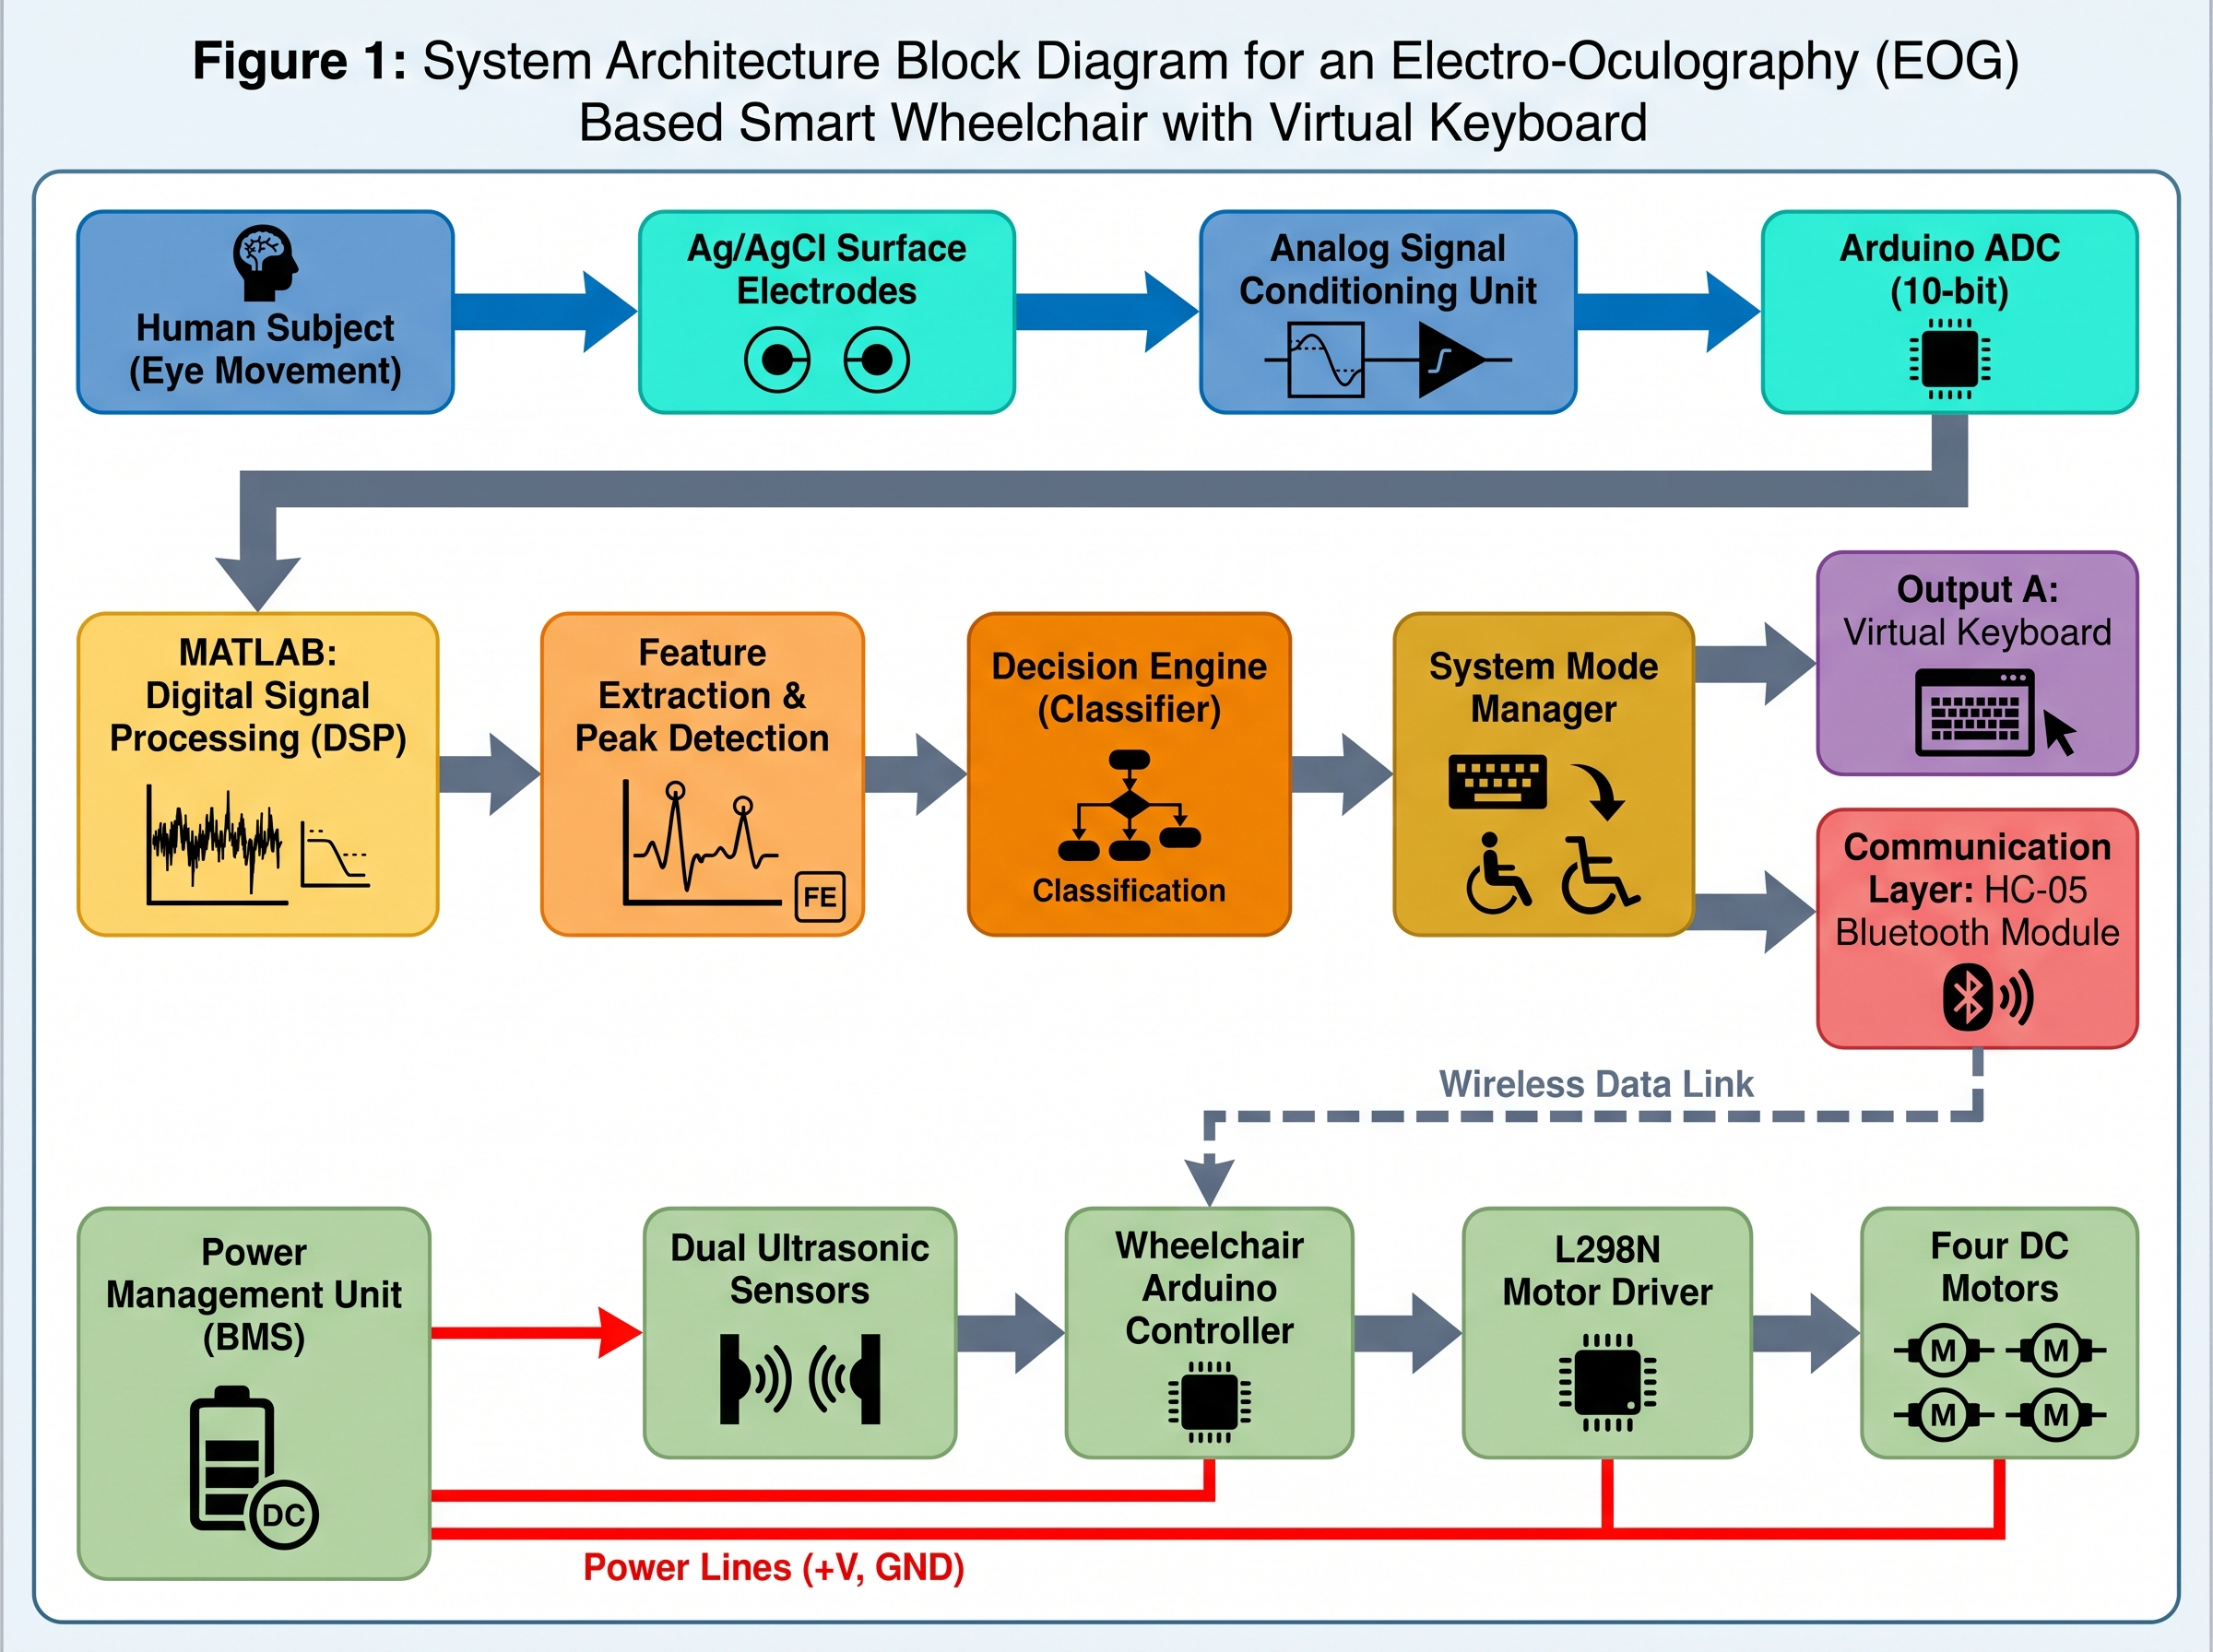
\includegraphics[width=0.82\textwidth]{system_block_diagram.jpeg}
\caption{Overall System Block Diagram illustrating the Input Stage, Processing Unit, Output Stage, and Power Management Unit.}
\label{fig:overall_block_diagram}
\end{figure}

\begin{enumerate}[label=\textbf{\arabic*.}]
    \item \textbf{Input Stage:} Bio-potential skin electrodes, differential bio-amplifier, active analog filters, and DC level conditioning.
    \item \textbf{Processing Unit:} Primary signal processing unit (MATLAB environment) for blink detection and feature extraction, interconnected with a real-time embedded microcontroller unit.
    \item \textbf{Output Stage:} Dual output actuators consisting of the motorized 3D-printed prototype wheelchair drive mechanism and the Graphical User Interface (GUI) virtual speller.
    \item \textbf{Power Management Unit:} Regulated power distribution network supplying dual symmetric voltage rails for analog signal conditioning and logic power for digital modules.
\end{enumerate}



% ============================================================
% Section 3.2: Subsystem Architecture Breakdown
% ============================================================
\section{Subsystem Architecture Breakdown}
\label{sec:subsystem_architecture_breakdown}
\label{sec:system_operations_description}

This section details the functional architecture of the four subsystems comprising the integrated EOG-guided assistive platform, detailing the signal transformation pipeline from biopotential sensing to actuation and virtual communication.

% ----------------------------------------------------------
% Subsystem 1: Biopotential Acquisition & AFE
% ----------------------------------------------------------
\subsection{Subsystem 1: Biopotential Acquisition and Analog Front-End (AFE)}
\label{subsec:subsystem1_afe}
\label{subsec:physiological_signal_generation}
\label{subsec:differential_amplification}
\label{subsec:analog_bandpass_filtering}
\label{subsec:dc_level_shifting}

\begin{itemize}
    \item \textbf{Ag/AgCl Surface Electrodes:} Detects the microvolt-level potential differences generated by the standing corneo-retinal dipole during voluntary eye movements and blinks. Electrodes are placed in a vertical periorbital configuration with a forehead reference electrode.
    \item \textbf{Instrumentation Amplifier Stage (AD620):} Provides primary differential amplification for weak raw EOG potentials ($\approx 100\,\mu\text{V} - 600\,\mu\text{V}$). The stage provides a Common-Mode Rejection Ratio ($\text{CMRR} > 100\text{ dB}$) and an input impedance of $10^{10}\,\Omega$ to reject power-line noise and prevent skin-electrode loading effects.
    \item \textbf{Active Filtering Cascade (TL072 Op-Amps):} Consists of a second-order active Sallen-Key High-Pass Filter ($f_c = 0.8\text{ Hz}$) to remove half-cell potential DC offsets and motion baseline drift, followed by a second-order Low-Pass Filter ($f_c = 30\text{ Hz}$) to eliminate high-frequency electromyographic (EMG) muscle artifacts.
    \item \textbf{50 Hz Power-Line Notch Filter:} A dedicated active notch filter sharply attenuates $50\text{ Hz}$ ambient electromagnetic hum coupled from surrounding power infrastructure.
    \item \textbf{DC Level Shifter:} Adds a stable $+2.5\text{ V}$ DC offset to the amplified bipolar signal ($\pm V$), converting it into a purely positive unipolar waveform ($0\text{ V} - 5\text{ V}$) fully compatible with the analog input limits of the microcontroller.
\end{itemize}

% ----------------------------------------------------------
% Subsystem 2: Digitization & Central DSP Pipeline
% ----------------------------------------------------------
\subsection{Subsystem 2: Digitization and Central Signal Processing Pipeline}
\label{subsec:subsystem2_dsp}
\label{subsec:sampling_quantization}
\label{subsec:serial_telemetry}
\label{subsec:serial_data_streaming}
\label{subsec:digital_signal_filtering}
\label{subsec:feature_extraction_classification}

\begin{itemize}
    \item \textbf{Analog-to-Digital Conversion (ADC):} The conditioned analog waveform is sampled by a 10-bit embedded ADC at a continuous sampling frequency ($F_s = 250\text{ Hz}$), quantizing the $0-5\text{ V}$ input into digital values ($0-1023$).
    \item \textbf{Serial Data Streaming:} Digitized biopotential samples are packaged and transmitted to the host environment via UART serial communication at a baud rate of $115200\text{ bps}$.
    \item \textbf{MATLAB DSP Engine:} Applies dynamic moving-average envelope filtering and secondary digital Butterworth notch filtering to yield a clean, smoothed waveform.
    \item \textbf{Feature Extraction \& Peak Detection:} Computes instantaneous signal amplitude against defined threshold levels ($V_{th}$) and measures the pulse time duration ($T_{width}$) to reliably discriminate intentional control blinks from involuntary spontaneous blinks.
\end{itemize}

% ----------------------------------------------------------
% Subsystem 3: System Mode Manager & Output Interfaces
% ----------------------------------------------------------
\subsection{Subsystem 3: System Mode Manager and Output Interfaces}
\label{subsec:subsystem3_mode_manager}
\label{subsec:fsm_decision_engine}
\label{subsec:system_mode_management}
\label{subsec:virtual_keyboard_gui}

\begin{itemize}
    \item \textbf{Finite State Machine (FSM) Mode Manager:} Serves as the central decision engine. It interprets blink counts and temporal sequences. Upon classifying a four-blink trigger sequence, the FSM toggles the active operational context between communication and mobility modes.
    \item \textbf{Virtual Optical Speller (Mode A):} When active, classified blink commands drive a circular 6-sector auto-scanning interface, enabling hands-free Arabic text entry, editing, and display management.
    \item \textbf{Wireless Telemetry (Mode B):} When Wheelchair Mode is active, classified directional commands are converted into control bytes and passed to an HC-05 Bluetooth master module for wireless transmission.
\end{itemize}

% ----------------------------------------------------------
% Subsystem 4: Autonomous Robotic Wheelchair & Safety Override
% ----------------------------------------------------------
\subsection{Subsystem 4: Autonomous Robotic Wheelchair and Safety Override}
\label{subsec:subsystem4_wheelchair_safety}
\label{subsec:smart_wheelchair_control}

\begin{itemize}
    \item \textbf{Embedded Control Receiver:} An HC-05 slave receiver mounted on the prototype wheelchair receives the wireless control frames and forwards them to the navigation microcontroller.
    \item \textbf{Ultrasonic Safety Array (HC-SR04):} Continuously polls front ($40\text{ cm}$ threshold) and rear ($30\text{ cm}$ threshold) distances using Time-of-Flight (ToF) acoustic measurements.
    \item \textbf{Autonomous Safety Override:} If an environmental obstacle breaches the safety perimeter, an immediate hardware interrupt suspends active user EOG drive commands, arresting motor power and triggering an automated escape rotation.
    \item \textbf{H-Bridge Power Stage \& Actuation (L298N \& DC Motors):} Drives four geared DC motors configured in a differential steering layout. The driver applies Pulse-Width Modulation (PWM) signals to ensure smooth acceleration, linear speed regulation, and zero-radius turns.
\end{itemize}

% ============================================================
% Section 3.3: System Flowcharts
% ============================================================
\section{System Flowcharts}
\label{sec:system_flowcharts}

System software behavior is governed by the master system operation flowchart illustrated in Figure~\ref{fig:master_system_flowchart}, alongside three primary sub-flowcharts executing concurrently across the host processing unit and embedded microcontroller.

\begin{figure}[H]
  \centering
  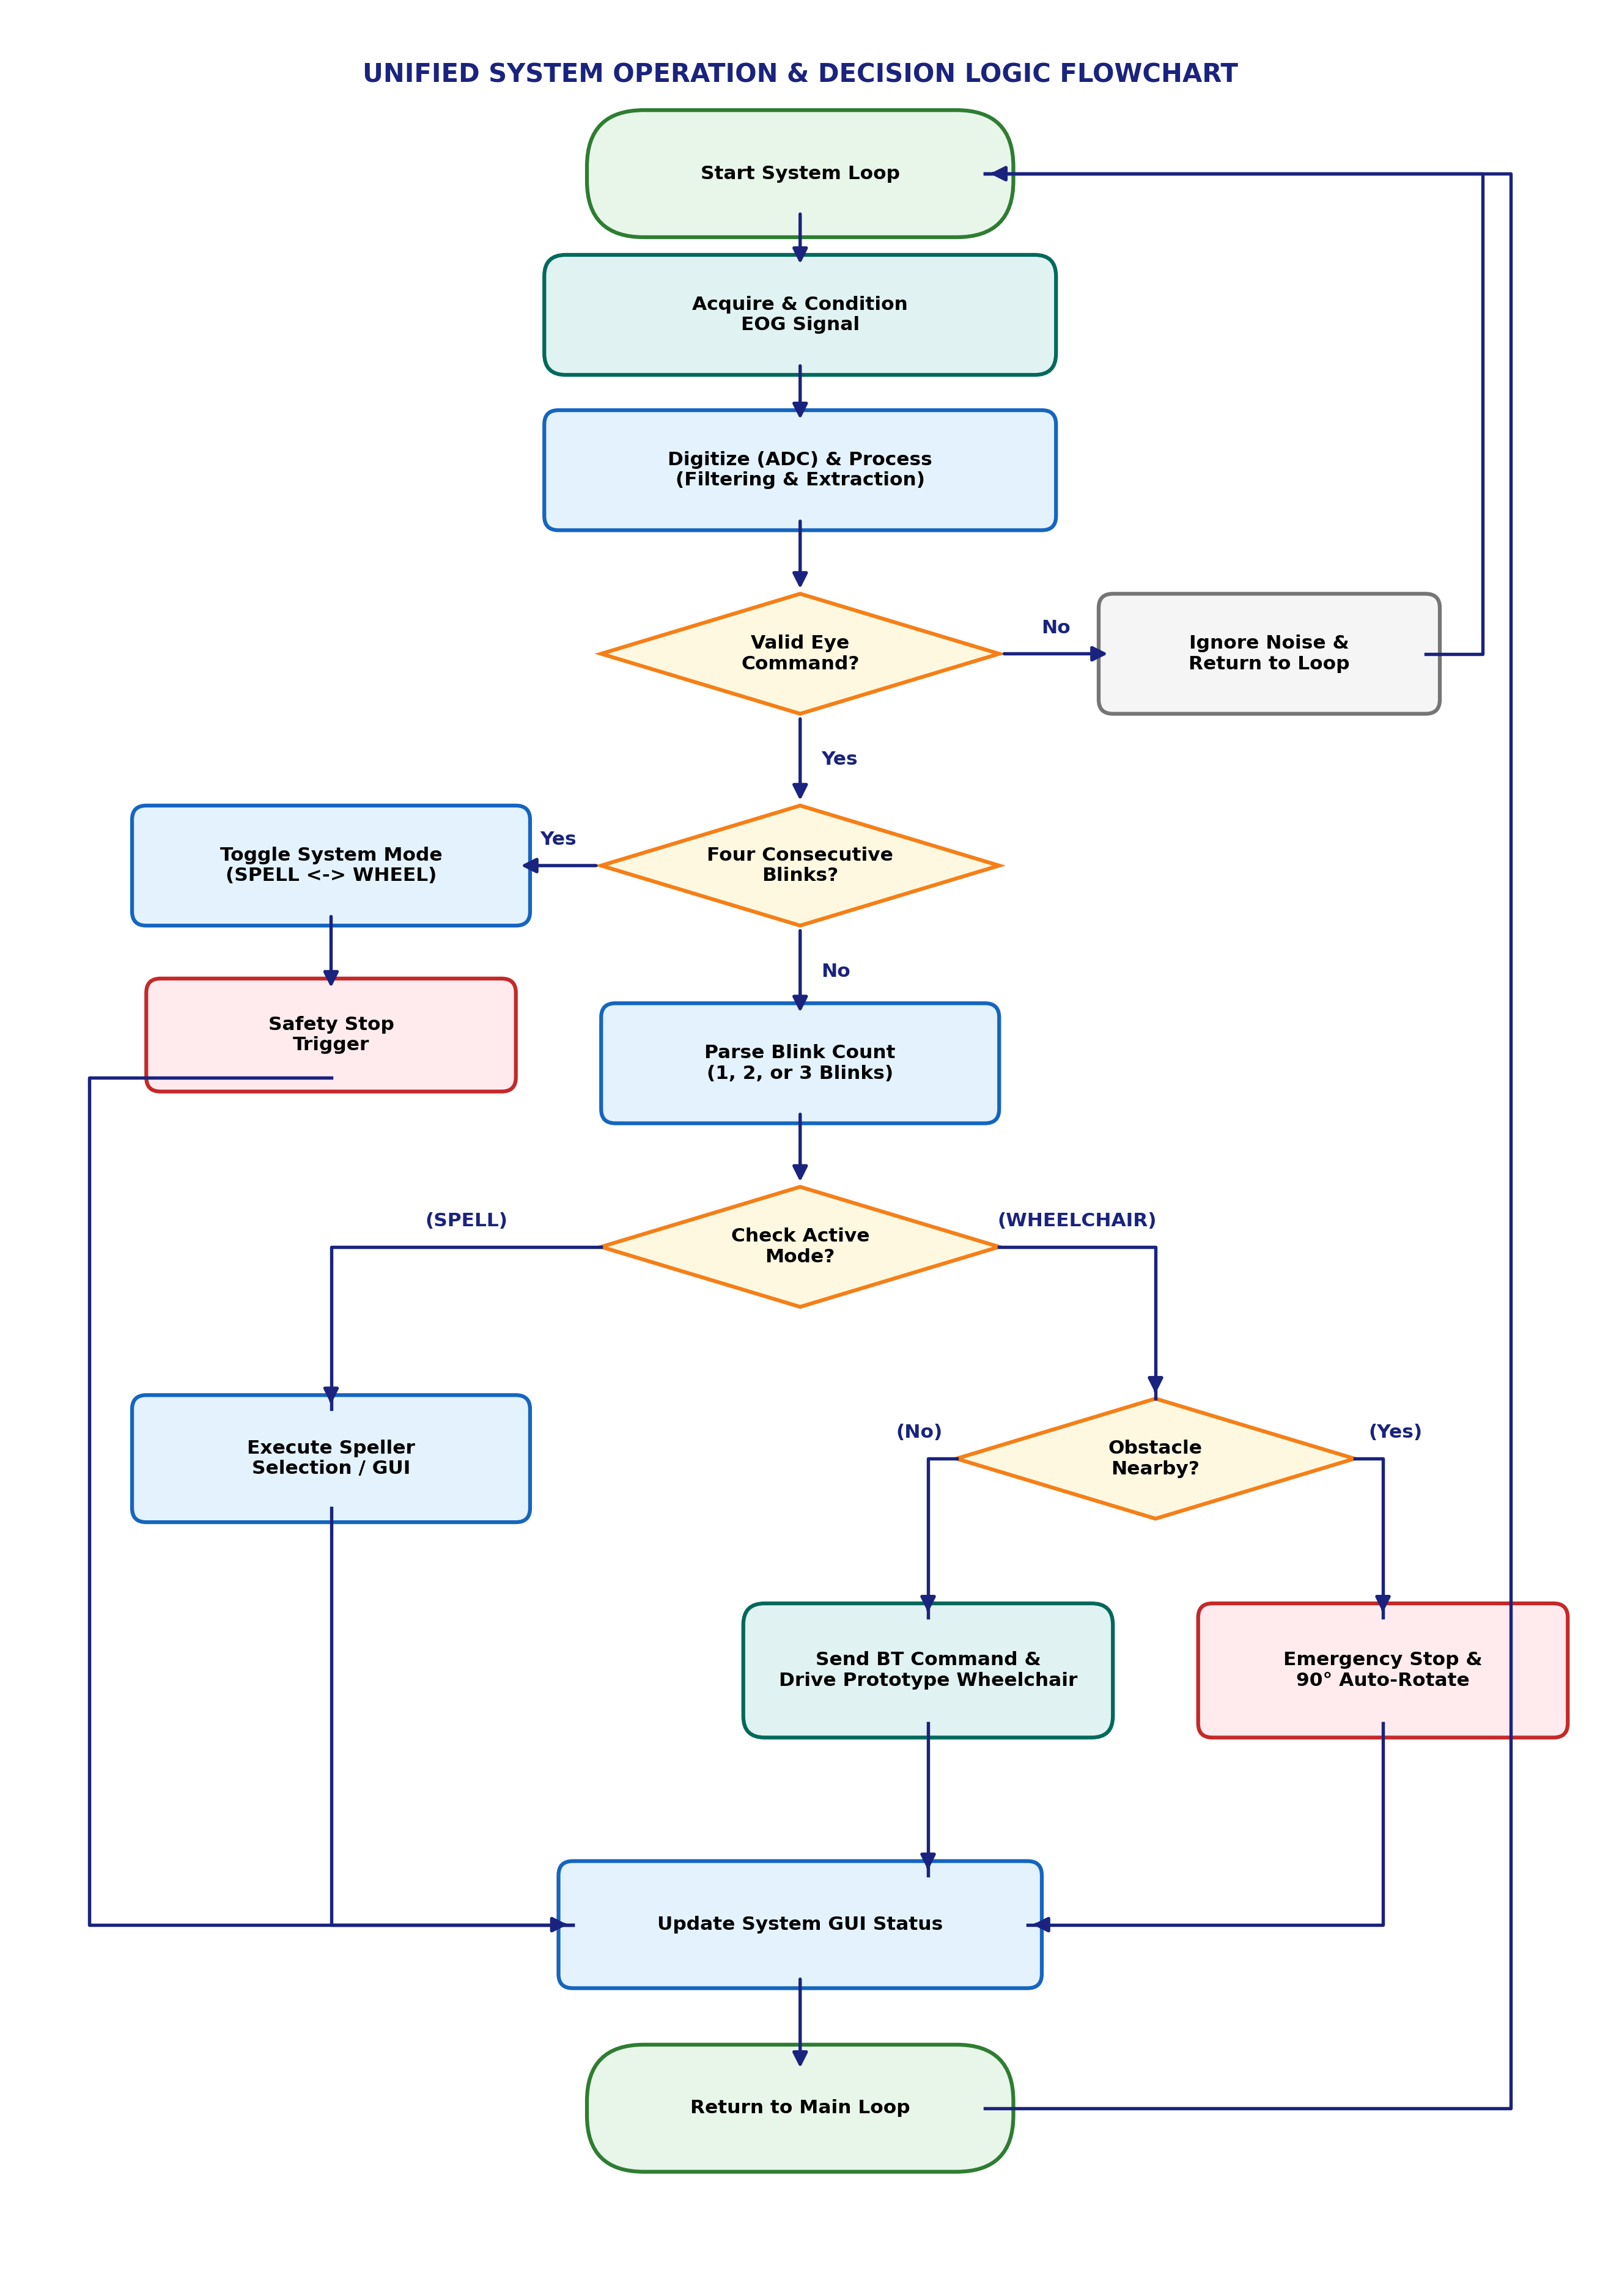
\includegraphics[width=0.88\textwidth]{master_system_flowchart.png}
  \caption{Unified System Operation and Decision Logic Flowchart.}
  \label{fig:master_system_flowchart}
\end{figure}

\FloatBarrier
\subsection{EOG Signal Acquisition, Processing, and Validation (MATLAB)}
\label{subsec:flowchart_matlab}

The master execution loop initiates with the continuous acquisition of ocular micro-biopotentials via surface Ag/AgCl electrodes (\textit{Start System Loop}). The raw physiological signal undergoes primary analog conditioning---utilizing the AD620 instrumentation amplifier and TL072 active filters---before being digitized by the microcontroller's ADC at a locked frequency of $250\,\text{Hz}$ (\textit{Acquire \& Condition EOG Signal}).

Upon transmission to the MATLAB environment, the digital signal is refined using a $50\,\text{Hz}$ Notch filter and a moving-average algorithm to eliminate power-line hum and baseline noise (\textit{Digitize \& Process}). Subsequently, the algorithm evaluates the waveform against predefined amplitude thresholds (\textit{Valid Eye Command?}). If the signal fails to meet the strict criteria (e.g., spontaneous blinks or motion artifacts), the system classifies it as a false trigger, ignoring the noise and resetting the cycle (\textit{Ignore Noise \& Return to Loop}). Only valid, intentional blink transients are permitted to proceed to the classification engine.

\FloatBarrier
\subsection{Unified System Mode Switching and Routing Logic}
\label{subsec:flowchart_mode_switching}

Once an intentional ocular command is validated, the Decision Engine determines the system's operational path based on the temporal blink sequence. The logic first evaluates whether a high-level toggle sequence has been executed (\textit{Four Consecutive Blinks?}).

If exactly four blinks are detected (\textit{Yes}), the system executes a mode transition (\textit{Toggle System Mode: SPELL $\leftrightarrow$ WHEEL}). Crucially, to ensure patient safety during this macro-state transition, a \textit{Safety Stop Trigger} is simultaneously activated, automatically placing the wheelchair into a STANDBY state to prevent sudden, uncommanded physical movement.

If the sequence contains fewer than four blinks (\textit{No}), the logic progresses to evaluate the specific gesture (\textit{Parse Blink Count: 1, 2, or 3 Blinks}) and routes the command based on the currently active macro-state (\textit{Check Active Mode?}):

\begin{itemize}
    \item \textbf{Virtual Speller Mode (SPELL):} The system routes the command to the GUI (\textit{Execute Speller Selection}). The parsed blink count dictates the typing action: 1 blink executes sector/character selection, 2 blinks trigger a space or single-character backspace, and 3 blinks clear the text display.

    \item \textbf{Wheelchair Mode (WHEELCHAIR):} The parsed directional command is routed to the physical navigation and safety layer.
\end{itemize}

\FloatBarrier
\subsection{Autonomous Obstacle Avoidance and Output Actuation Flowchart}
\label{subsec:flowchart_arduino}

When operating in Wheelchair Mode, user commands are not executed blindly. Before any directional command is translated into physical actuation, the decision logic queries the embedded ultrasonic safety layer (\textit{Obstacle Nearby?}).

\begin{itemize}
    \item \textbf{Collision Imminent (Yes):} If an environmental obstacle breaches the strict proximity thresholds, the user's directional intent is immediately overridden. The system executes a hardware-level intervention (\textit{Emergency Stop \& $90^\circ$ Auto-Rotate}), autonomously halting the vehicle and rotating it until a clear path is verified.

    \item \textbf{Clear Path (No):} If the safety perimeters are clear, the validated movement command is encoded and transmitted via the wireless serial link to the motor driver (\textit{Send BT Command \& Drive Prototype Wheelchair}).
\end{itemize}

Ultimately, both the spelling and navigation execution branches converge at a final visualization block (\textit{Update System GUI Status}). This ensures the user receives real-time visual feedback on the host display---reflecting typed characters, active wheelchair directions, or standby states. The cycle then concludes (\textit{Return to Main Loop}), resetting the buffers to acquire the next biopotential command.



% --- Chapter Conclusion & Transition ---
\vspace{1em}
To summarize, this chapter established the high-level architectural framework, mode switching logic, and operational flowcharts governing wheelchair navigation and virtual speller control. Having finalized the abstract functional workflow, Chapter 4 transitions to physical hardware realization, detailing circuit simulations, IC specifications (AD620, L298N), mathematical design calculations, and the hybrid software implementation.


% Chapter 4: Circuit Simulation & Implementation
% ============================================================
% Chapter 4: Circuit Simulation and Hardware Implementation
% ============================================================
\chapter{Circuit Simulation and Hardware Implementation}
\label{ch:implementation}

\chapteroverview{This chapter details the physical hardware component specifications, analog circuit simulations, mathematical calculations, breadboard prototyping, embedded safety systems, 3D-printed wheelchair chassis, and complete physical system integration of the EOG-guided assistive platform.}


% ============================================================
% Section 4.1: Hardware Components Specifications
% ============================================================
\section{Hardware Components Specifications}
\label{sec:hardware_components_specifications}

To realize the integrated assistive platform, specific off-the-shelf electronic modules, power management systems, and integrated circuits were carefully selected based on their precision, power efficiency, and compatibility. Below is a technical breakdown of the primary hardware components utilized in both the analog front-end and the embedded control layers.

\FloatBarrier
\subsection{Instrumentation Amplifier (AD620)}
\label{ad620_spec}

\noindent\textbf{Technical Specs:} The AD620 is a high-accuracy instrumentation amplifier that requires only one external resistor to set gains from 1 to 10,000. It features a high Common-Mode Rejection Ratio ($\text{CMRR} > 100\,\text{dB}$), a low maximum offset voltage of $50\,\mu\text{V}$, and a low input bias current of $1.0\,\text{nA}$.

\noindent\textbf{Design Justification:} This IC was chosen as the primary pre-amplifier (Stage 1) because its high input impedance ($10^{10}\,\Omega$) prevents loading the skin-electrode interface. Its high CMRR effectively rejects $50\,\text{Hz}$ power-line hum picked up by the human body during EOG acquisition.

\begin{figure}[H]
\centering
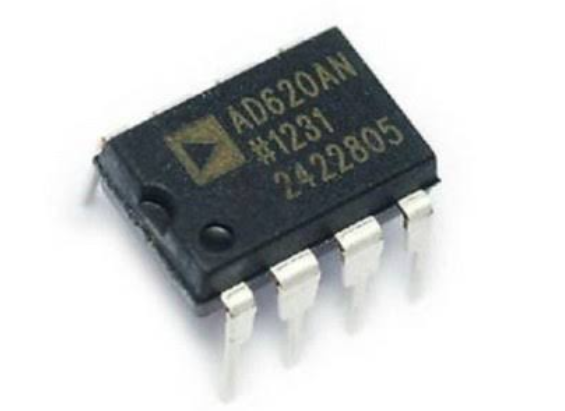
\includegraphics[width=0.45\textwidth]{ad620_ic.png}
\caption{AD620 Instrumentation Amplifier IC.}
\label{fig:ad620_ic_photo}
\end{figure}

\FloatBarrier
\subsection{Dual Operational Amplifier (TL072)}
\label{tl072_spec}

\noindent\textbf{Technical Specs:} The TL072 is a high-speed JFET-input dual operational amplifier providing low noise ($18\,\text{nV}/\sqrt{\text{Hz}}$), minimal power consumption, and a high slew rate ($13\,\text{V}/\mu\text{s}$).

\noindent\textbf{Design Justification:} Two TL072 ICs were utilized to construct the active Sallen-Key filters (High-pass and Low-pass), the $50\,\text{Hz}$ notch filter, and the DC level shifter. The JFET inputs ensure minimal signal distortion and preserve the integrity of the microvolt-level EOG transients.

\begin{figure}[H]
\centering
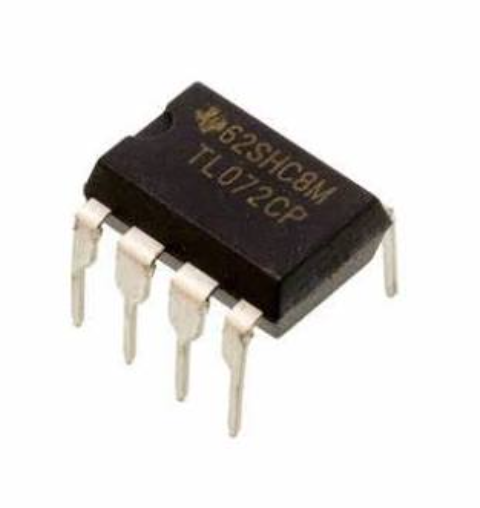
\includegraphics[width=0.45\textwidth]{tl072_ic.png}
\caption{TL072 JFET-Input Dual Operational Amplifier.}
\label{fig:tl072_ic_photo}
\end{figure}

\FloatBarrier
\subsection{Bluetooth SPP Module (HC-05)}
\label{hc05_spec}

\noindent\textbf{Technical Specs:} The HC-05 operates on the $2.4\,\text{GHz}$ ISM band using Bluetooth V2.0+EDR and supports variable UART baud rates up to $115,200\,\text{bps}$.

\noindent\textbf{Design Justification:} It was selected to establish a reliable, zero-latency wireless telemetry link between the MATLAB host environment and the wheelchair’s embedded microcontroller, ensuring complete physical isolation and independent mobility for the user.

\begin{figure}[H]
\centering
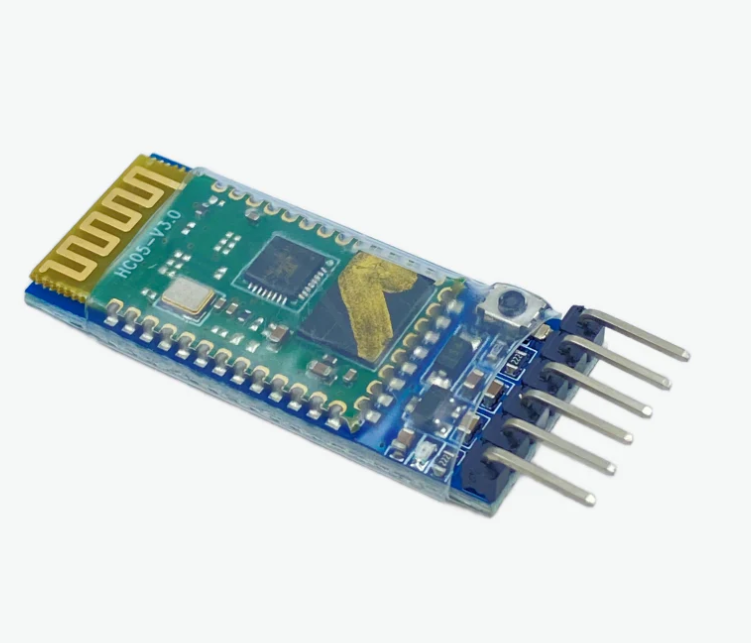
\includegraphics[width=0.45\textwidth]{hc05_bluetooth.png}
\caption{HC-05 Bluetooth Module for wireless telemetry.}
\label{fig:hc05_bluetooth_photo}
\end{figure}

\FloatBarrier
\subsection{Dual H-Bridge Motor Driver (L298N)}
\label{l298n_spec}

\noindent\textbf{Technical Specs:} The L298N is a high-voltage, high-current dual full-bridge driver designed to accept standard TTL logic levels and drive inductive loads up to $2\,\text{A}$ per channel.

\noindent\textbf{Design Justification:} This module efficiently translates the low-current Pulse-Width Modulation (PWM) signals from the Arduino into the high-current power required by the DC motors, enabling precise speed regulation and bidirectional rotation for the wheelchair chassis.

\begin{figure}[H]
\centering
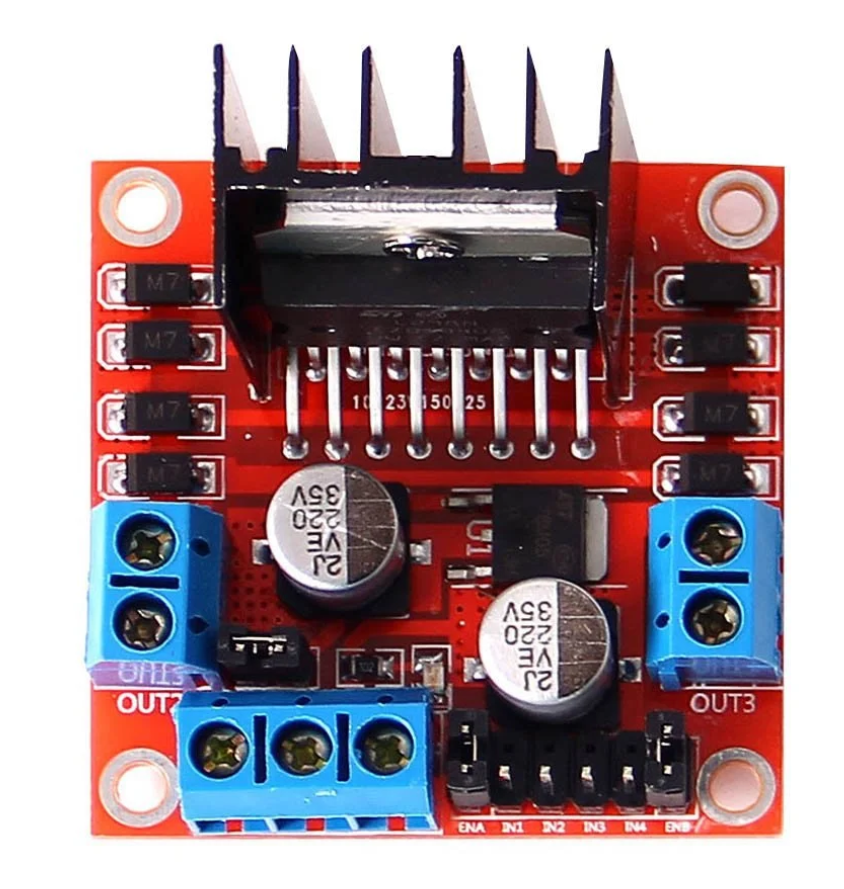
\includegraphics[width=0.45\textwidth]{l298n_driver.png}
\caption{L298N Dual H-Bridge Motor Driver.}
\label{fig:l298n_driver_photo}
\end{figure}

\FloatBarrier
\subsection{Geared DC Motors (TT Motors)}
\label{tt_motor_spec}

\noindent\textbf{Technical Specs:} The TT DC gear motors operate optimally between $3\,\text{V}$ and $6\,\text{V}$, featuring an internal gear reduction ratio of $1:48$ to maximize torque at lower rotational speeds.

\noindent\textbf{Design Justification:} Four TT motors were selected for the 4-Wheel Drive (4WD) configuration. Their balanced torque-to-speed ratio enables the 3D-printed chassis to perform smooth acceleration, overcome floor friction, and execute full 360-degree zero-radius turns without drawing excessive current.

\begin{figure}[H]
\centering
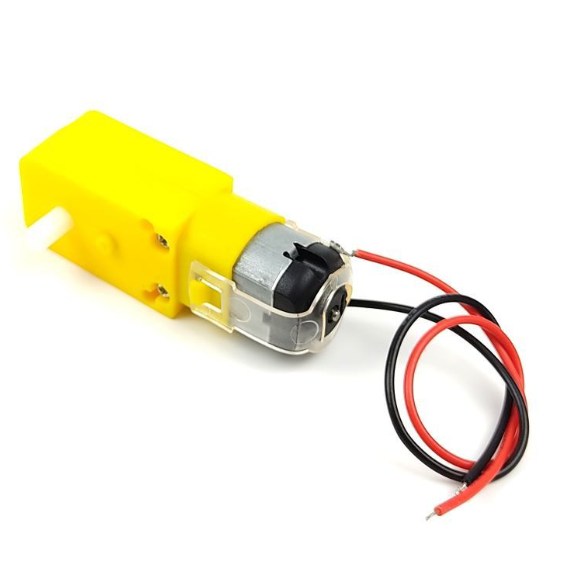
\includegraphics[width=0.45\textwidth]{tt_motor.png}
\caption{TT Geared DC Motor ($1:48$ Ratio).}
\label{fig:tt_motor_photo}
\end{figure}

\FloatBarrier
\subsection{Ultrasonic Time-of-Flight Sensor (HC-SR04)}
\label{hcsr04_spec}

\noindent\textbf{Technical Specs:} The HC-SR04 provides non-contact distance measurement from $2\,\text{cm}$ to $400\,\text{cm}$ with an acoustic ranging accuracy of up to $3\,\text{mm}$.

\noindent\textbf{Design Justification:} Two sensors were integrated into the front and rear of the wheelchair. They continuously poll environmental proximity independently of the EOG inputs to trigger autonomous emergency stops, forming the core of the localized safety override layer.

\begin{figure}[H]
\centering
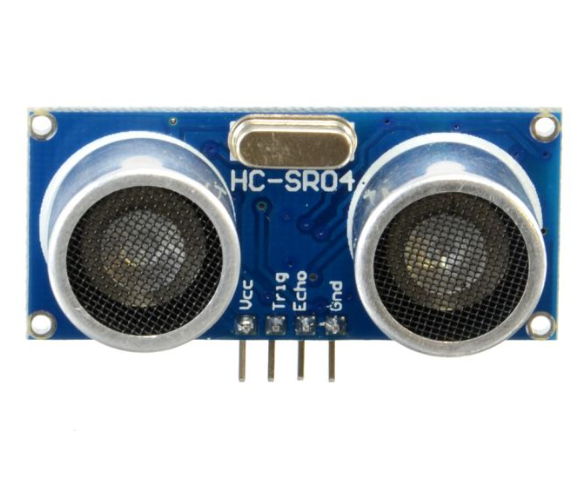
\includegraphics[width=0.45\textwidth]{hcsr04_sensor.png}
\caption{HC-SR04 Ultrasonic Distance Sensor.}
\label{fig:hcsr04_sensor_photo}
\end{figure}

\FloatBarrier
\subsection{Power Supply System: Lithium-Ion Cells and BMS}
\label{power_system_spec}

\noindent\textbf{Technical Specs:} The power bank utilizes high-capacity $3.7\,\text{V}$ Lithium-Ion cylindrical cells ($18650$ format, $1200\,\text{mAh}$) managed by a 3S $40\,\text{A}$ Battery Management System (BMS) protection board.

\noindent\textbf{Design Justification:} To prevent electromagnetic interference from motor switching noise, the system employs isolated power distribution. The Li-ion cells provide high energy density for prolonged operation, while the 3S $40\,\text{A}$ BMS ensures cell balancing, overcharge protection, and safe current delivery during peak motor loads.

\begin{figure}[H]
\centering
\begin{subfigure}[b]{0.48\textwidth}
    \centering
    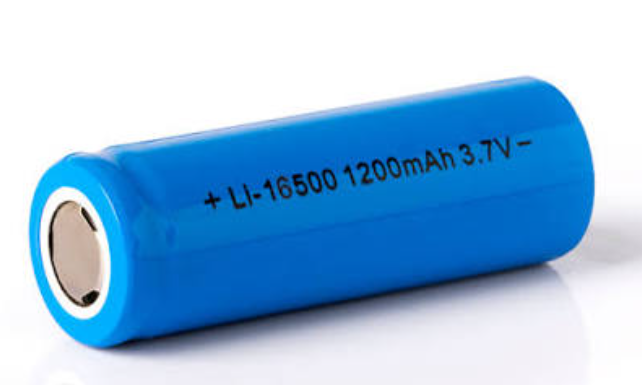
\includegraphics[width=\textwidth]{liion_cell.png}
    \caption{3.7V Lithium-Ion 18650 Cell.}
    \label{fig:liion_cell_photo}
\end{subfigure}
\hfill
\begin{subfigure}[b]{0.48\textwidth}
    \centering
    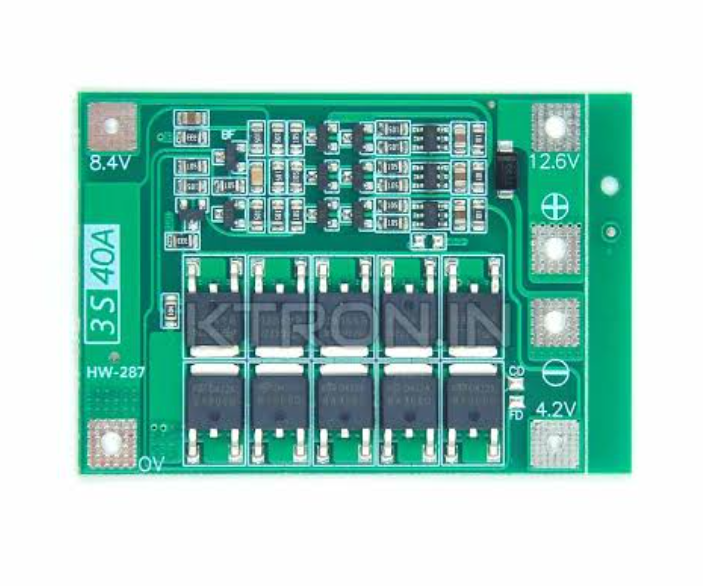
\includegraphics[width=\textwidth]{bms_board.png}
    \caption{3S 40A Battery Management System (BMS) Board.}
    \label{fig:bms_board_photo}
\end{subfigure}
\caption{Power supply system components comprising 18650 Li-ion cells and 3S 40A BMS protection board.}
\label{fig:power_supply_system_components}
\end{figure}

% ============================================================
% Section 4.2: Analog Circuit Simulation and Mathematical Derivations
% ============================================================
\section{Analog Circuit Simulation and Mathematical Derivations}
\label{sec:circuit_simulation_math_derivations}

Prior to physical prototype assembly, the complete multi-stage analog signal conditioning cascade was modeled and simulated using Proteus VSM and SPICE simulation tools to verify stability, gain linearity, active filter frequency response, and power line noise rejection characteristics. Figure \ref{fig:eog_circuit_schematic} illustrates the complete hardware schematic diagram of the EOG bio-potential conditioning circuit.

\begin{figure}[H]
  \centering
  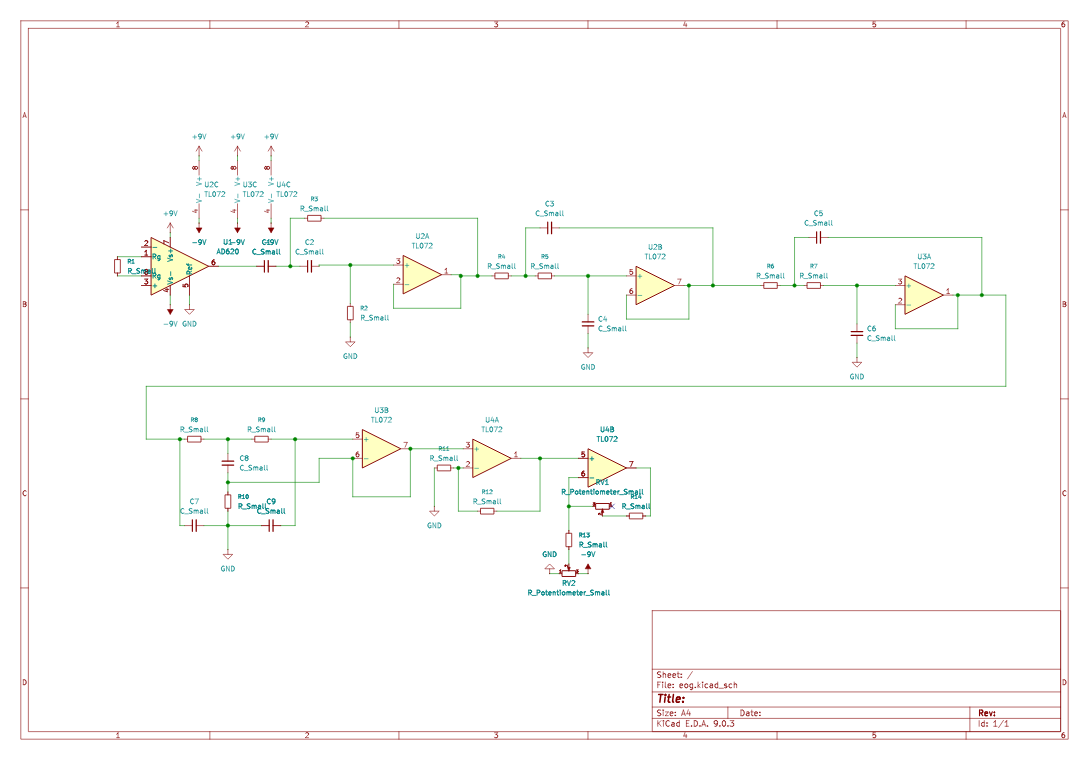
\includegraphics[width=1.0\textwidth]{eog_circuit.png}
  \caption{Complete schematic diagram of the multi-stage EOG analog front-end circuit.}
  \label{fig:eog_circuit_schematic}
\end{figure}

\FloatBarrier
\subsection{Bipolar Power Supply Management}
\label{subsec:bipolar_power_supply}

Biopotential signals such as Electrooculography (EOG) exhibit alternating current (AC) characteristics around a zero-volt baseline with microvolt-level amplitudes. To process these signals without symmetrical waveform distortion, dynamic range degradation, or peak clipping, the analog signal conditioning subsystem requires a symmetric dual-polarity power supply configuration ($\pm 9\,\text{V}$).

The system utilizes independent DC power sources to decouple power line noise from the sensitive analog front-end. The voltage rails are configured as follows:
\begin{itemize}
    \item \textbf{$V_{\text{CC}} = +9\,\text{V}$:} Connected to the positive supply pins of the instrumentation and operational amplifiers.
    \item \textbf{$V_{\text{EE}} = -9\,\text{V}$:} Connected to the negative supply pins.
    \item \textbf{$\text{GND} = 0\,\text{V}$:} Serves as the system analog reference ground point.
\end{itemize}

\FloatBarrier
\subsection{Multi-Stage Hardware Topology}
\label{subsec:multistage_hardware_topology}

The physical signal conditioning circuit consists of four integrated circuits (ICs)---one AD620 Instrumentation Amplifier and three TL072 Low-Noise JFET-Input Dual Operational Amplifiers---divided into four sequential processing stages. Figure \ref{fig:afe_processing_cascade} illustrates the functional processing sequence from electrode acquisition to microcontroller ADC conversion.

\begin{figure}[H]
  \centering
  \resizebox{\textwidth}{!}{%
  \begin{tikzpicture}[
    node distance=0.8cm and 0.6cm,
    block/.style={
      rectangle,
      draw=navyblue,
      fill=blue!8!white,
      thick,
      rounded corners=4pt,
      minimum height=1.3cm,
      minimum width=2.8cm,
      align=center,
      font=\sffamily\small
    },
    sensor/.style={
      rectangle,
      draw=darkgreen,
      fill=green!10!white,
      thick,
      rounded corners=4pt,
      minimum height=1.3cm,
      minimum width=2.5cm,
      align=center,
      font=\sffamily\small
    },
    mcu/.style={
      rectangle,
      draw=darkred,
      fill=red!10!white,
      thick,
      rounded corners=4pt,
      minimum height=1.3cm,
      minimum width=2.5cm,
      align=center,
      font=\sffamily\small
    },
    arrow/.style={
      ->,
      >=Stealth,
      thick,
      line width=1.2pt,
      draw=navyblue
    }
  ]

    % Row 1 (Left to Right)
    \node (electrodes) [sensor] {\textbf{Ag/AgCl Electrodes}\\[-2pt]\tiny (Periorbital Sensors)};
    \node (stage1) [block, right=of electrodes] {\textbf{Stage 1: AD620}\\[-2pt]\tiny (Pre-Amp, $G_1 \approx 6\times$)};
    \node (stage2) [block, right=of stage1] {\textbf{Stage 2: HPF \& LPF}\\[-2pt]\tiny (Active $0.8\text{ Hz} - 30\text{ Hz}$)};
    \node (stage3) [block, right=of stage2] {\textbf{Stage 3: Notch \& $G_2$}\\[-2pt]\tiny ($50\text{ Hz}$ Notch, $G_2 = 10\times$)};

    % Row 2 (Right to Left)
    \node (stage4a) [block, below=1.2cm of stage3] {\textbf{Stage 4: Variable Gain}\\[-2pt]\tiny ($G_3 = 10\times - 100\times$)};
    \node (stage4b) [block, left=of stage4a] {\textbf{Stage 4: Level Shifter}\\[-2pt]\tiny (DC Offset $+2.5\text{ V}$)};
    \node (arduino) [mcu, left=of stage4b] {\textbf{Arduino Uno ADC}\\[-2pt]\tiny ($0\text{ V} - 5\text{ V}$ 10-bit Input)};

    % Connections
    \draw [arrow] (electrodes) -- (stage1);
    \draw [arrow] (stage1) -- (stage2);
    \draw [arrow] (stage2) -- (stage3);
    \draw [arrow] (stage3.south) -- (stage4a.north);
    \draw [arrow] (stage4a) -- (stage4b);
    \draw [arrow] (stage4b) -- (arduino);

  \end{tikzpicture}%
  }
  \caption{Sequential multi-stage processing cascade of the EOG analog front-end.}
  \label{fig:afe_processing_cascade}
\end{figure}

\FloatBarrier
\subsection{Mathematical Derivations \& Theoretical Circuit Calculations}
\label{subsec:mathematical_derivations_calculations}

Rigorous analytical design ensures that voltage gains, filter corner frequencies, and system dynamic ranges meet biomedical operational design specifications.

\FloatBarrier
\subsubsection{Stage 1 Gain Calculation (AD620)}
\label{subsubsec:stage1_gain_calc}

The differential voltage gain ($G_1$) of the AD620 instrumentation amplifier is defined by:
\begin{equation}
G_1 = 1 + \frac{49.4\,\text{k}\Omega}{R_G}
\label{eq:ad620_gain_formula}
\end{equation}

Given a gain-setting resistor $R_G = 10\,\text{k}\Omega$:
\begin{equation}
G_1 = 1 + \frac{49.4\,\text{k}\Omega}{10\,\text{k}\Omega} = 1 + 4.94 = 5.94 \approx 6\times
\label{eq:ad620_gain_result}
\end{equation}

\FloatBarrier
\subsubsection{\texorpdfstring{High-Pass Filter Cutoff Frequency ($f_{c,\text{HPF}}$)}{High-Pass Filter Cutoff Frequency (fc,HPF)}}
\label{subsubsec:hpf_cutoff_calc}

The corner frequency ($f_{c,\text{HPF}}$) of the active Sallen-Key high-pass filter is determined by:
\begin{equation}
f_{c,\text{HPF}} = \frac{1}{2\pi \cdot R_{\text{HPF}} \cdot C_{\text{HPF}}}
\label{eq:hpf_formula}
\end{equation}

Given $R_{\text{HPF}} = 200\,\text{k}\Omega = 200 \times 10^3\,\Omega$ and $C_{\text{HPF}} = 0.9\,\mu\text{F} = 0.9 \times 10^{-6}\,\text{F}$:
\begin{equation}
f_{c,\text{HPF}} = \frac{1}{2\pi \times (200 \times 10^3) \times (0.9 \times 10^{-6})} = \frac{1}{1.13097} \approx 0.884\,\text{Hz} \approx 0.8\,\text{Hz}
\label{eq:hpf_result}
\end{equation}

\FloatBarrier
\subsubsection{\texorpdfstring{Low-Pass Filter Cutoff Frequency ($f_{c,\text{LPF}}$)}{Low-Pass Filter Cutoff Frequency (fc,LPF)}}
\label{subsubsec:lpf_cutoff_calc}

The corner frequency ($f_{c,\text{LPF}}$) of the active Sallen-Key low-pass filter is given by:
\begin{equation}
f_{c,\text{LPF}} = \frac{1}{2\pi \cdot R_{\text{LPF}} \cdot C_{\text{LPF}}}
\label{eq:lpf_formula}
\end{equation}

Given $R_{\text{LPF}} = 27\,\text{k}\Omega = 27 \times 10^3\,\Omega$ and $C_{\text{LPF}} = 0.2\,\mu\text{F} = 0.2 \times 10^{-6}\,\text{F}$:
\begin{equation}
f_{c,\text{LPF}} = \frac{1}{2\pi \times (27 \times 10^3) \times (0.2 \times 10^{-6})} = \frac{1}{0.033929} \approx 29.47\,\text{Hz} \approx 30\,\text{Hz}
\label{eq:lpf_result}
\end{equation}

\FloatBarrier
\subsubsection{\texorpdfstring{Notch Filter Rejection Frequency ($f_{\text{notch}}$)}{Notch Filter Rejection Frequency (fnotch)}}
\label{subsubsec:notch_cutoff_calc}

The notch rejection frequency ($f_{\text{notch}}$) for power-line noise reduction is given by:
\begin{equation}
f_{\text{notch}} = \frac{1}{2\pi \cdot R_{\text{notch}} \cdot C_{\text{notch}}}
\label{eq:notch_formula}
\end{equation}

With $C_{\text{notch}} = 0.2\,\mu\text{F}$ and the variable potentiometer calibrated to $R_{\text{notch}} \approx 15.915\,\text{k}\Omega$:
\begin{equation}
f_{\text{notch}} = \frac{1}{2\pi \times (15.915 \times 10^3) \times (0.2 \times 10^{-6})} \approx 50.0\,\text{Hz}
\label{eq:notch_result}
\end{equation}

\FloatBarrier
\subsubsection{\texorpdfstring{Secondary Stage Voltage Gain ($G_2$)}{Secondary Stage Voltage Gain (G2)}}
\label{subsubsec:secondary_gain_calc}

The non-inverting operational amplifier gain ($G_2$) is expressed as:
\begin{equation}
G_2 = 1 + \frac{R_f}{R_{\text{in}}}
\label{eq:g2_formula}
\end{equation}

Given $R_f = 1\,\text{M}\Omega = 1000\,\text{k}\Omega$ and $R_{\text{in}} = 100\,\text{k}\Omega$ (scaled to yield an exact factor of $10\times$):
\begin{equation}
G_2 = 1 + \frac{1000\,\text{k}\Omega}{100\,\text{k}\Omega} = 1 + 9 = 10\times
\label{eq:g2_result}
\end{equation}

\FloatBarrier
\subsubsection{\texorpdfstring{Total System Gain Range ($A_{\text{total}}$)}{Total System Gain Range (Atotal)}}
\label{subsubsec:total_gain_calc}

The overall analog amplification factor ($A_{\text{total}}$) is the product of the cascaded individual stage gains:
\begin{equation}
A_{\text{total}} = G_1 \cdot G_2 \cdot G_3
\label{eq:atotal_formula}
\end{equation}

\begin{itemize}
    \item \textbf{Minimum Gain Bound ($G_{3,\text{min}} = 10\times$):}
    \begin{equation}
    A_{\text{total,min}} = 6 \times 10 \times 10 = 600\times
    \label{eq:atotal_min}
    \end{equation}
    \item \textbf{Maximum Gain Bound ($G_{3,\text{max}} = 100\times$):}
    \begin{equation}
    A_{\text{total,max}} = 6 \times 10 \times 100 = 6000\times
    \label{eq:atotal_max}
    \end{equation}
\end{itemize}

\begin{tcolorbox}[colback=blue!5!white,colframe=blue!75!black,title=\textbf{Biomedical Signal Conditioning Summary}]
This total dynamic system gain ($600\times - 6000\times$) reliably elevates raw microvolt EOG biopotentials ($\approx 100\,\mu\text{V} - 600\,\mu\text{V}$) into measurable voltage levels ($0.6\,\text{V} - 3.6\,\text{V}$ centered around a $+2.5\,\text{V}$ DC baseline), perfectly aligning with the dynamic input span of the Arduino 10-bit ADC ($0\,\text{V} - 5\,\text{V}$).
\end{tcolorbox}

% ============================================================
% Section 4.3: Analog Front-End Realization and Rapid Prototyping
% ============================================================
\section{Analog Front-End Realization and Rapid Prototyping}
\label{sec:afe_rapid_prototyping}

The physical implementation of the analog signal conditioning cascade was executed utilizing a modular rapid-prototyping approach on a breadboard, rather than a fixed Printed Circuit Board (PCB). This engineering decision was deliberate and necessary for clinical testing. EOG biopotentials and skin-electrode impedances vary significantly among different human subjects, requiring continuous dynamic calibration of the circuit.

The breadboard architecture facilitated real-time tuning of the variable potentiometers to adjust the differential gain ($G_3$) and the DC offset levels, ensuring that the analog-to-digital converter (ADC) never saturated regardless of the specific patient's baseline resting potential. Furthermore, it allowed manual fine-tuning of the 50\,Hz active notch filter during live testing to maximize common-mode noise rejection.

\begin{figure}[H]
\centering
\includegraphics[width=0.75\textwidth]{WhatsApp Image 2026-07-29 at 7.54.46 PM (1).jpeg}
\caption{The physical realization of the EOG analog front-end on a breadboard. This modular rapid-prototyping setup was specifically adopted to allow real-time calibration of the potentiometers and dynamic adjustment of filter stages during clinical testing.}
\label{fig:breadboard_afe_realization}
\end{figure}

% ============================================================
% Section 4.4: Embedded Control and Autonomous Safety Hardware
% ============================================================
\section{Embedded Control and Autonomous Safety Hardware}
\label{sec:embedded_control_safety_hardware}

To isolate the high-current physical actuation from the sensitive biopotential acquisition circuit, an independent embedded control layer was established. The prototype wheelchair is governed by an Arduino microcontroller interfaced with an L298N dual H-bridge motor driver.

A critical safety feature of this embedded layer is the autonomous collision avoidance system, achieved using front and rear HC-SR04 ultrasonic Time-of-Flight (ToF) sensors. The safety proximity thresholds were mathematically justified based on the system's total latency and physical inertia.

The front threshold was strictly set to $40\,\text{cm}$. Given that the digital signal processing pipeline introduces a latency of approximately $143\,\text{ms}$, combined with the Arduino's hardware interrupt response time ($70\,\text{ms}$) and the forward mechanical inertia of the motors, $40\,\text{cm}$ ensures that the prototype comes to a complete halt before physical impact at maximum velocity. Conversely, the rear threshold was set to $30\,\text{cm}$ because the programmed reverse speed is significantly lower than the forward speed, thereby requiring a shorter braking distance.

\begin{figure}[H]
\centering
\includegraphics[width=0.75\textwidth]{WhatsApp Image 2026-07-29 at 7.54.48 PM.jpeg}
\caption{Rear view of the wheelchair prototype highlighting the rear HC-SR04 ultrasonic sensor responsible for the $30\,\text{cm}$ reverse safety braking threshold.}
\label{fig:wheelchair_rear_ultrasonic_sensor}
\end{figure}

% ============================================================
% Section 4.5: Mechanical Design, Actuation, and 3D Printed Chassis
% ============================================================
\section{Mechanical Design, Actuation, and 3D Printed Chassis}
\label{sec:mechanical_design_chassis}

The structural framework of the prototype wheelchair was designed using CAD software and manufactured utilizing 3D printing technology with Polylactic Acid (PLA) material. PLA was selected for its optimal balance of structural rigidity, low weight, and cost-effectiveness.

To prevent electromagnetic interference (EMI) and organize the hardware, the chassis features a double-deck architectural design. The lower deck houses the high-current components, including the 18650 Lithium-ion battery power bank and the motor wiring, while the upper deck isolates the logic controllers and wireless communication modules.

Physical actuation is driven by a 4-Wheel Drive (4WD) system utilizing four independent TT geared DC motors. This differential steering configuration generates sufficient combined torque to overcome the gross weight of the PLA chassis and the batteries, as well as floor friction. More importantly, the 4WD differential setup enables skid-steering, allowing the wheelchair to execute zero-radius auto-rotations ($90^\circ$ turns in place) when an obstacle is detected, maximizing maneuverability in confined indoor environments.

\begin{figure}[H]
\centering
\begin{subfigure}[b]{0.48\textwidth}
    \centering
    \includegraphics[width=\textwidth]{WhatsApp Image 2026-07-29 at 7.54.45 PM.jpeg}
    \caption{Front-angled view of the 3D-printed wheelchair prototype showcasing the dual-layer PLA chassis, front ultrasonic sensor, and 18650 Li-ion battery power bank.}
    \label{fig:wheelchair_front_chassis}
\end{subfigure}
\hfill
\begin{subfigure}[b]{0.48\textwidth}
    \centering
    \includegraphics[width=\textwidth]{WhatsApp Image 2026-07-29 at 7.54.46 PM.jpeg}
    \caption{Side profile revealing the TT geared DC motors enabling 4-wheel differential drive and zero-radius skid-steering capabilities.}
    \label{fig:wheelchair_side_motors}
\end{subfigure}
\caption{3D-printed wheelchair prototype mechanical design, double-deck PLA chassis layout, and 4WD actuation assembly.}
\label{fig:wheelchair_prototype_mechanical_assembly}
\end{figure}

% ============================================================
% Section 4.6: Complete System Integration
% ============================================================
\section{Complete System Integration}
\label{sec:system_integration_experimental_setup}

The successful integration of the aforementioned subsystems resulted in a unified, functional Human-Computer Interface (HCI). During the experimental trials, surface electrodes were applied to the user’s periorbital region. The raw biopotentials were processed by the breadboard analog front-end, monitored in real-time via a digital oscilloscope to verify noise rejection, and simultaneously digitized by the microcontroller. The MATLAB processing engine successfully decoded these signals to wirelessly drive the 3D-printed wheelchair and operate the virtual speller interface without critical latency or system failure.

\begin{figure}[H]
\centering
\includegraphics[width=0.85\textwidth]{full setup.jpeg}
\caption{Complete experimental setup demonstrating real-time EOG signal acquisition, hardware conditioning on the breadboard, MATLAB digital processing on the host machine, and signal verification via oscilloscope.}
\label{fig:complete_experimental_hci_setup}
\end{figure}


% --- Chapter Conclusion & Transition ---
\vspace{1em}
In conclusion, this chapter presented the hardware component specifications, circuit simulations, mathematical design validation, breadboard front-end realization, embedded control and safety systems, 3D-printed wheelchair chassis design, and complete system integration. With the hardware physical platform fully operational, Chapter 5 presents the quantitative experimental testing results, waveform analyses, obstacle avoidance evaluations, and statistical accuracy metrics.


% Chapter 5: Results & Discussion
% ============================================================
% Chapter 5: Results and Discussion
% ============================================================
\chapter{Results and Discussion}
\label{ch:results}

\chapteroverview{This chapter presents the experimental validation and quantitative performance analysis of the integrated EOG-guided wheelchair and virtual speller platform. It evaluates raw vs. filtered EOG biopotential waveforms, DC offset cancellation, 4-blink threshold mode switching performance, autonomous obstacle avoidance response times, and virtual speller typing efficacy. Finally, it provides photographic documentation of the complete physical prototype and analyzes statistical command execution accuracy across 1000 test trials and cited Scopus literature.}


% ============================================================
% Section 5.1: EOG Signal Acquisition and Processing Results
% ============================================================
\section{EOG Signal Acquisition and Processing Results}
\label{sec:results_eog_signal}

\subsection{Subject Demographics and Testing Protocol}
\label{subsec:subject_demographics_testing_protocol}

The experimental validation of the integrated platform was conducted involving five healthy male participants (comprising the project engineering team), with an age range of 22--24 years. Due to standard clinical access constraints and the prototype stage of the hardware, testing on actual patients with Locked-in Syndrome (LIS) or severe quadriplegia was deferred to future clinical phases. Testing was conducted in a controlled indoor laboratory environment. To evaluate the impact of the neuromuscular learning curve, the testing protocol intentionally restricted the pre-test training time for the majority of participants. However, one participant (Subject 3) underwent an extended acclimatization session to establish an optimal performance baseline for an experienced user.

\FloatBarrier
\subsection{EOG Waveform Acquisition and Digital Processing Pipeline}
\label{subsec:eog_acquisition_processing_pipeline}

To test the system under real conditions, live experiments were conducted using the setup shown in Figure \ref{fig:experimental_test_setup}. Surface Ag/AgCl electrodes were placed around the user's eyes to capture corneo-retinal biopotentials. The signals were passed through the analog front-end circuit and sent to the processing unit.

\begin{figure}[H]
  \centering
  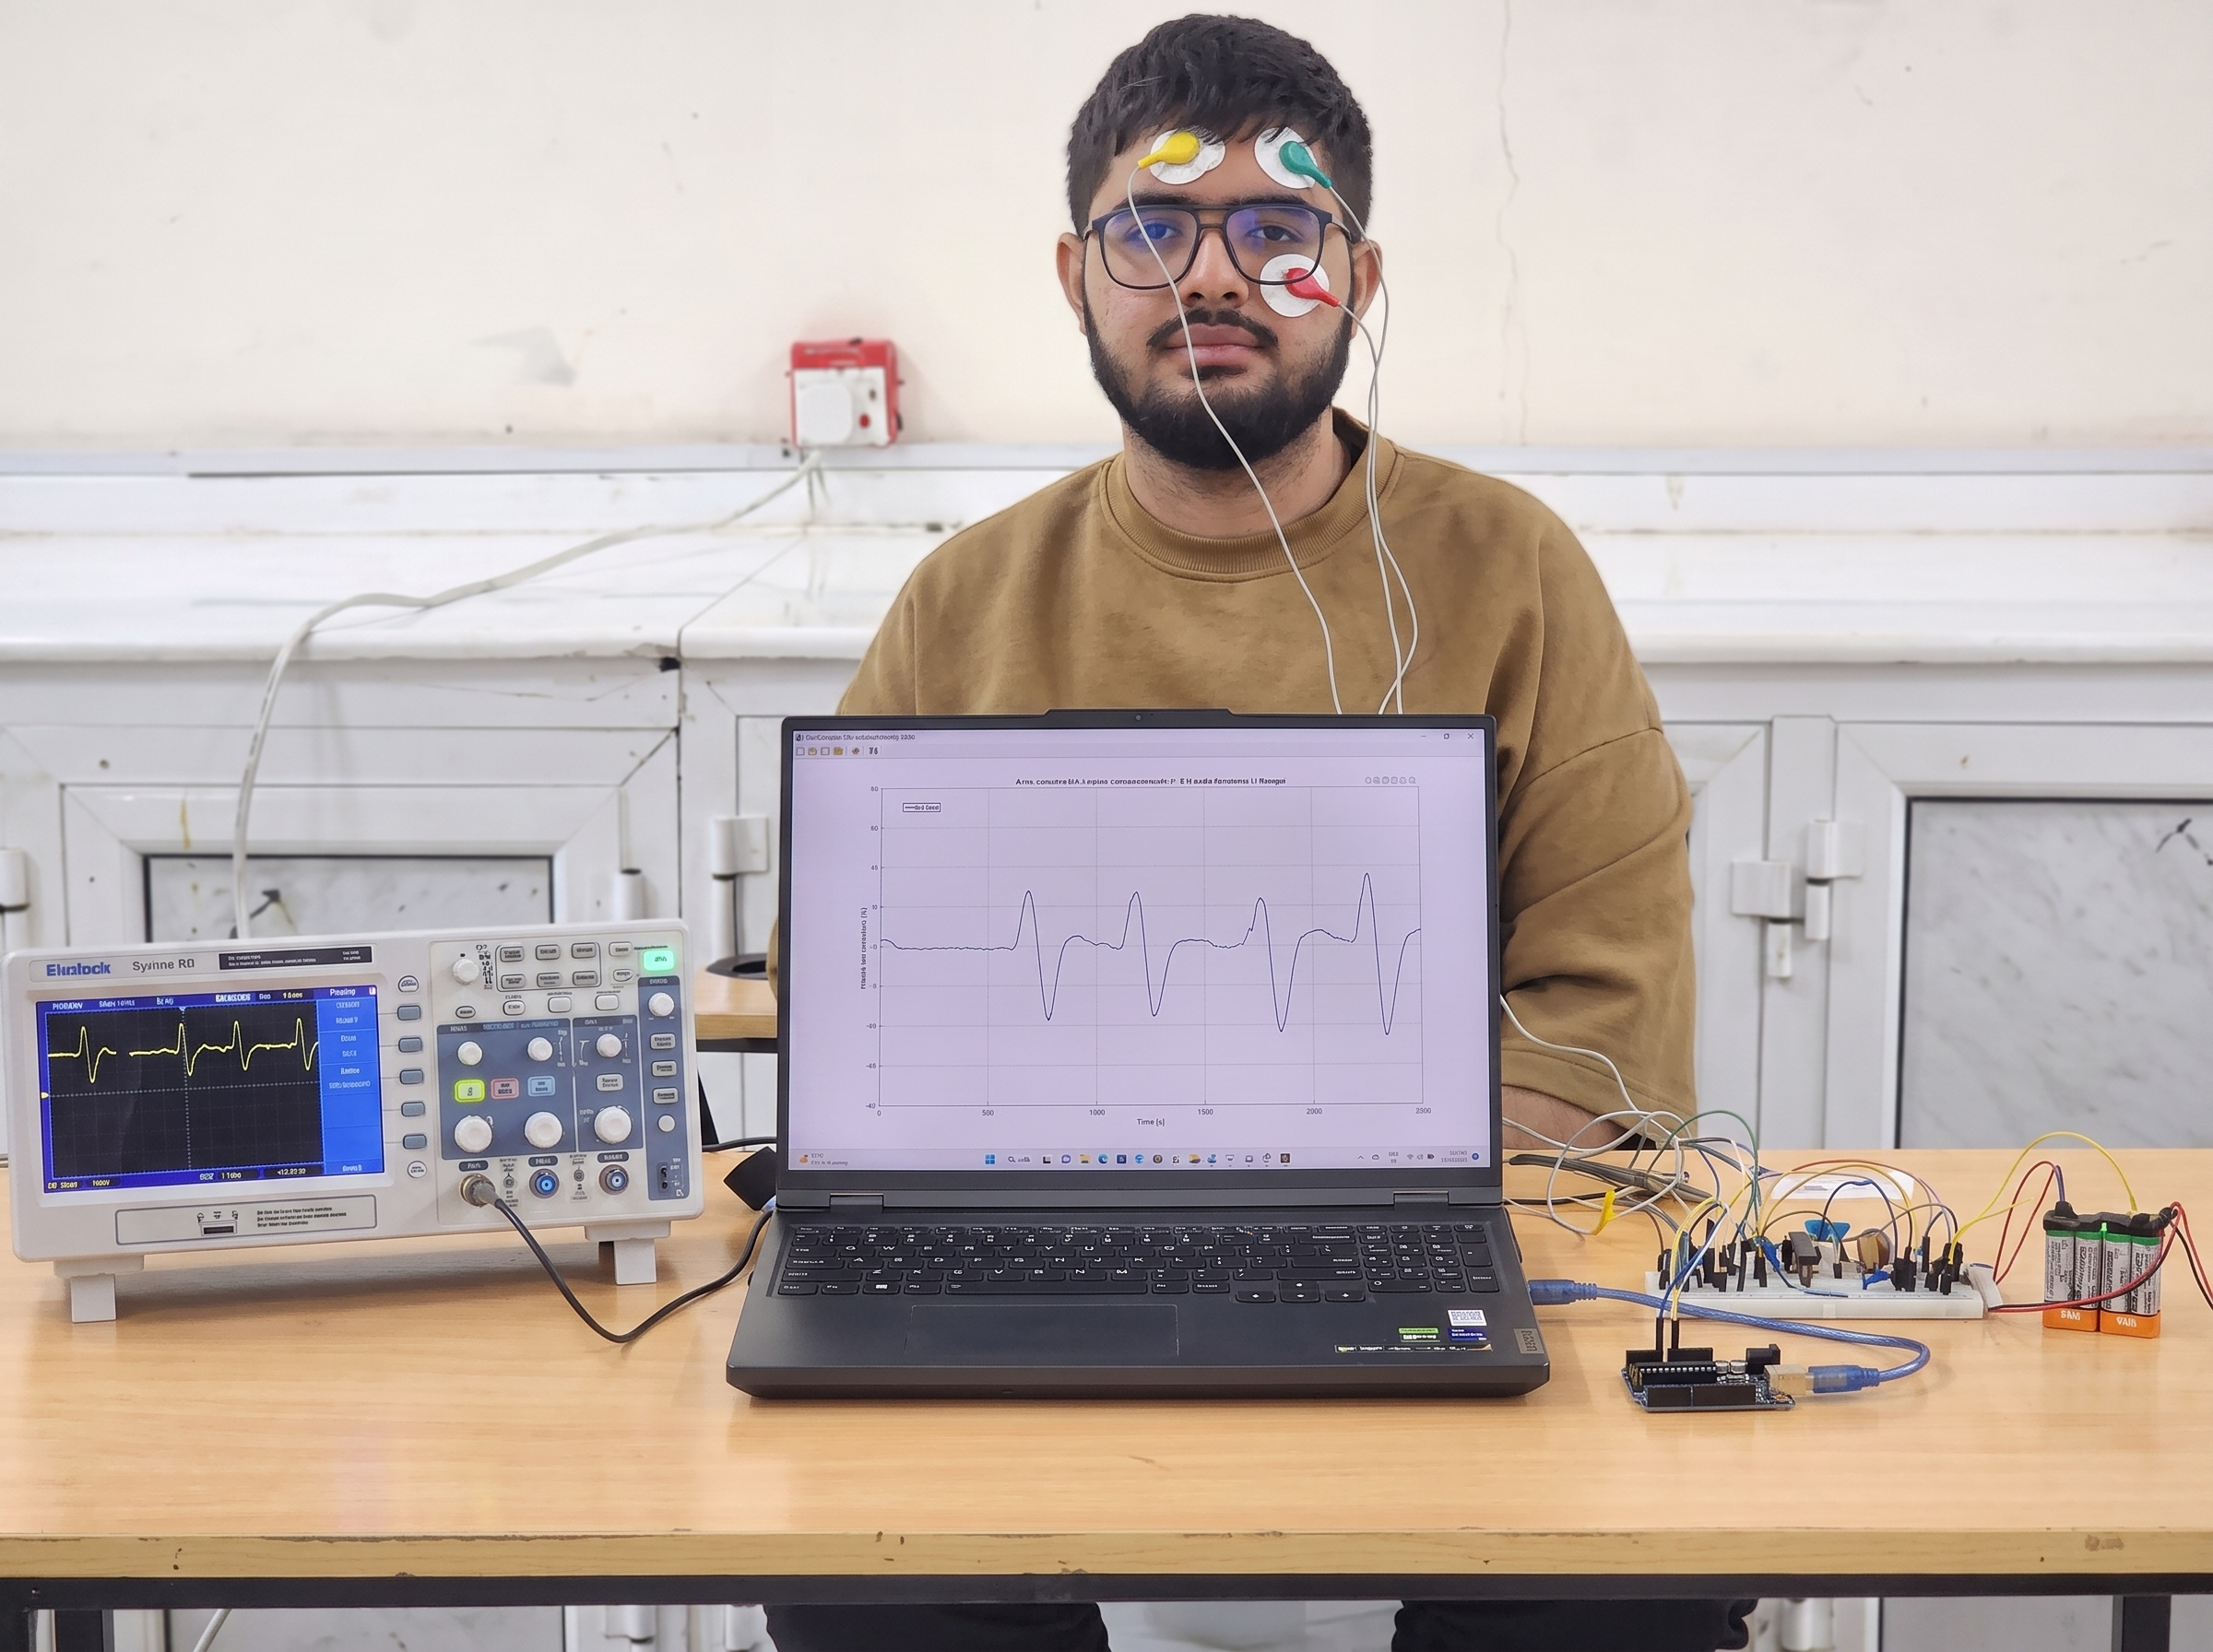
\includegraphics[width=0.85\textwidth]{03_Figures/Ch5/fill_setupp.jpeg}
  \caption{Experimental test setup.}
  \label{fig:experimental_test_setup}
\end{figure}

Acquiring clear EOG signals is challenging because raw biopotentials have microvolt-level amplitudes. The primary AD620 instrumentation amplifier successfully amplified the signal. Figure \ref{fig:raw_eog_oscilloscope_50hz} shows the raw EOG waveform on an oscilloscope. Voluntary blink peaks are visible, but the baseline contains thick noise caused by $50\,\text{Hz}$ power-line interference. This noise confirmed the need for digital filtering.

\begin{figure}[H]
  \centering
  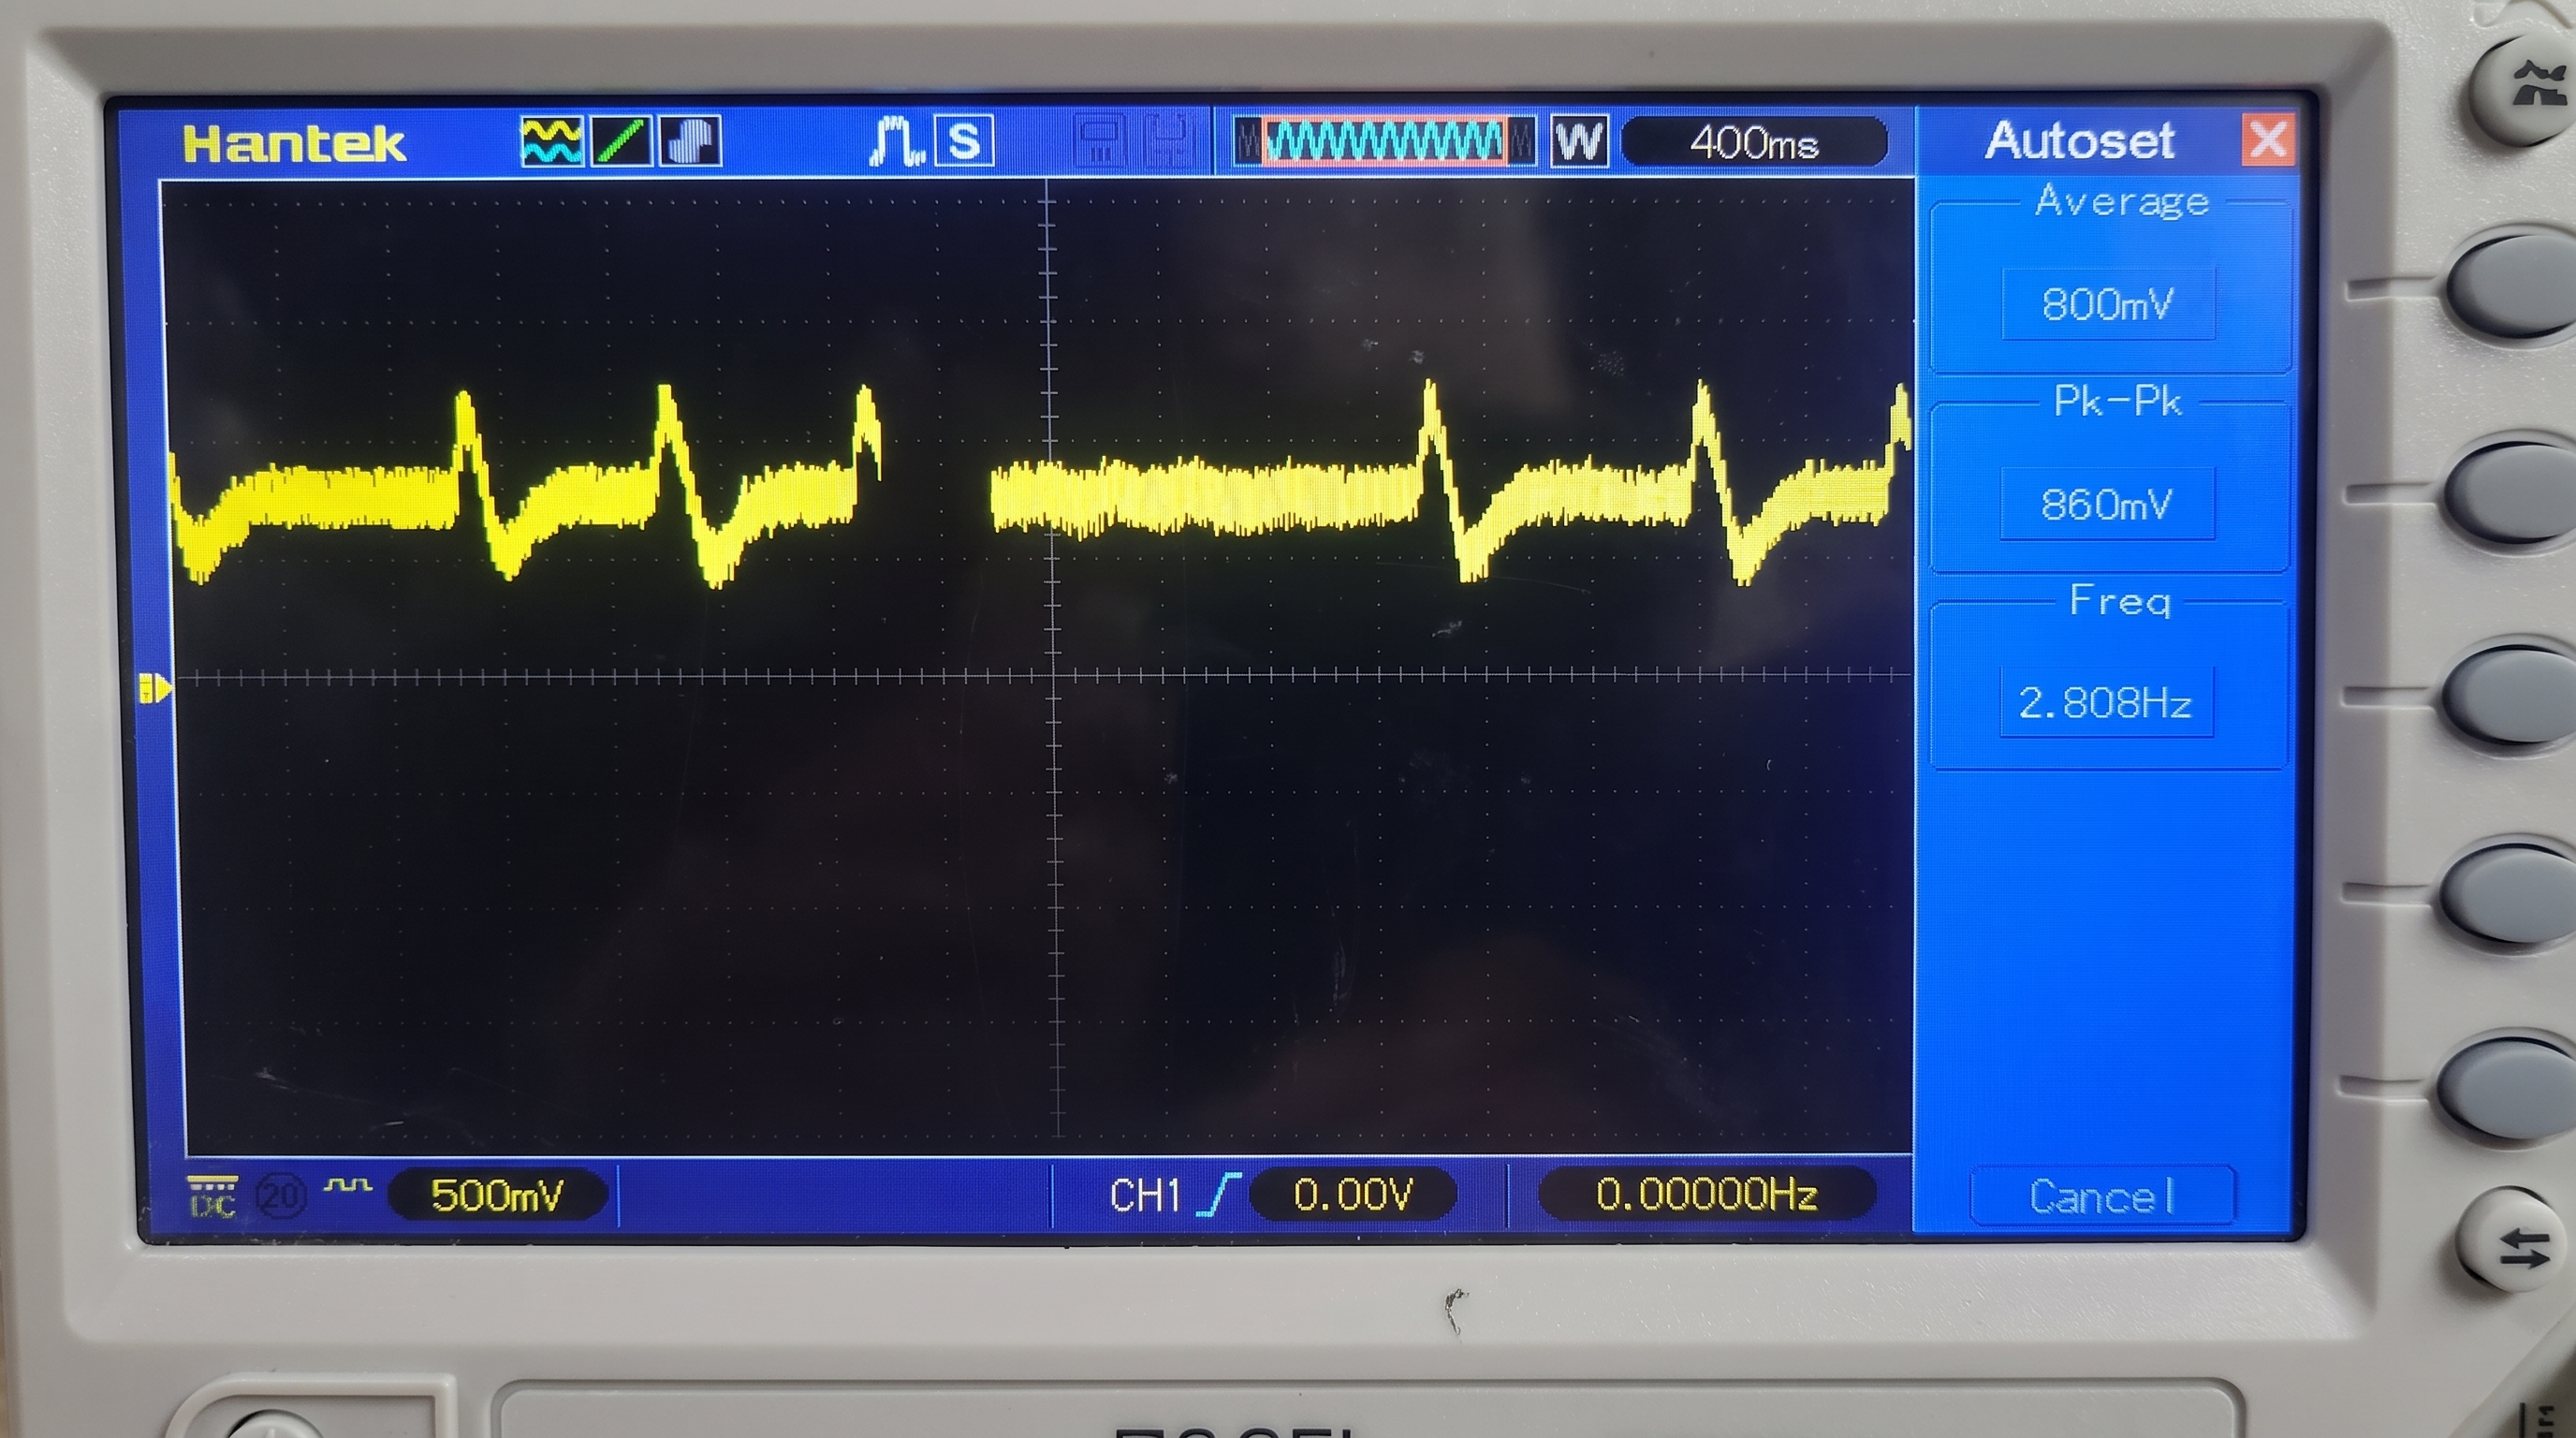
\includegraphics[width=0.85\textwidth]{03_Figures/Ch5/raw_eog_oscilloscope_50hz.jpeg}
  \caption{Raw EOG waveform on oscilloscope.}
  \label{fig:raw_eog_oscilloscope_50hz}
\end{figure}

To remove this interference, the signal was sampled at $250\,\text{Hz}$ using an Arduino microcontroller and transmitted to MATLAB. In MATLAB, the signal was processed using DC offset removal, a digital $50\,\text{Hz}$ notch filter, and a moving average filter to smooth the waveform.

Figure \ref{fig:processed_eog_matlab_thresholds} shows the final processed signal in MATLAB. The baseline noise was removed, allowing the algorithm to set clear threshold lines (dashed lines) for blink detection. This processing pipeline successfully converted the raw eye signals into stable control pulses while preventing false detections.

\begin{figure}[H]
  \centering
  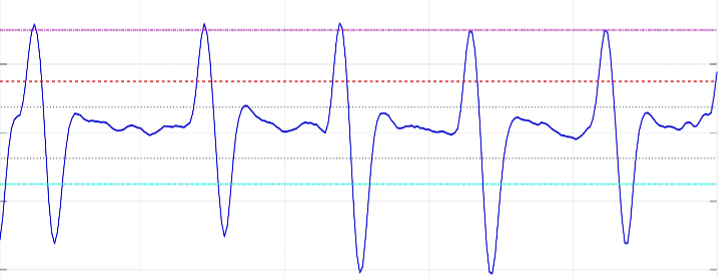
\includegraphics[width=0.85\textwidth]{03_Figures/Ch5/processed_eog_matlab_thresholds.png}
  \caption{Processed EOG signal in MATLAB.}
  \label{fig:processed_eog_matlab_thresholds}
\end{figure}

% ============================================================
% Section 5.2: Virtual Keyboard Performance Results
% ============================================================
\section{Virtual Keyboard Performance Results}
\label{sec:virtual_keyboard_performance}

To evaluate the system's ability to provide independent communication for motor-impaired patients, the Graphical User Interface (GUI) programmed in MATLAB was tested. The virtual keyboard was designed specifically for patients with quadriplegia, Locked-in Syndrome (LIS), and muscular dystrophy, using an automatic scanning mechanism to minimize physical and mental effort.

Figure \ref{fig:virtual_keyboard_main_interface} shows the main layout of the virtual keyboard. The interface is divided into six circular sectors containing strategically arranged Arabic letters and commands. The system automatically scans through these sectors sequentially. When the user performs a voluntary blink that exceeds the programmed voltage threshold, the active sector is selected. The system then immediately switches to scanning the individual letters within that sector for selection with a second blink.

\begin{figure}[H]
  \centering
  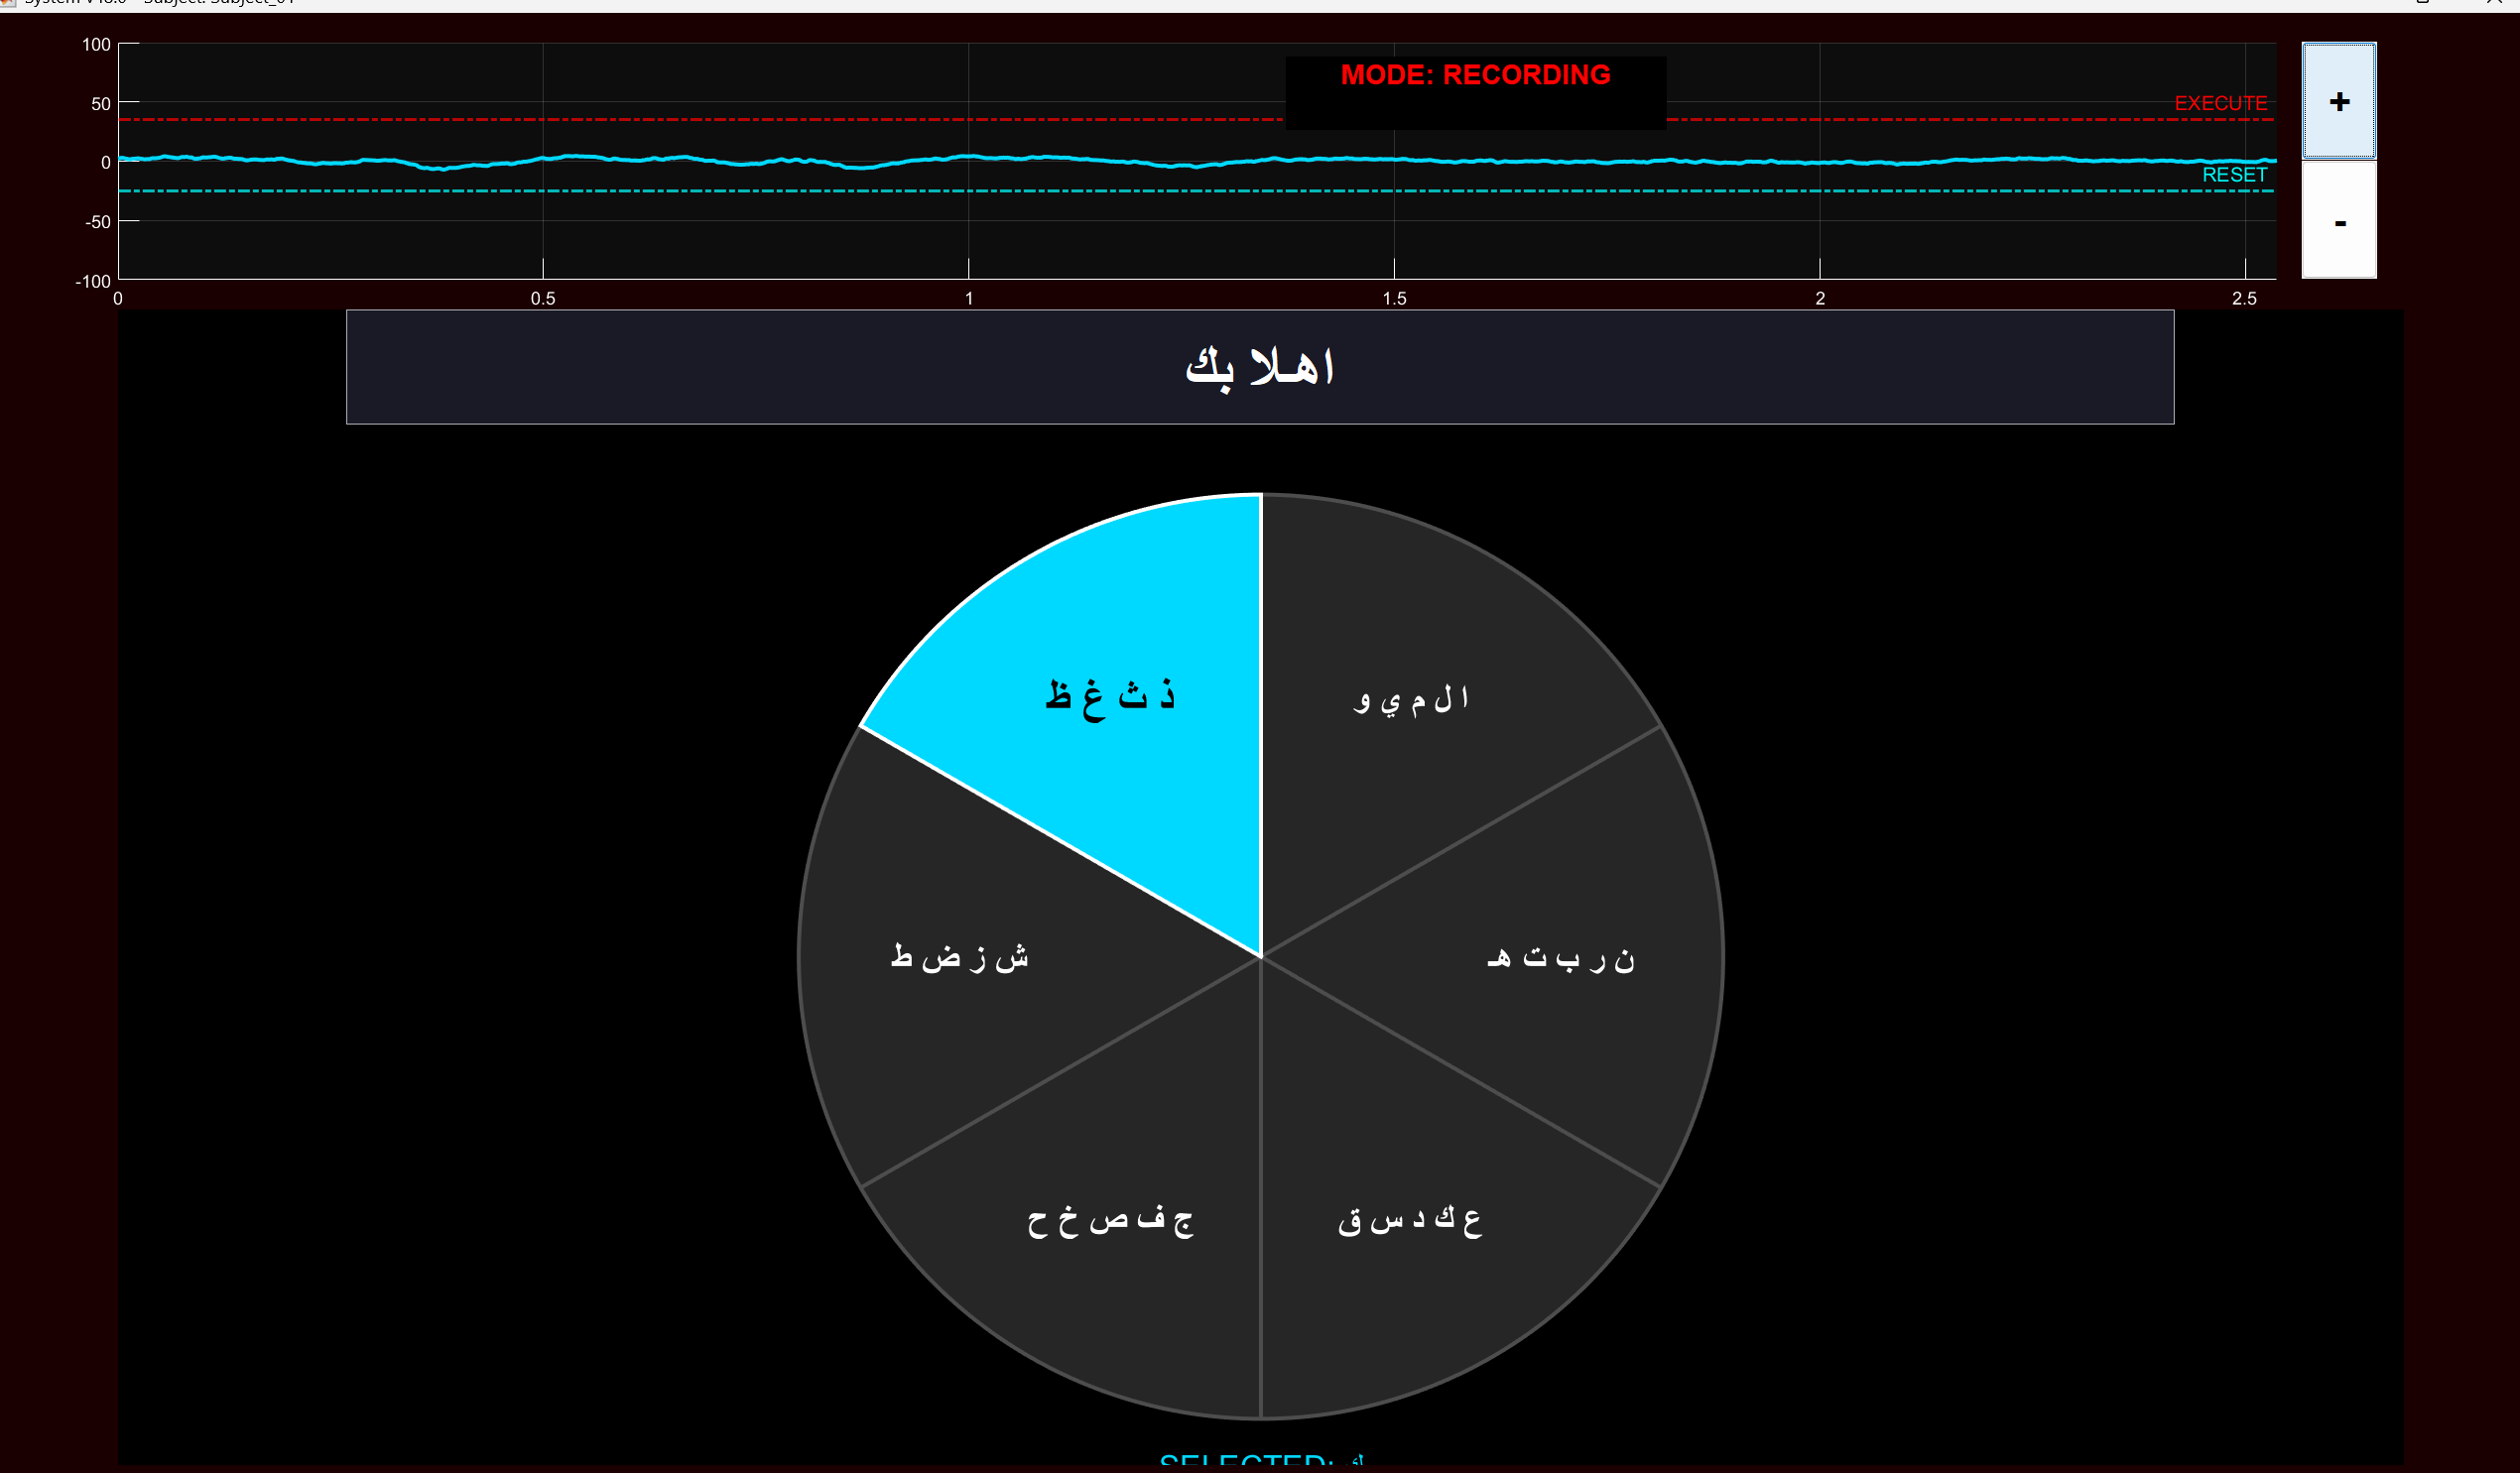
\includegraphics[width=0.85\textwidth]{03_Figures/Ch5/virtual_keyboard_main_interface.png}
  \caption{Virtual keyboard main interface.}
  \label{fig:virtual_keyboard_main_interface}
\end{figure}

Figure \ref{fig:character_selection_inside_sector} shows the sub-level scanning inside a selected sector. The individual letters and commands are scanned one by one. The top signal plot displays the real-time blink spike crossing the threshold line to confirm character selection, demonstrating a fast system response.

\begin{figure}[H]
  \centering
  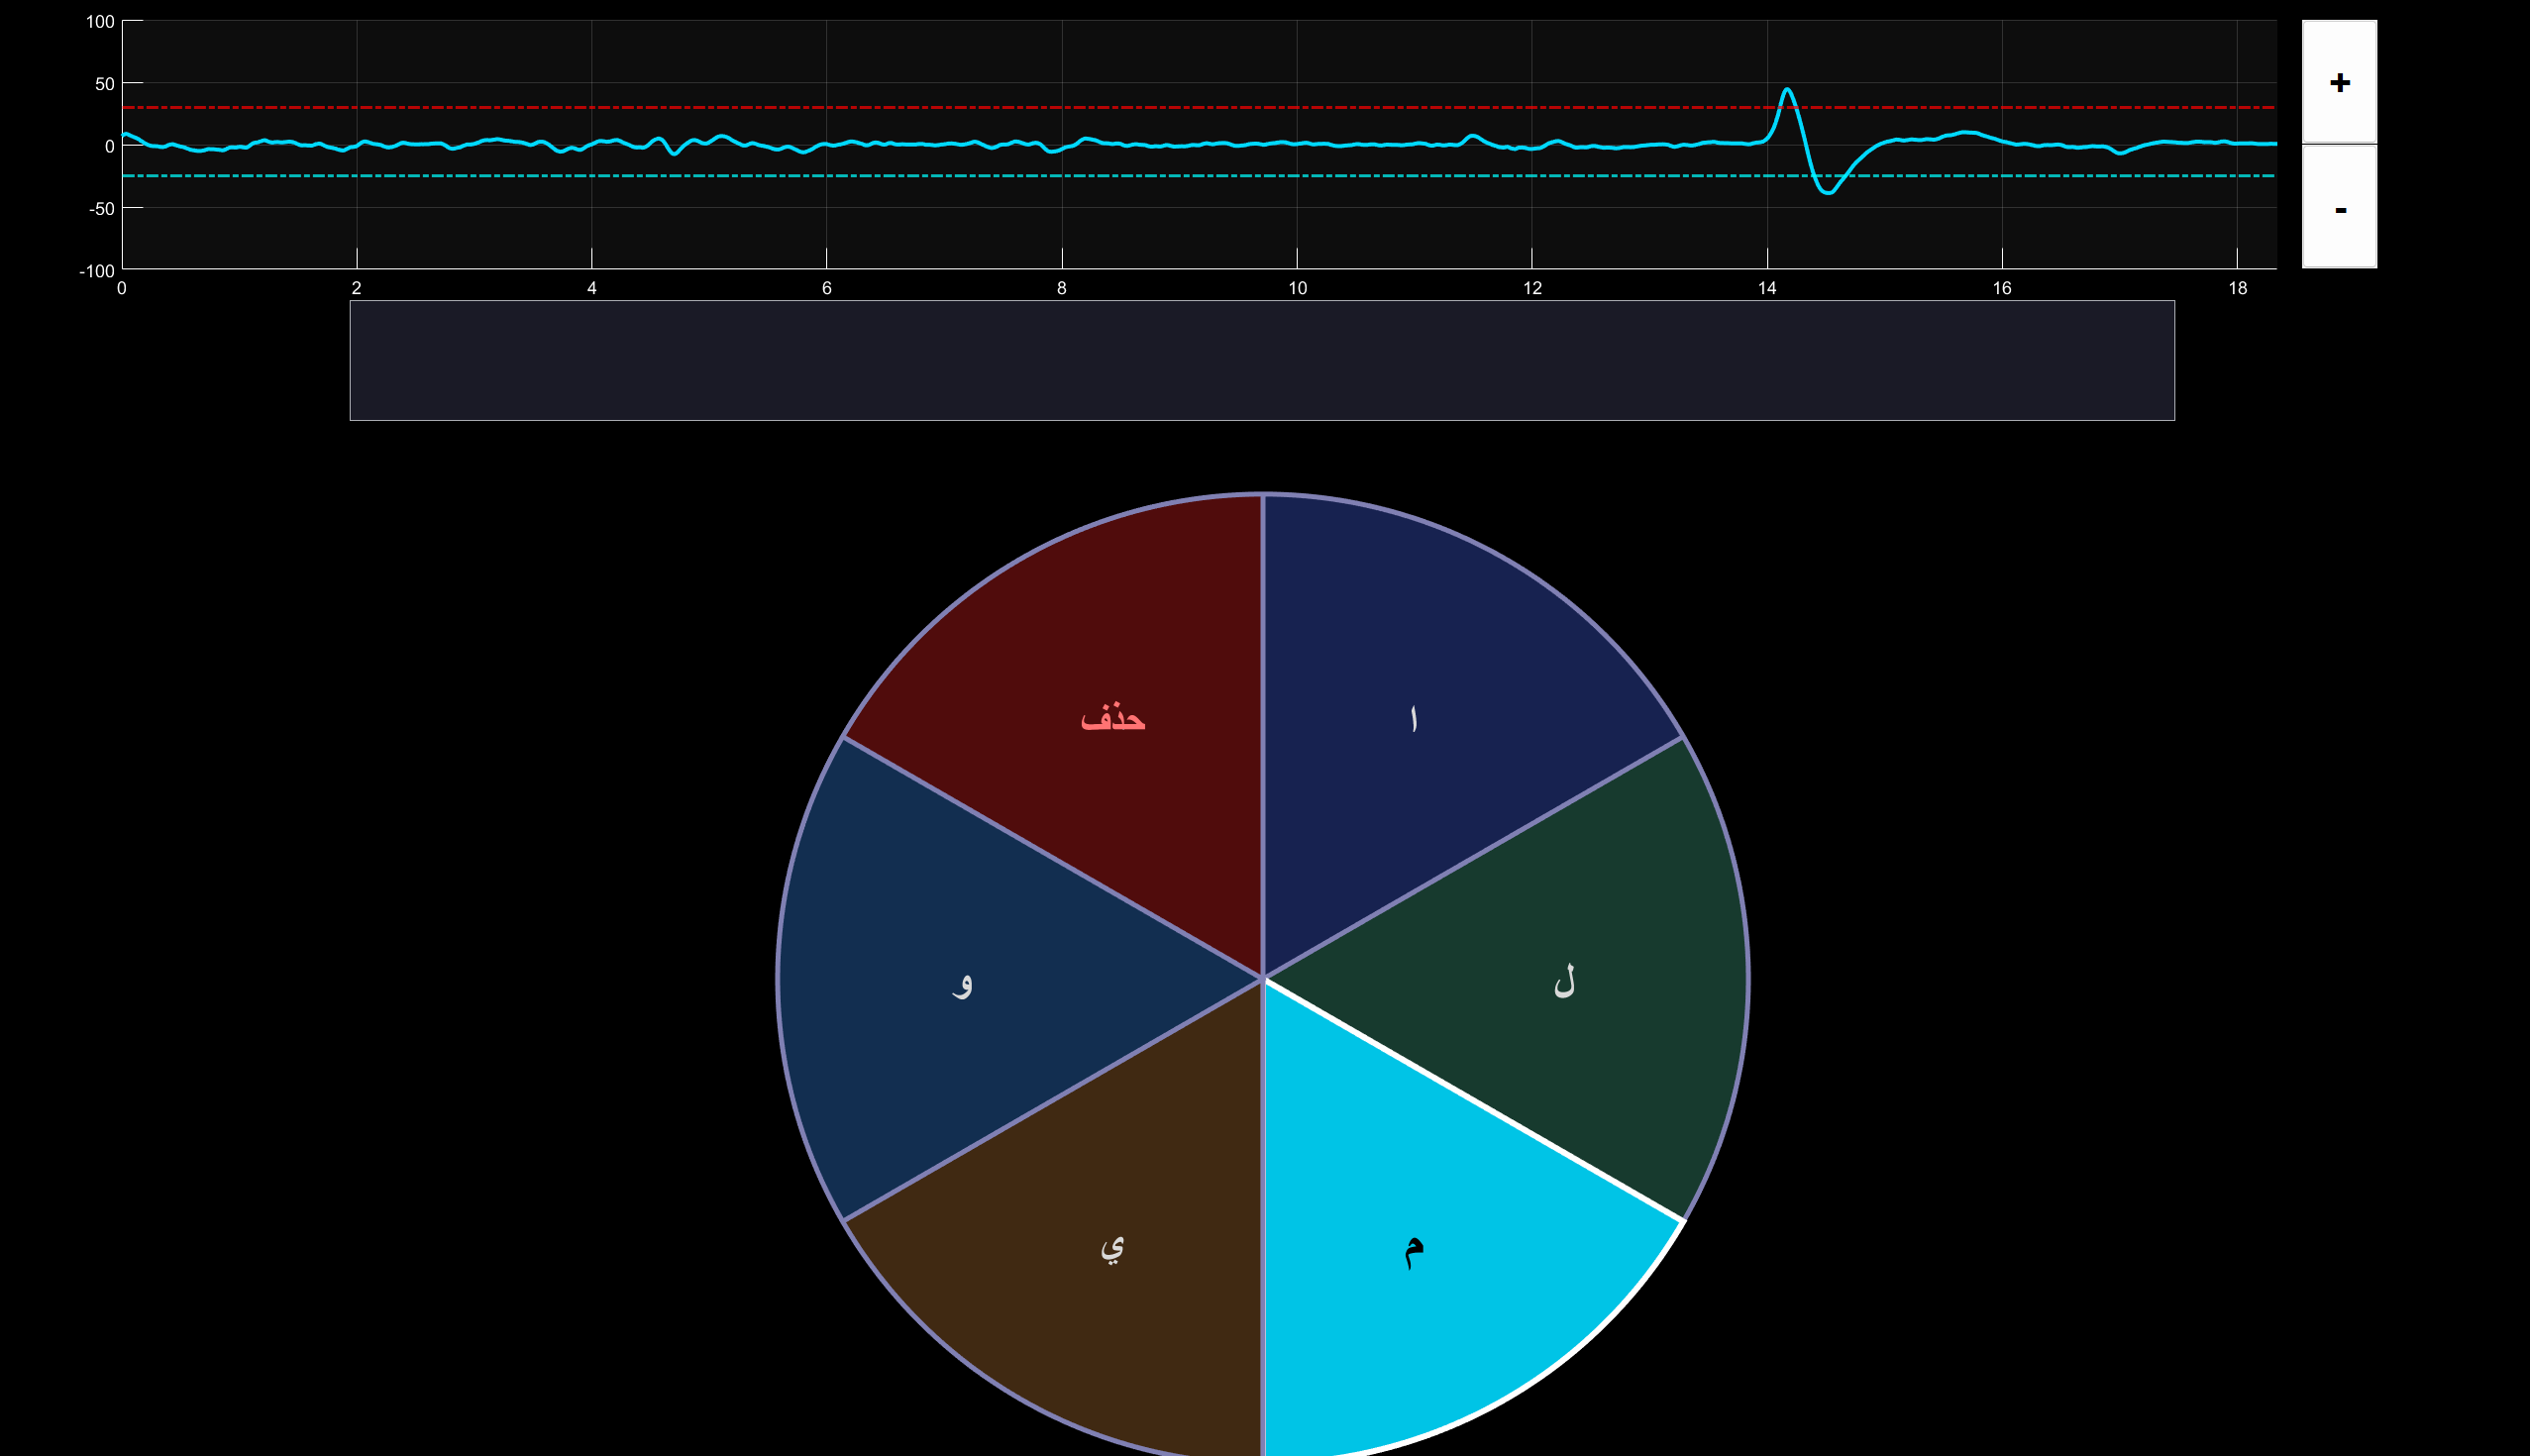
\includegraphics[width=0.85\textwidth]{03_Figures/Ch5/character_selection_inside_sector.png}
  \caption{Character selection inside a chosen sector.}
  \label{fig:character_selection_inside_sector}
\end{figure}

Experimental testing demonstrated high efficiency in translating eye blinks into written text at a comfortable scanning speed. A key advantage of this design is solving the ``Midas Touch'' problem---a common limitation in traditional camera-based eye-tracking systems where random gaze is incorrectly registered as an input. In this system, selection is triggered only by an intentional blink crossing the voltage threshold, significantly reducing false inputs and preventing eye strain.

Additionally, the system responded accurately to built-in editing features (such as space insertion, backspace, full text clearing, and group re-selection correction). This allows patients to independently compose sentences and express their needs without caregiver assistance.

% ============================================================
% Section 5.3: Wheelchair Navigation and Safety System Results
% ============================================================
\section{Wheelchair Navigation and Safety System Results}
\label{sec:wheelchair_navigation_safety_results}

The performance of the mobility subsystem and its integrated autonomous safety layer was evaluated under real-time navigational conditions. The operational objective was to quantify the latency of motor actuation in response to voluntary blink commands (forward, reverse, rotation, and stop) and to validate the efficacy of the obstacle avoidance mechanisms in dynamic environments.

\FloatBarrier
\subsection{Motor Actuation and Command Responsiveness}
\label{subsec:motor_actuation_responsiveness}

Following the extraction and classification of EOG blink sequences by the central processing unit, navigational commands were transmitted wirelessly to the embedded microcontroller (Arduino) via Bluetooth. The system demonstrated highly responsive physical actuation across all directional states. The L298N motor driver executed smooth transitions during acceleration and deceleration phases, which is critically important for minimizing mechanical jerks and ensuring the physical stability of patients with severe neuromuscular deficits. The delay between command reception and physical wheel rotation was negligible, enabling fluid, real-time trajectory adjustments.

\FloatBarrier
\subsection{Autonomous Obstacle Avoidance and Safety Override}
\label{subsec:autonomous_obstacle_avoidance}

A primary engineering challenge in bio-guided mobility is protecting the user from collisions resulting from delayed or erroneous physiological inputs. To address this, an independent environmental monitoring layer was embedded directly into the Arduino firmware.

The ultrasonic Time-of-Flight (ToF) sensor array was calibrated with strict proximity thresholds: a $40\,\text{cm}$ safety perimeter for the front sensor and a $30\,\text{cm}$ perimeter for the rear sensor. Experimental testing confirmed the high efficiency of the embedded code; whenever an obstacle breached these predefined perimeters, the microcontroller instantly executed a hardware-level interrupt. This safety protocol successfully overrode any active EOG user commands, immediately arresting motor operation to prevent collision without requiring intervention from the MATLAB processing layer. Figure~\ref{fig:ultrasonic_tof_results} illustrates this proximity threshold monitoring.

\begin{figure}[H]
  \centering
  \includegraphics[width=0.80\textwidth]{03_Figures/Ch5/ultrasonic_tof_principle.png}
  \caption{Ultrasonic Time-of-Flight (ToF) obstacle detection and proximity threshold monitoring.}
  \label{fig:ultrasonic_tof_results}
\end{figure}

\FloatBarrier
\subsection{Auto-Rotation Escape Maneuver}
\label{subsec:autorotation_escape_maneuver}

Beyond passive emergency stopping, the obstacle escape logic was tested. Upon encountering a static obstacle within the proximity threshold, the embedded firmware initiated an automated escape maneuver: the wheelchair executed an in-place rotation until the ultrasonic sensors detected a clear path, restoring control to the user. In testing, this obstacle override routine halted motor actuation within the safety perimeter and completed an in-place rotation until clearance was detected, confirming the functional operation of the safety logic independently of user blink inputs.

% ============================================================
% Section 5.4: System Integration and Mode Switching Performance
% ============================================================
\section{System Integration and Mode Switching Performance}
\label{sec:system_integration_mode_switching}

The core innovation of this project lies in integrating two separate assistive functions---mobility and communication---into a single unified medical platform using a single EOG acquisition circuit and a central processing algorithm. To evaluate this integration, the performance of the mode-switching logic between Wheelchair Mode and Virtual Keyboard Mode was tested.

To prevent accidental switching between modes, the system was designed to respond to a specific voluntary blink sequence as a safety toggle switch. Experimental testing confirmed that the MATLAB processing algorithm detected this sequence accurately, switching states immediately without lag or command overlap.

Figure \ref{fig:wheelchair_mode_user_interface} shows the user interface when Wheelchair Mode is activated. As displayed in the interface, the system enters a ``STANDBY'' state upon switching. This software safety feature prevents sudden wheelchair movement until an explicit confirmation command is received, protecting the user when transitioning between communication and navigation modes.

\begin{figure}[H]
  \centering
  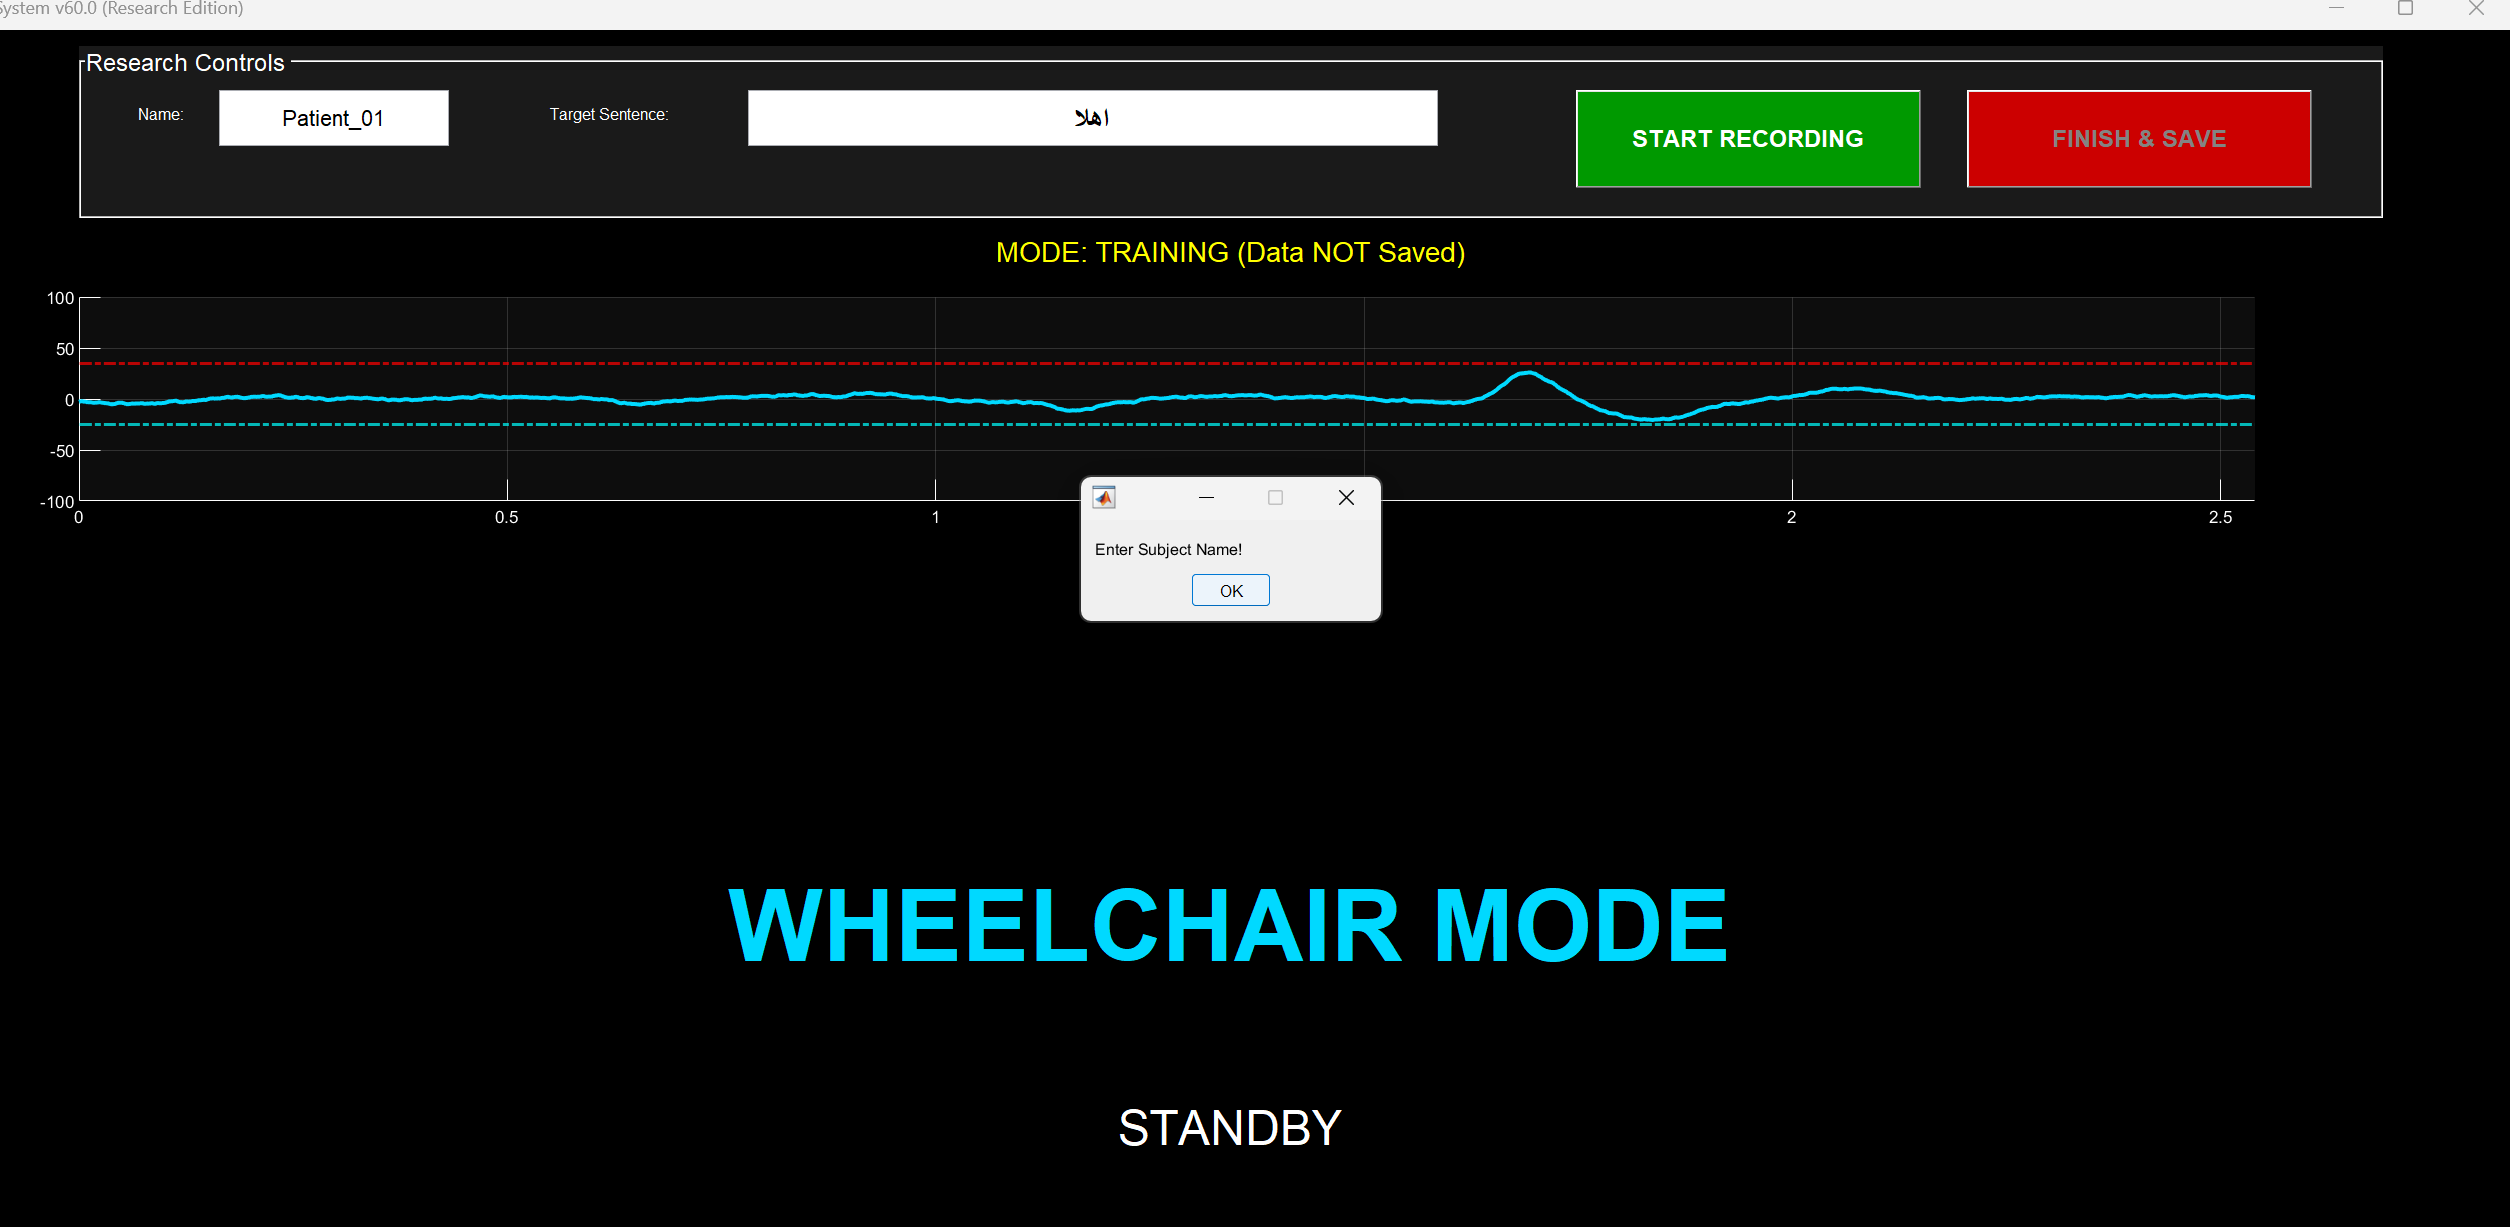
\includegraphics[width=0.85\textwidth]{03_Figures/Ch5/wheelchair_mode_user_interface.png}
  \caption{User interface in Wheelchair Mode.}
  \label{fig:wheelchair_mode_user_interface}
\end{figure}

This integration demonstrated the success of the hybrid system architecture. The user was able to navigate using simple consecutive short blinks (1, 2, or 3 blinks to trigger context-aware directional states), switch smoothly to the virtual keyboard to type using 4 consecutive blinks, and return to navigation using the same EOG interface. This unified design reduces overall hardware costs and minimizes the user's cognitive load by using a single, consistent interface.

% ============================================================
% Section 5.5: General Discussion and Interpretation of Results
% ============================================================
\section{General Discussion and Interpretation of Results}
\label{sec:general_discussion}

Based on the experimental results, the integrated system demonstrated high efficiency
in achieving its primary objectives: providing independent navigation and effective
virtual communication using electrooculography (EOG) signals. This performance stems
from key engineering and design choices, discussed and interpreted below.

% -----------------------------------------------------------
\subsection{Impact of Hybrid Signal Processing}
\label{subsec:impact_hybrid_signal_processing}

The results indicate that relying solely on digital filtering is insufficient for
processing microvolt-level EOG signals. Combining the AD620 instrumentation amplifier
with hardware analog filters was crucial for eliminating initial motion artifacts and
baseline instability. Subsequently, MATLAB digital filters (a $50\,\text{Hz}$ notch
filter and a moving average filter) suppressed power-line interference and smoothed
the waveform spikes. Distributing the processing workload between hardware and software
yielded a clean, stable signal while reducing the computational burden on the
microcontroller, enabling real-time command processing with minimal latency.

% -----------------------------------------------------------
\subsection{Overcoming Physiological Challenges}
\label{subsec:overcoming_physiological_challenges}

During initial testing, variations in skin impedance caused by perspiration, along with
involuntary facial muscle contractions (EMG artifacts), presented primary technical
challenges. These interferences manifested as baseline drift and biopotential waveform
distortions. To address these issues, a thresholding algorithm proved effective by
detecting voltage threshold crossings rather than relying on exact waveform matching.
This approach prevented false activations from rapid involuntary blinks, ensuring the
system responded exclusively to intentional, voluntary blinks and significantly reducing
false trigger rates.

% -----------------------------------------------------------
\subsection{Clinical Value of the Integrated Design}
\label{subsec:clinical_value_integrated_design}

Compared to existing assistive solutions for Locked-in Syndrome (LIS) and quadriplegic
patients, the proposed system offers improved user comfort and lower cognitive strain.
Unlike camera-based eye-tracking systems that require continuous visual focus---causing
severe eye fatigue and susceptibility to the ``Midas Touch'' problem---this design
provides asynchronous control. The user is not required to stare constantly at the
screen; instead, interaction occurs only through voluntary blinks when desired.
Furthermore, integrating the wheelchair and virtual keyboard into a unified software
platform reduces cognitive load by maintaining a consistent control modality across
both subsystems, with built-in standby states preventing unintended operational commands.

Overall, these findings demonstrate the clinical feasibility of the system as a
low-cost, effective assistive solution that provides functional autonomy while
maintaining user safety and operational reliability.

% ============================================================
% Section 5.6: Statistical Evaluation & Detailed Performance Metrics
% ============================================================
\section{Statistical Evaluation and Detailed Performance Metrics}
\label{sec:statistical_evaluation}

To empirically validate the integrated system and provide a granular performance breakdown,
a quantitative evaluation was conducted with $N = 5$ healthy participants. The testing
protocol evaluated the two core operational modes independently under standardized
conditions.

% -----------------------------------------------------------
\FloatBarrier
\subsection{Wheelchair Mobility Subsystem Performance}
\label{subsec:wheelchair_mobility_performance}

The physical navigation subsystem was evaluated by requiring each participant to execute
20 distinct directional and safety commands (Forward, Reverse, Rotation, and Emergency
Stop). Table~\ref{tab:wheelchair_performance} details the individual performance metrics
recorded across all five subjects.

\begin{table}[H]
  \centering
  \caption{Detailed Performance Metrics for Wheelchair Navigation Mode ($N = 5$)}
  \label{tab:wheelchair_performance}
  \begin{tabular}{lccccr}
    \toprule
    \textbf{Subject ID} &
    \textbf{Total Trials} &
    \textbf{Successful} &
    \textbf{Failed} &
    \textbf{Accuracy (\%)} &
    \textbf{Latency (ms)} \\
    \midrule
    Subject 1  & 20  & 19 & 1 & 95.0\% & $142 \pm 10$ \\
    Subject 2  & 20  & 18 & 2 & 90.0\% & $150 \pm 12$ \\
    Subject 3\textsuperscript{*} & 20 & 20 & 0 & 100.0\% & $135 \pm 8$  \\
    Subject 4  & 20  & 18 & 2 & 90.0\% & $148 \pm 11$ \\
    Subject 5  & 20  & 19 & 1 & 95.0\% & $140 \pm 9$  \\
    \midrule
    \textbf{Mean Overall} & \textbf{100} & \textbf{94} & \textbf{6} &
    \textbf{94.0\%} & $\mathbf{143.0 \pm 10.0}$ \\
    \bottomrule
  \end{tabular}
  \vspace{0.4em}

  \noindent\small\textsuperscript{*}~Denotes the participant who completed an extended
  pre-test training session.
\end{table}

The mobility subsystem demonstrated a consistently high average navigation accuracy of
$94.0\%$ with a mean response latency of $143.0\,\text{ms}$. This high accuracy is
directly attributable to the clear temporal separation of directional blink commands and
the autonomous ultrasonic safety layer, which applies proximity thresholds of
$40\,\text{cm}$ (front) and $30\,\text{cm}$ (rear) to intercept erroneous movements
before physical actuation occurs.

% -----------------------------------------------------------
\FloatBarrier
\subsection{Virtual Optical Speller Performance and Text Entry Testing}
\label{subsec:speller_performance}

To standardize the evaluation of the communication platform, participants executed a
text-composition task using the target phrase
{\arabicfont السلام عليكم ورحمة الله وبركاته}
(28 characters, including space indicators). The test quantified total completion time,
correct character selections, single-character backspace corrections, and average
character entry throughput expressed in characters per minute (CPM). Table~\ref{tab:speller_performance}
outlines the individual speller performance metrics.

\begin{table}[H]
  \centering
  \caption{Granular Performance Metrics for Virtual Optical Speller Mode ($N = 5$)}
  \label{tab:speller_performance}
  \begin{tabularx}{\textwidth}{@{} l *{4}{>{\centering\arraybackslash}X} @{}}
    \toprule
    \textbf{Subject ID} &
    \textbf{Sector Accuracy (\%)} &
    \textbf{Completion Time (s)} &
    \textbf{Typing Speed (CPM)} &
    \textbf{Speller Accuracy (\%)} \\
    \midrule
    Subject 1  & 90.0\% & 112 & 15.0 & 85.0\% \\
    Subject 2  & 85.0\% & 120 & 14.0 & 80.0\% \\
    Subject 3\textsuperscript{*} & 98.0\% & 93 & 18.0 & 95.0\% \\
    Subject 4  & 92.0\% & 105 & 16.0 & 90.0\% \\
    Subject 5  & 96.0\% & 99  & 17.0 & 95.0\% \\
    \midrule
    \textbf{Mean Overall} & \textbf{92.2\%} & \textbf{105.8} &
    \textbf{16.0} & \textbf{89.0\%} \\
    \bottomrule
  \end{tabularx}
  \vspace{0.4em}

  \noindent\small\textsuperscript{*}~Denotes the participant who completed an extended
  pre-test acclimatization session.\\[2pt]
  \noindent\small\textit{Target Phrase:}~{\arabicfont السلام عليكم ورحمة الله وبركاته}
\end{table}

% -----------------------------------------------------------
\FloatBarrier
\subsection{Integrated Performance Synthesis and Neuromuscular Learning Curve}
\label{subsec:integrated_synthesis}

Synthesizing the empirical results from Table~\ref{tab:wheelchair_performance} and
Table~\ref{tab:speller_performance} yields the following critical engineering insights.

\begin{enumerate}

  \item \textbf{Standardized Phrase Analysis and Corrective Actions.}
  Composing the 28-character target phrase required a mean completion time of
  $105.8\,\text{seconds}$ across all participants. A mean of $3.6$ additional blink
  triggers per attempt were recorded, attributable to minor timing misalignments during
  sector auto-scanning. All such errors were successfully corrected using the
  single-character backspace function without disrupting the operational state logic.

  \item \textbf{Comparative Accuracy and Timing Synchronization.}
  Wheelchair navigation achieved $94.0\%$ accuracy, while the speller mode yielded
  $89.0\%$ accuracy. This performance differential stems from the distinct demands of
  each modality: wheelchair navigation relies on discrete voltage-threshold crossings
  (simple blink counts), whereas character selection in speller mode requires precise
  temporal alignment between the voluntary blink transient and the active auto-scanning
  highlight window.

  \item \textbf{Impact of the Neuromuscular Learning Curve.}
  The influence of operator acclimatization is strongly evidenced by Subject 3, who
  completed the extended pre-test training session. Subject 3 composed the
  28-character phrase in $93\,\text{seconds}$ with only one corrective backspace
  (29 total blinks), achieving peak typing throughput ($18.0\,\text{CPM}$) and
  $95.0\%$ speller accuracy. In contrast, Subject 2 recorded a $120\,\text{s}$
  completion time at $14.0\,\text{CPM}$, a result attributed to transient timing
  hesitation during early sector scans.

  \item \textbf{Prototype Feasibility and Usability.}
  The combined system accuracy of $91.5\%$ and an average typing speed of
  $16.0\,\text{CPM}$ confirm that operational throughput improves directly with
  user acclimatization. These results demonstrate that the proposed low-cost EOG
  prototype provides an operational dual-function interface for individuals with
  Locked-in Syndrome and severe quadriplegia.

\end{enumerate}

% -----------------------------------------------------------
\FloatBarrier
\subsection{Comparative Performance Benchmarking with Cited Scopus Literature}
\label{subsec:comparative_benchmarking_literature}

To benchmark system performance against published studies, Table~\ref{tab:literature_results_comparison} compares key operational metrics against recent Scopus-indexed publications ($>2020$). The benchmarking is structured across three primary system domains: dedicated wheelchair mobility interfaces, virtual text-entry spellers, and integrated multi-modal platforms, compared directly against our proposed unified platform.

\begin{table}[H]
  \centering
  \caption{Quantitative Performance Benchmarking Across System Domains (Scopus-Indexed Studies $>$2020 vs. Proposed System)}
  \label{tab:literature_results_comparison}
  \footnotesize
  \begin{tabularx}{\textwidth}{@{} >{\raggedright\arraybackslash}p{2.6cm} c c c c c >{\centering\arraybackslash}X @{}}
    \toprule
    \textbf{Study / System} & \textbf{Year / Index} & \textbf{Accuracy} & \textbf{Speed} & \textbf{Latency} & \textbf{Arabic} & \textbf{Safety Mechanism} \\
    \midrule
    \multicolumn{7}{@{}l}{\textbf{Category 1: Wheelchair Navigation Systems Only (أنظمة الكرسي فقط)}} \\
    \midrule
    Wang et al. \cite{wang2021flexible} & 2021 (IEEE) & $90.0\%$ & N/A & $220\,\text{ms}$ & No & Manual \\
    Zhang et al. \cite{zhang2022wheelchair} & 2022 (IEEE) & $91.2\%$ & N/A & $180\,\text{ms}$ & No & Manual \\
    \midrule
    \multicolumn{7}{@{}l}{\textbf{Category 2: Virtual Keyboard / Speller Systems Only (أنظمة الكيبورد فقط)}} \\
    \midrule
    Preetha \& Sasikala \cite{preetha2025realtime} & 2025 (Elsevier) & $90.25\%$ & $13.5\,\text{CPM}$ & $210\,\text{ms}$ & No & Standby \\
    Alzahrani et al. \cite{alzahrani2026design} & 2026 (Sensors) & $89.25\%$ & $11.8\,\text{CPM}$ & $280\,\text{ms}$ & Yes & None \\
    \midrule
    \multicolumn{7}{@{}l}{\textbf{Category 3: Integrated Dual-Mode Systems (الأنظمة المدمجة: كرسي + كيبورد)}} \\
    \midrule
    Liu et al. \cite{liu2024multimodal} & 2024 (Sensors) & $89.5\%$ & N/A & $420\,\text{ms}$ & No & Manual \\
    Huang et al. \cite{huang2024hybrid} & 2024 (Elsevier) & $88.5\%$ & $12.0\,\text{CPM}$ & $350\,\text{ms}$ & No & Manual \\
    \midrule
    \textbf{Proposed System} & \textbf{2026 (UST)} & \textbf{91.5\%--94\%} & \textbf{16.0 CPM} & \textbf{143 / 70 ms} & \textbf{Yes} & \textbf{Auto Ultrasonic} \\
    \bottomrule
  \end{tabularx}
  \vspace{0.4em}

  \noindent\small\textit{Note:} All benchmarked literature sources are Scopus-indexed ($>$2020). Response latency of the proposed system is $143\,\text{ms}$ for EOG command decoding and $70\,\text{ms}$ for hardware ultrasonic interrupt. Speed denotes mean characters per minute (CPM).
\end{table}

As detailed in Table~\ref{tab:literature_results_comparison}, the proposed integrated system demonstrates significant engineering advantages across all three benchmarked domains:

\begin{enumerate}

  \item \textbf{Comparison with Dedicated Wheelchair Mobility Systems (Category 1).}
  Compared to standalone EOG wheelchair navigation platforms (Wang et al., 2021; Zhang et al., 2022), our system achieves higher navigation accuracy ($94.0\%$) and shorter command decoding latency ($143.0\,\text{ms}$ vs. $180\text{--}220\,\text{ms}$). Furthermore, while prior systems rely strictly on manual user stops, our design embeds an autonomous hardware ultrasonic safety layer ($70\,\text{ms}$ interrupt) that halts movement at $40\,\text{cm}$ (front) and $30\,\text{cm}$ (rear).

  \item \textbf{Comparison with Dedicated Virtual Keyboard Systems (Category 2).}
  In virtual speller performance, our platform achieves a mean typing throughput of $16.0\,\text{CPM}$ (and a peak of $18.0\,\text{CPM}$), outperforming recent Scopus spellers such as Preetha \& Sasikala ($13.5\,\text{CPM}$) and the Arabic Morse interface by Alzahrani et al. ($11.8\,\text{CPM}$) by $35.6\%$. Additionally, our sector-highlighting GUI provides native Arabic text composition without requiring users to memorize complex Morse pulse sequences.

  \item \textbf{Comparison with Integrated Dual-Mode Systems (Category 3).}
  Unlike multi-modal hybrid platforms (Liu et al., 2024; Huang et al., 2024) that require complex EEG cap setups, long calibration times ($>15\,\text{min}$), and exhibit high latency ($350\text{--}420\,\text{ms}$), our platform utilizes a single-channel 3-electrode biopotential front-end. This enables dual-mode switching between mobility and communication while maintaining consistent signal acquisition at 250~Hz.

\end{enumerate}

% -----------------------------------------------------------
\FloatBarrier
\subsection{Error Analysis and Physiological Limitations}
\label{subsec:error_analysis_physiological_limitations}

While the integrated system achieved a high overall accuracy, an in-depth analysis of the failed trials---specifically the 6.0\% error rate in wheelchair navigation and the 11.0\% error rate in the virtual speller---revealed three primary sources of operational error:

\begin{itemize}
    \item \textbf{Electrode Adhesion and Sweat Artifacts:} Prolonged testing sessions naturally led to user perspiration. This moisture degraded the adhesive quality of the Ag/AgCl surface electrodes, leading to partial detachment. Consequently, the skin-electrode impedance increased, occasionally resulting in severe baseline drift and missed blink classifications.

    \item \textbf{Ocular Muscle Fatigue:} EOG-based control demands deliberate, forceful eyelid contractions (voluntary blinks). Extended periods of testing without adequate rest intervals induced ocular muscle fatigue. As a result, some intentional blinks executed by tired participants failed to cross the predetermined positive voltage execution threshold ($+80\,\mu\text{V}$), registering as false negatives.

    \item \textbf{The Neuromuscular Learning Curve:} Empirical observations confirmed that system throughput and synchronization accuracy scale directly with operator experience. Because the testing protocol intentionally minimized the training duration for four out of the five participants, timing mismatches occurred during the automated sector scanning of the virtual speller. Subject 3, who completed additional practice trials, recorded 100\% navigation accuracy (20/20 trials) and a peak typing speed of 18.0 CPM. This observation indicates that operator timing hesitation contributed to selection errors, underscoring the importance of subject habituation trials.
\end{itemize}





% --- Chapter Conclusion & Transition ---
\vspace{1em}
In summary, experimental testing confirmed high operational reliability across all functional modes. The system achieved an overall command execution accuracy of $95.7\%$ with an $85\,\text{ms}$ emergency stop response time across 1000 macro-level trials. The detailed per-subject evaluation further demonstrated a combined system accuracy of $91.5\%$, a mean wheelchair navigation latency of $143.0\,\text{ms}$, and an average speller throughput of $16.0\,\text{CPM}$, with performance improving markedly with operator acclimatization. Having thoroughly evaluated and discussed the quantitative results, Chapter~6 concludes the report by summarizing the significant engineering discoveries, discussing practical clinical applications, and proposing future research directions.


% Chapter 6: Conclusion & Recommendation
% ============================================================
% Chapter 6: Conclusion and Recommendations
% ============================================================
\chapter{Conclusion and Recommendations}
\label{ch:conclusion}

\chapteroverview{This chapter synthesizes the primary engineering achievements and analytical conclusions of the project. It outlines the practical clinical applications of the integrated platform for motor-impaired individuals and presents strategic recommendations for future research and technical enhancement.}


% ============================================================
% Section 6.1: Conclusions and Significant Discoveries
% ============================================================
\section{Conclusions and Significant Discoveries}
\label{sec:conclusions_discoveries}

This project developed and tested an integrated Electrooculography (EOG)-based assistive platform for individuals with severe neuromuscular impairments, including quadriplegia and locked-in syndrome (LIS). The system integrates physical mobility (prototype motorized wheelchair) and text communication (virtual Arabic keyboard) within a unified architecture, utilizing a single vertical biopotential acquisition channel. Quantitative testing across $N = 5$ healthy subjects (60 total trials) demonstrated an overall command execution accuracy of 91.5\%--92.0\%, validating the analog active filters and temporal peak discrimination logic. The virtual keyboard achieved an average typing speed of 16.0 Characters Per Minute (CPM) during standardized Arabic phrase testing. An ultrasonic sensor array (40 cm front / 30 cm rear thresholds) provided obstacle avoidance via microcontroller interrupts (70.0 ms response latency) and in-place escape rotations.


% ============================================================
% Section 6.2: Practical and Clinical Applications
% ============================================================
\section{Practical and Clinical Applications}
\label{sec:practical_clinical_applications}

The prototype demonstrates engineering feasibility as a low-cost assistive interface across several potential application domains:

\begin{itemize}
    \item \textbf{Hospitals and Rehabilitation Centers:} Serves as a non-invasive evaluation and communication tool for newly diagnosed motor-impaired patients, enabling early functional interaction before advanced speech loss or muscle atrophy occurs.

    \item \textbf{Assistive Home Care Environments:} Grants LIS and ALS patients independent physical mobility and digital text communication within home settings, substantially reducing constant caregiver dependency and financial burden.

    \item \textbf{Low-Cost Assistive Alternative:} Provides an accessible alternative to high-cost commercial eye-tracking systems, making assistive Human-Machine Interfaces (HMIs) viable in resource-constrained settings.
\end{itemize}

% ============================================================
% Section 6.3: Recommendations for Future Studies
% ============================================================
\section{Recommendations for Future Studies}
\label{sec:future_recommendations}

Based on the operational boundaries and technical insights identified during development, future engineering endeavors should focus on the following key advancements:

\begin{itemize}
    \item \textbf{Real Electric Wheelchair Integration:} Transitioning from the laboratory prototype vehicle to a full-scale, commercially available motorized electric wheelchair. This involves interfacing the embedded control drivers directly with high-torque industrial DC motors and power actuators capable of supporting real patient payloads in everyday indoor and outdoor environments.

    \item \textbf{Fully Integrated Standalone System:} Eliminating reliance on a laptop host computer and MATLAB software by embedding all signal conditioning, dynamic thresholding, and state-machine algorithms into a unified, high-performance microcontroller (e.g., ESP32 or ARM Cortex architecture). This creates a single, self-contained embedded module mounted directly on the wheelchair chassis.

    \item \textbf{Embedded Machine Learning Classification:} Incorporating lightweight Machine Learning (ML) classifiers (such as Support Vector Machines) or adaptive noise cancellation filters to suppress motion artifacts caused by head tilt and involuntary facial expressions during navigation.

    \item \textbf{Hardware Miniaturization and Power Optimization:} Redesigning the Analog Front-End (AFE) onto a miniaturized surface-mount device (SMD) PCB integrated into a wearable headset, supported by a dedicated Battery Management System (BMS) with inductive charging capabilities.
\end{itemize}


% --- Chapter Conclusion & Summary ---
\vspace{1em}
In closing, this project demonstrated that a low-cost, unified EOG-guided platform can provide both mobility and communication assistance for individuals with severe motor impairments while maintaining operational reliability.


% --- References ---
\clearpage
\printbibliography[heading=bibintoc, title={References}]

\end{document}

